\renewcommand{\chapid}{gs}

\newcommand{\galex}{\project{GALEX}}
\newcommand{\asc}{\project{GALEX All-Sky Source Catalog}}
\newcommand{\msc}{\project{GALEX Medium Imaging Survey Catalog}}
\newcommand{\cause}{\project{GALEX CAUSE}}
\newcommand{\scanmode}{\project{scan-mode}}
\newcommand{\gphoton}{\project{gPhoton}}
\newcommand{\todo}[1]{\textbf{#1}}

\chapter{Self-calibrating \galex\ with the time-tagged photon list\chaplabel{gs}}
This \paper\ is joint work with Steven~Mohammed (Columbia), David~W.~Hogg (NYU), and David~Schiminovich (Columbia).

\section{Chapter abstract}
The Galaxy Evolution Explorer (\galex) is a space-based survey investigating the causes and evolution of star formation in galaxies in ultraviolet. 
It images the sky in NUV (177-283 nm) and FUV (135-178 nm) band with a photon-counting detector, which outputs a photon list that contains trillions of photon events tagged with time, position and other housekeeping information.
In this paper, we construct a new pipeline to self-calibrate the pointing,  distortion map, and sensitivity map of the spacecraft by using all the photons and their housekeeping data.
The pointing and distortion map are calibrated by a non-parametric approach, in which photons are cross-correlated with star catalogs.
The sensitivity map is measured by assuming star fluxes are constant over time at least on average.
The calibration is applied to the \scanmode\ data, which were taken during the \cause\ phase.
In this phase, in contrast to the original bore-sight dither, the telescope traverses around the Galactic plane rapidly. 
It is more challenging to achieve high precision calibration, since the count rates are higher; there are saturated bright stars complicating aspect refinement; the rapid scan rate may result in increased rate errors.
The self-calibration pipeline in this paper generates high-quality sky maps in near UV (185-300 nm) band around the Galactic plane.
We present maps of the Galaxy and also calibration data for the spacecraft.

\section{Introduction}
The Galaxy Evolution Explorer (\galex, \citealt{galex1}) is a space-based survey investigating the causes and evolution of star formation in galaxies in ultraviolet. 
It images the sky in FUV(135-178 nm) and NUV(177-283 nm) bands simultaneously with a pair of photon-counting detectors, which output a photon list that contains trillions of photon events tagged with time, position and other housekeeping information.

While \galex\ has observed most of the sky in the main mission, the coverage of the Milky Way Galactic Plane was avoided due to countrate limits set to protect the detector.
Therefore during the \cause\ phase after the main mission, by raising the countrate limits, the detector is able to image the Galactic Plane and fill the unobserved parts in NUV.
However, in order to avoid saturation and protect the detector, the telescope is operated in the \scanmode, in which the telescope traverses through the Galactic Plane rapidly.
Since both the observation strategy and the countrate during the \cause\ phase are very different from the main mission, the original pipleline is not optimized for the new data.
In this paper, we construct a new pipeline to self-calibrate the pointing, distortion map and sensitivity map of the spacecraft by using all the photons and their housekeeping data.

This paper is organized as follows. 
Section \ref{data} describes the details of the data set.
In section \ref{pc}, \ref{dm} and \ref{sm}, we explain how pointing, distortion and sensitivity map are calibrated.
In Section \ref{maps}, we present the resulting Galactic Plane maps.
Finally, we discuss in Section \ref{ds}.

\section{Data}
\label{data}
The \galex\ data were collected by the photon counting detector, which recorded the raw detector position, time stamp and metadata used to correct photon positions for every photon event.
Along with the raw photon events data (-raw6), the telescope also recorded the spacecraft state file (-scst) that contains spacecraft and instrument housekeeping values as a function of time and the aspect file (-asprta), which includes spacecraft pointing solution after refinement using bright stars in GALEX field of view.
Fig.~\ref{telescope} shows the telescope pointing solution from the pipeline calibration during one scan.
The telescope traversed the Galactic plane back and forth from $gb=-10$ to $gb=10$ and was commanded to follow great circle paths of constant Galactic longitude.
The detector roll in Equatorial coordinate was intended to keep the position angle of the detector axes fixed in Galactic coordinates (i.e. with respect to lines of Galactic longitude) during the scan.
The telescope pointing changes more than 1 arcmin per second in Galactic latitude, which make it very challenging to measure the pointing to the $<1"$ pointing accuracy requirement typical of the primary mission.

In order to convert the raw photon events data into usable format, the \project{gPhoton}\footnote{Codebase: \url{https://github.com/cmillion/gPhoton} } \citep[][]{gPhoton_code} is utilized.
The \project{gPipeline} module in \project{gPhoton} implements a subset of the steps from the original mission pipeline \citep{galex_cal}, which includes detector-level calibration and aspect correction of photon events.
In detector-level calibration, it performs the Centering and scaling, Wiggle, Walk, Spatial nonlinearity (distortion) correction and Hotspot masking steps that described in \cite{galex_cal}, which converts the raw positions to the actual source position in the focal plane.
In the aspect correction step, the \project{gPipeline} projects the corrected photon events positions on the sky by using the spacecraft pointing solution.
After these two steps of calibration, \project{gPhoton} returns a “photon list file” in CSV format, where each row corresponds to a photon event and records information including time, raw and calibrated detector event positions, sky projected photon event positions ($\alpha$, $\delta$), and several values ($Q$, $X_A$, $Y_A$) that describe the electronic parameters associated with each photon event.
However, \project{gPipeline} does not perform any attitude refinement (as was done in the standard \galex\ pipeline), and the original pipeline solutions did not yield sufficiently accurate results for the \project{Galactic Plane Survey}, which is one reason we needed to add this functionality in this paper.

According to \cite{galex_cal}, the photon position on \galex\ detector was measured by the arrival time difference of pulses from either side of the delay line anode, while the time difference consists of an integer number of coarse clock step and a fine position (phase of the coarse clock).
The fine position is measured as voltage value by time-to-amplitude converter (TAC).
Due to the electronic nonlinearity of TAC, each photon event can have a small local error in position with respect to the clock phase, which is recorded as $X_A$ value in the photon list.
In addition to the nonlinearity of TAC, the variations in gain also affect the position of the photon events.
The photomultiplication factor for each event, which is drawn from a position- and count-rate dependent pulse height distribution, is recorded as $Q$.
$Q$ is the pulse height of the photon event.
$X_A$ is the wiggle (the phase of the TAC)
$Y_A$ is the stim spread slope.
The details of these value can be found in \cite{galex_cal}

Fig.~\ref{meta} shows the overall offsets of photon positions as a function of $Q$, $X_A$ and $Y_A$.
The offsets are measured by the cross-correlation of photons and star catalog, which will be explained in Section \ref{pc}.
The overall offsets are significant for the photons with $Q<=5$ or $Y_A<2$.
In order to avoid contamination from these photons, the photon list is cut to remove all these photons.
The horizontal red lines indicate the cutting threshold.
In addition, offset correction as function of $Q$ and $Y_A$ is also applied to the remaining photons, where the correction is measured by the median offset of the photons with ($Q$, $Y_A$).

\begin{figure}[p]
\begin{center}
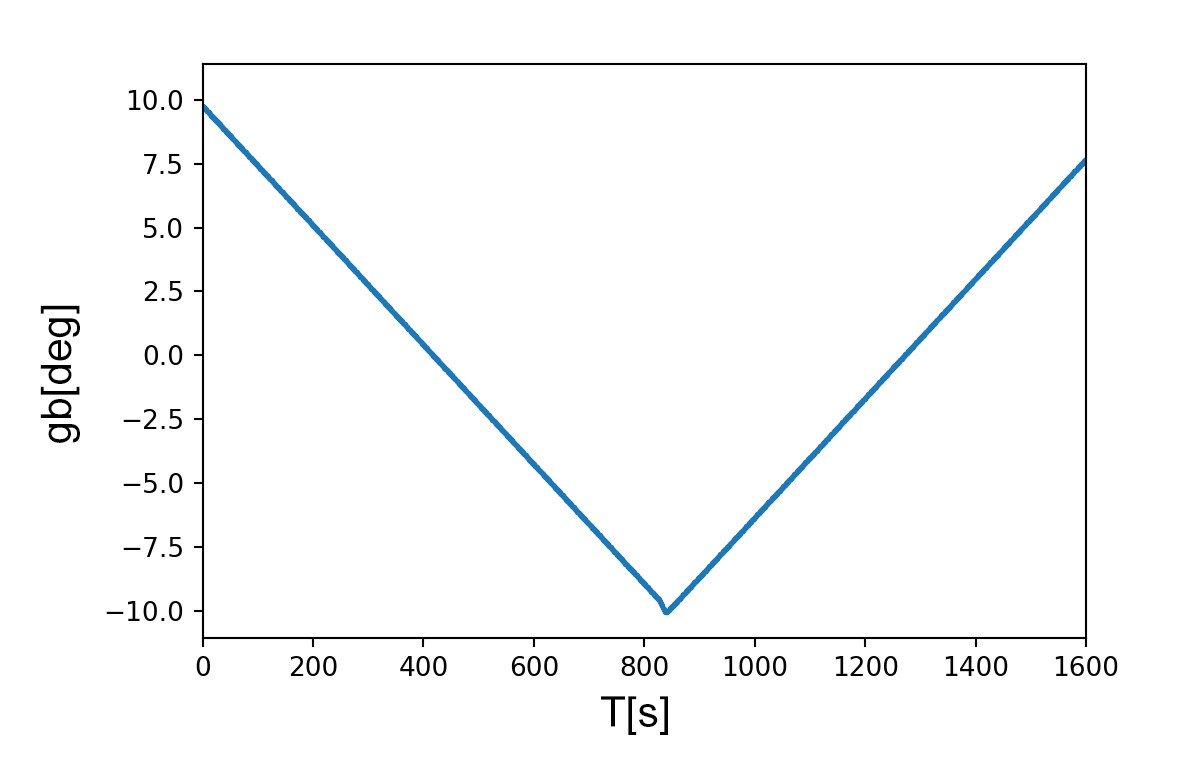
\includegraphics[width=0.58\textwidth]{figures/gs/01634_0001-gb-new}
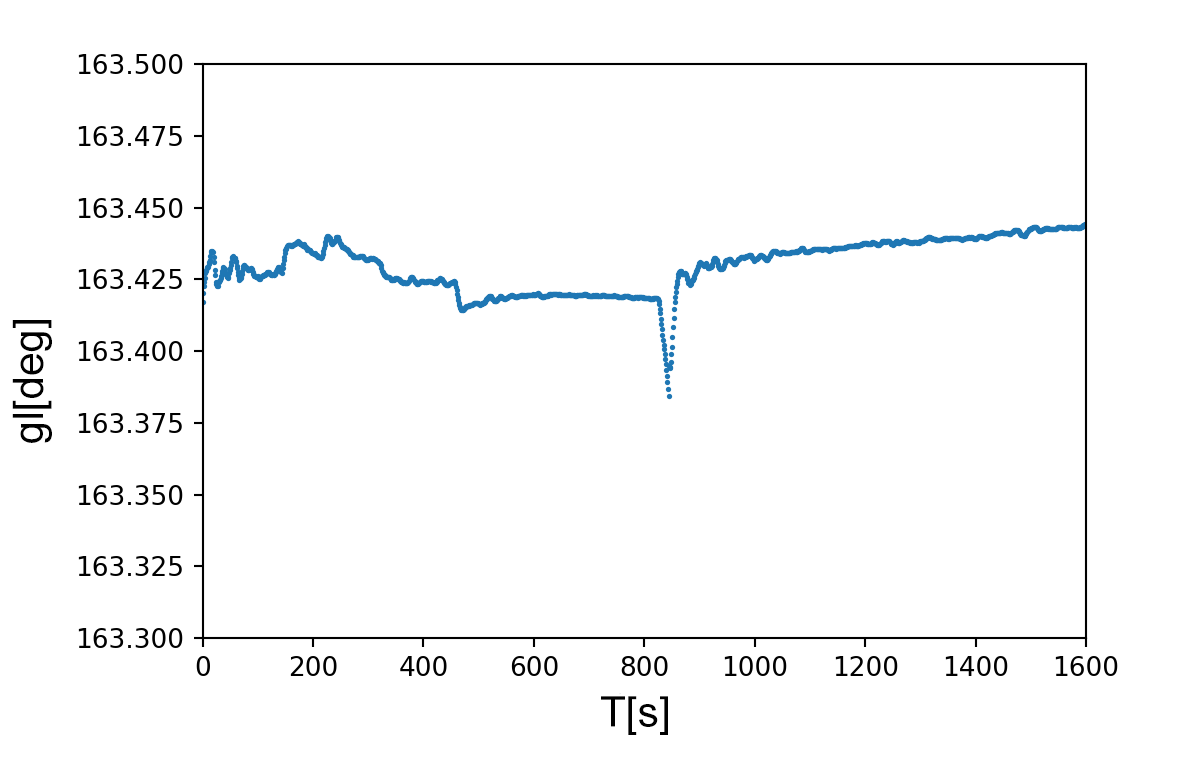
\includegraphics[width=0.58\textwidth]{figures/gs/01634_0001-gl-new}
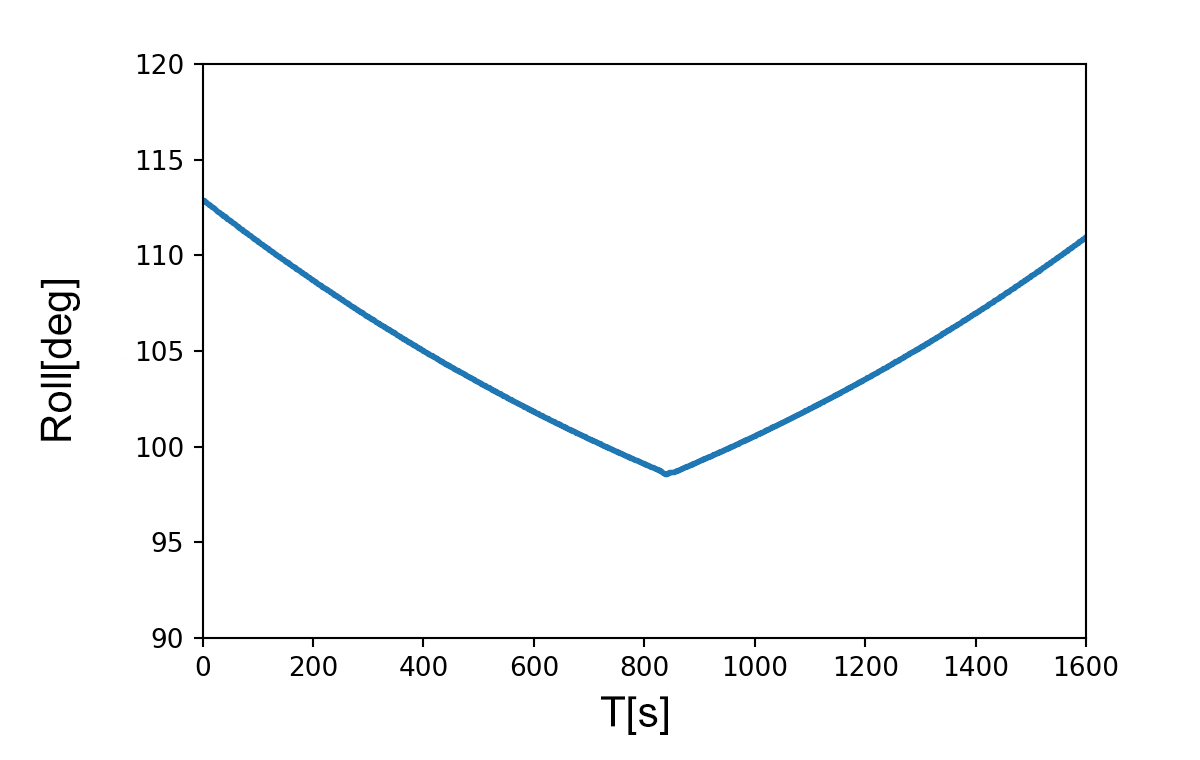
\includegraphics[width=0.58\textwidth]{figures/gs/01634_0001-roll-new}
\end{center}
\caption[The \galex\ telescope pointing and roll change during one scan]{%
  \label{telescope}
  An example shows how the \galex\ telescope pointing and roll change during one scan.
  The telescope traversed the Galactic plane twice during one scan and maintain the pointing in $gl$ nearly unchanged.
  There are 450 scans similar to this observed during the \scanmode. 
  \emph{Top:}  Pointting in $gb$ as a function of time;
  \emph{Middle:} Pointting in $gl$ as a function of time;
  \emph{Bottom:} Roll in Equatorial coordinates changes as a function of time.
}
\end{figure}

\begin{figure}[p]
\begin{center}
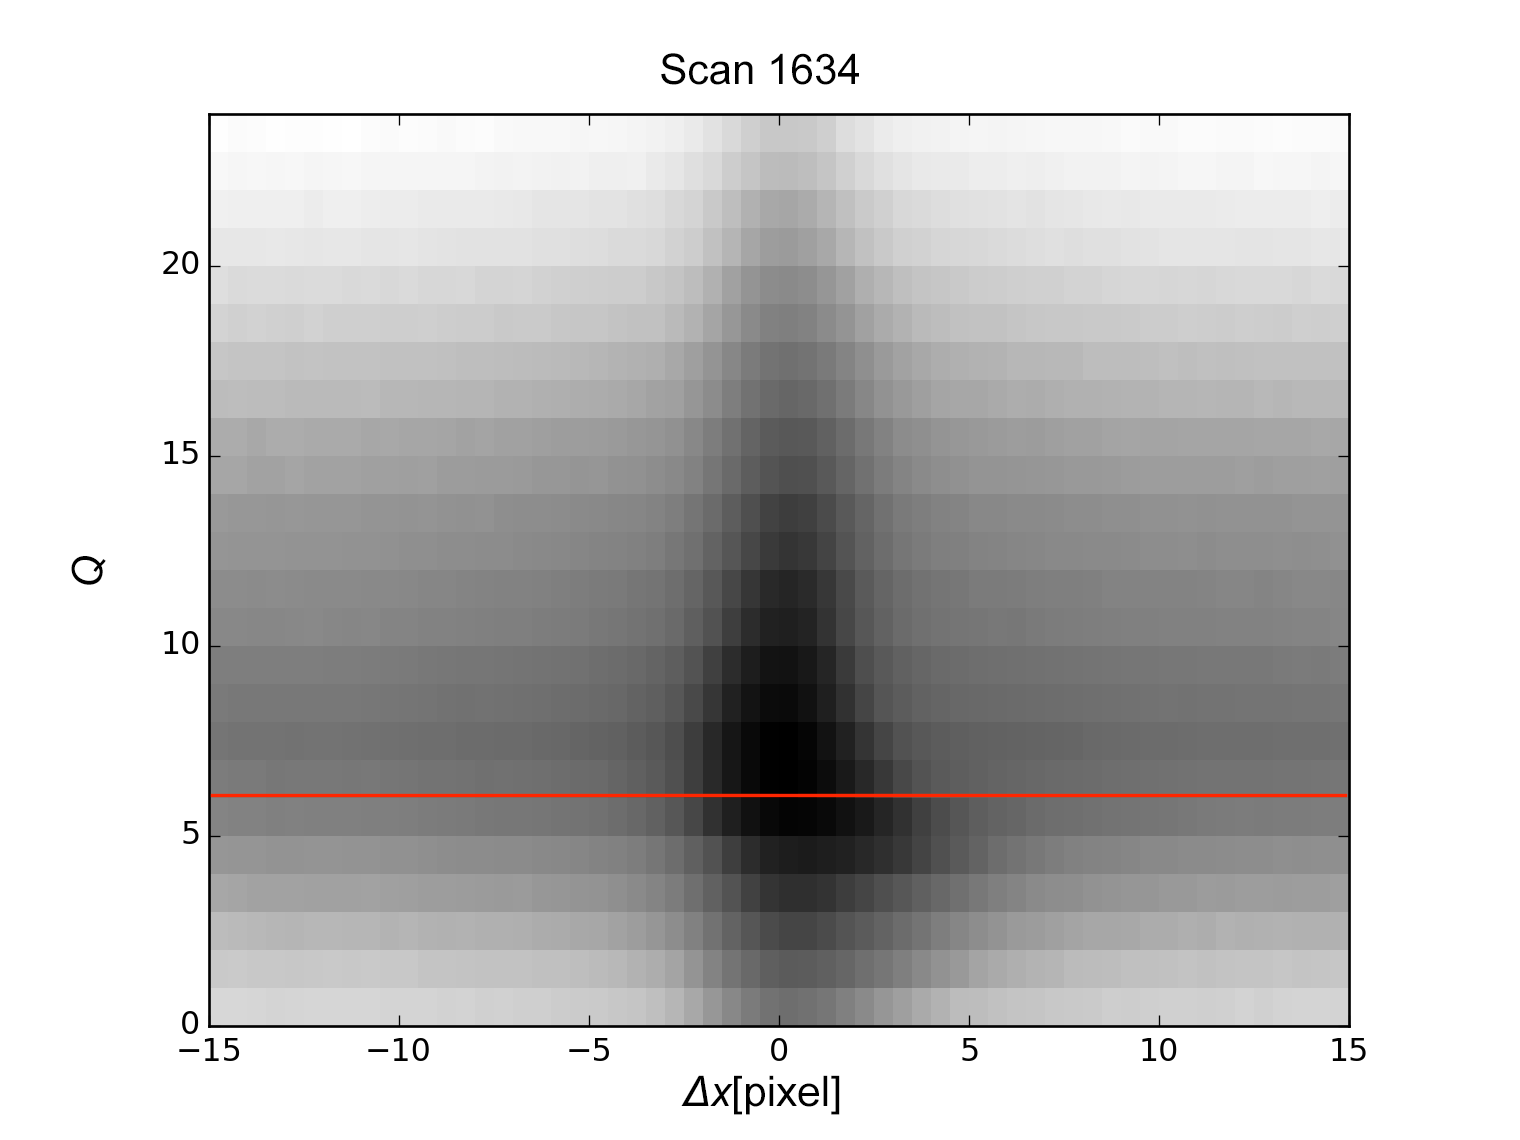
\includegraphics[width=0.49\textwidth]{figures/q-x_tot-new}
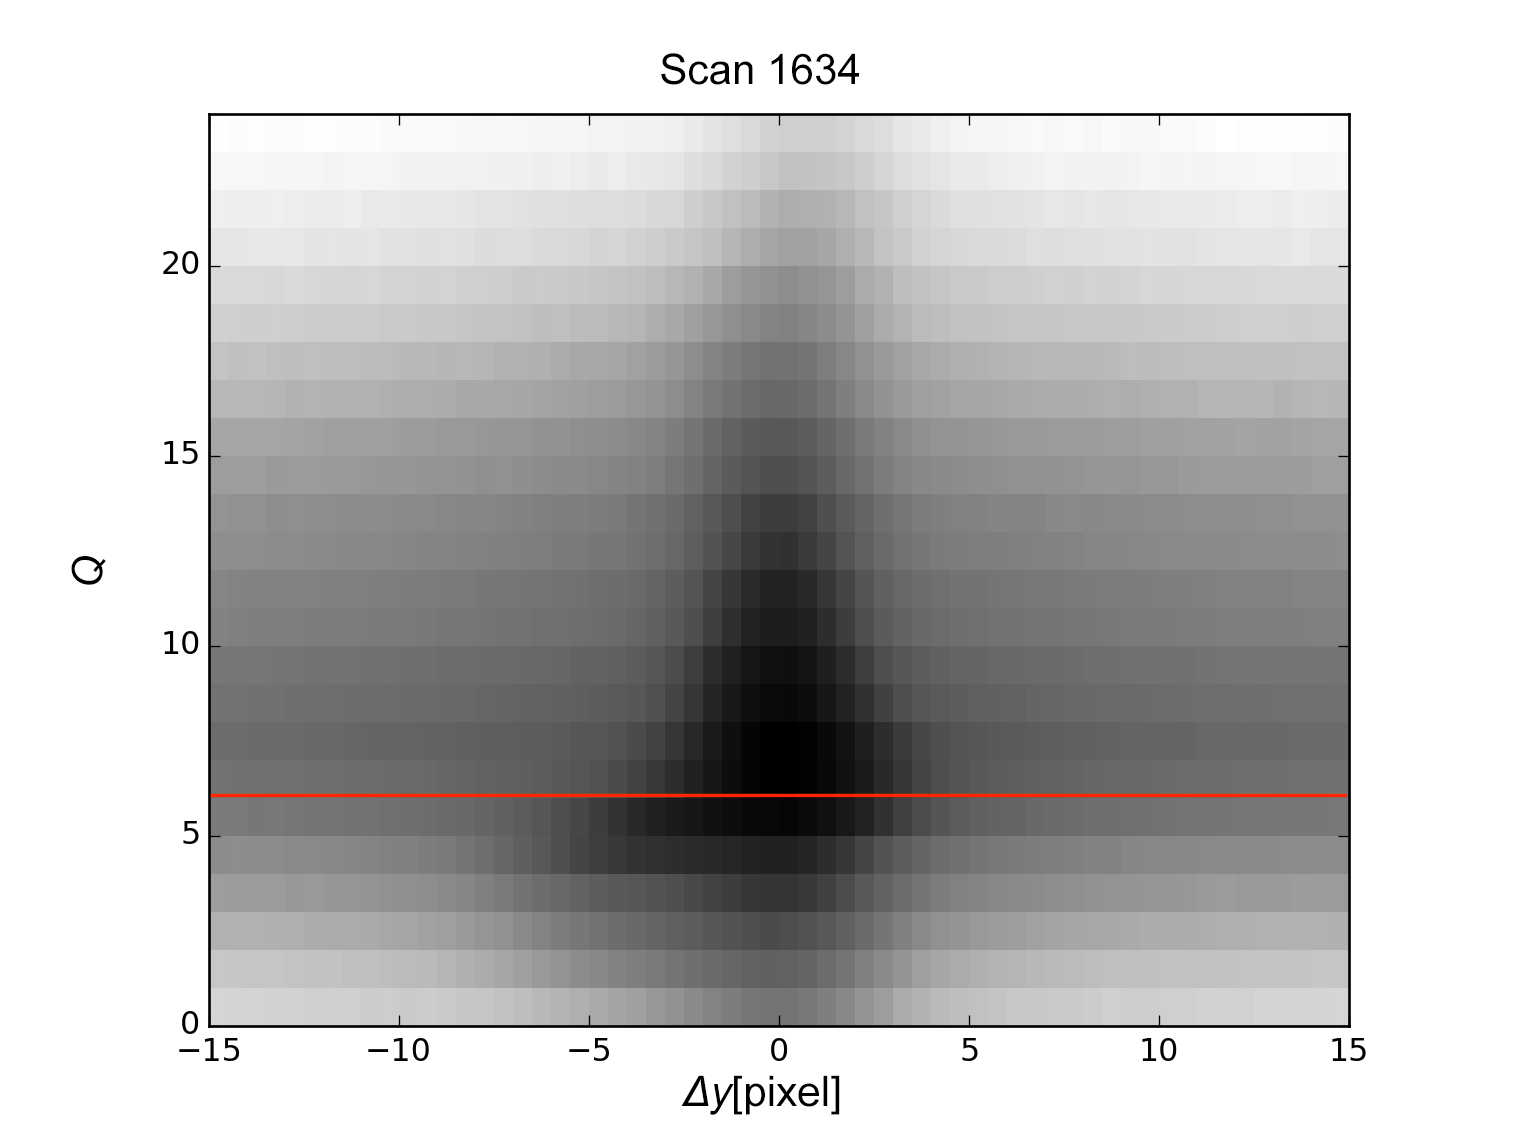
\includegraphics[width=0.49\textwidth]{figures/q-y_tot-new}
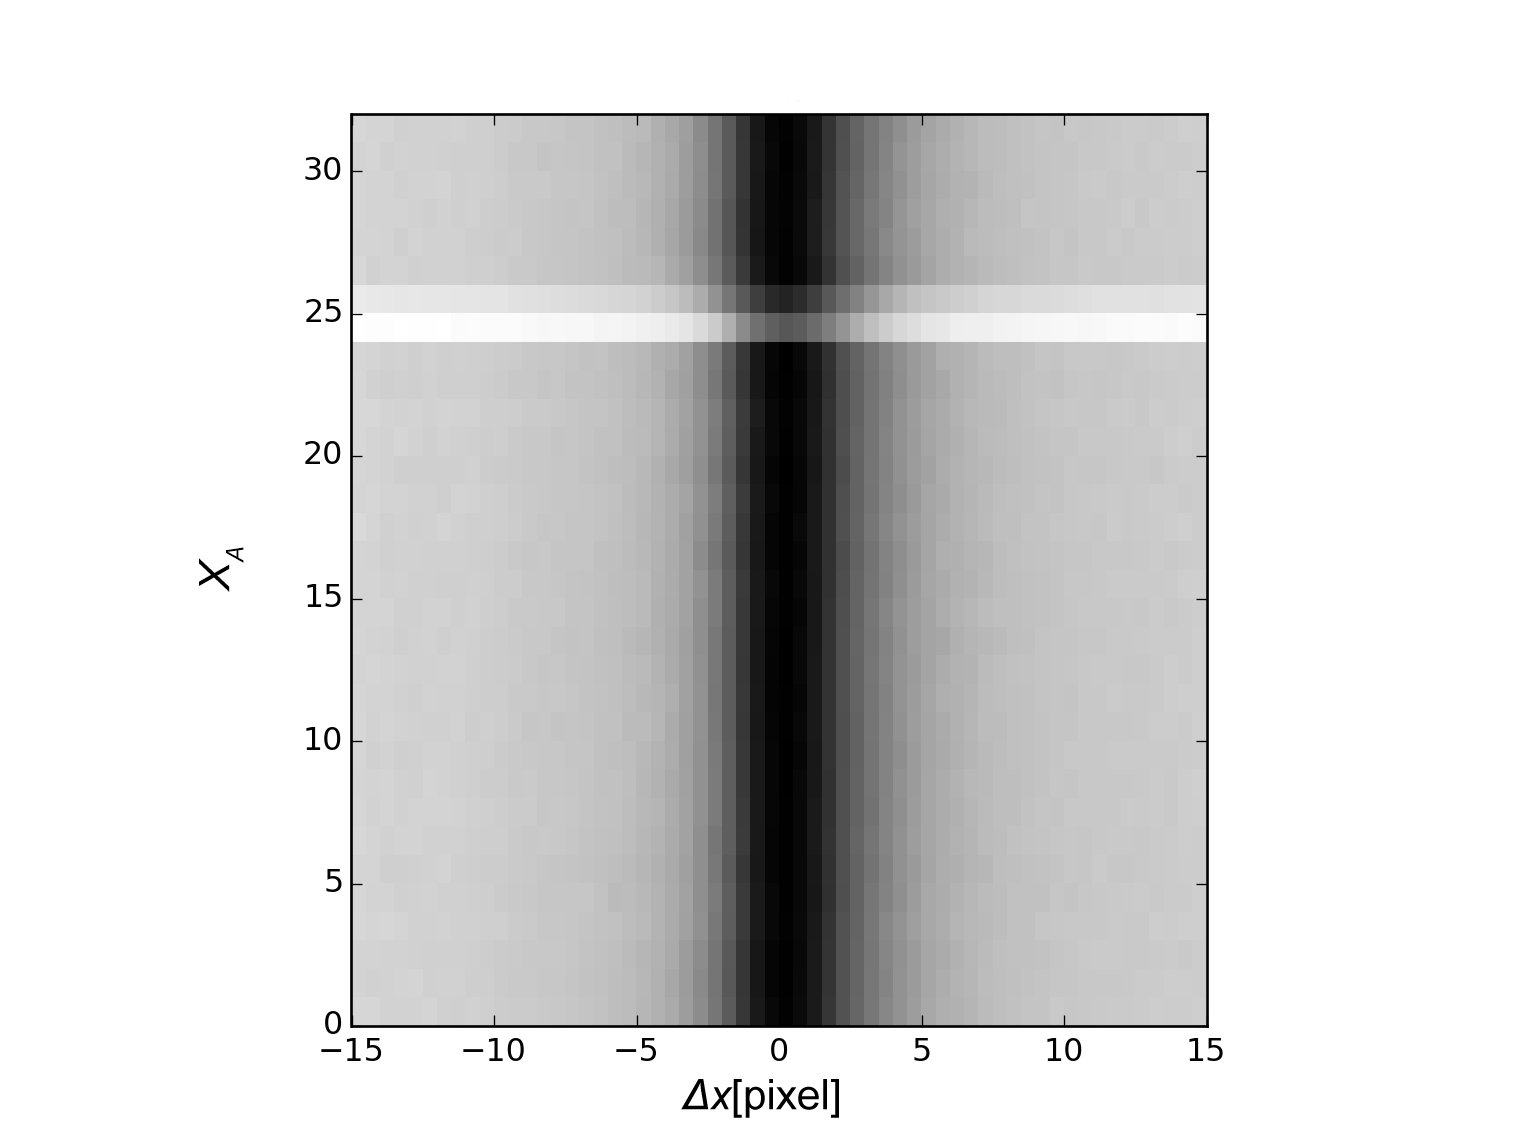
\includegraphics[width=0.49\textwidth]{figures/xa-x_tot-new}
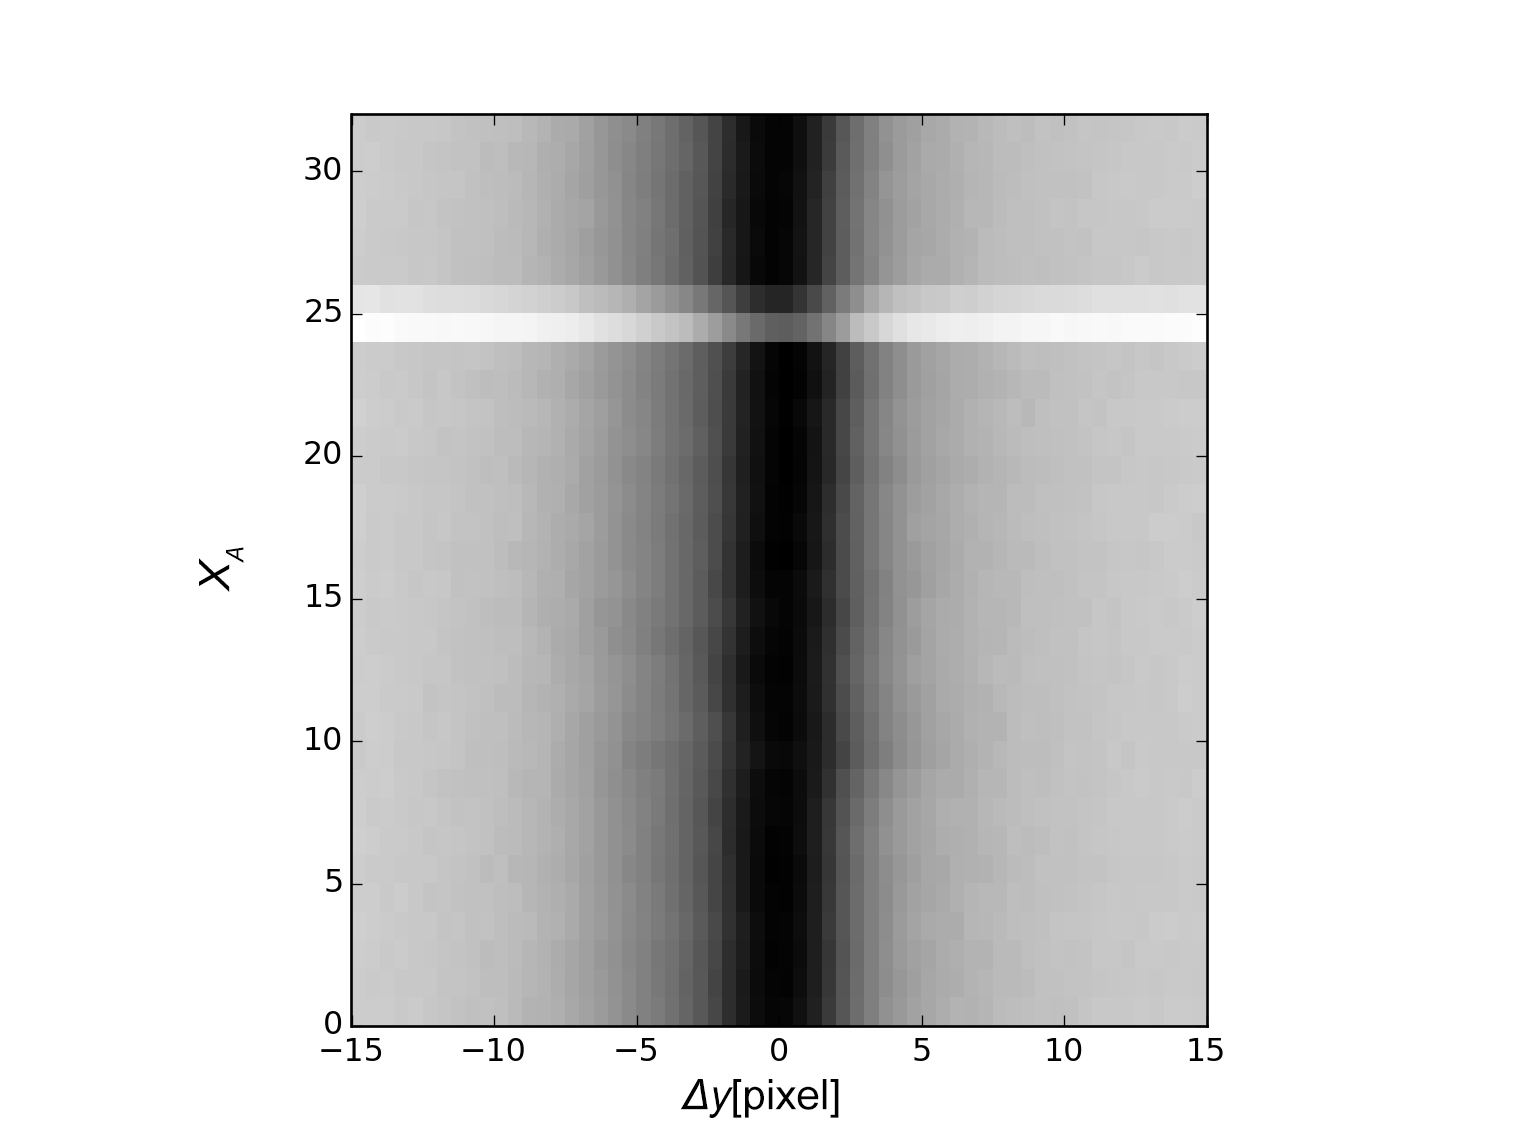
\includegraphics[width=0.49\textwidth]{figures/xa-y_tot-new}
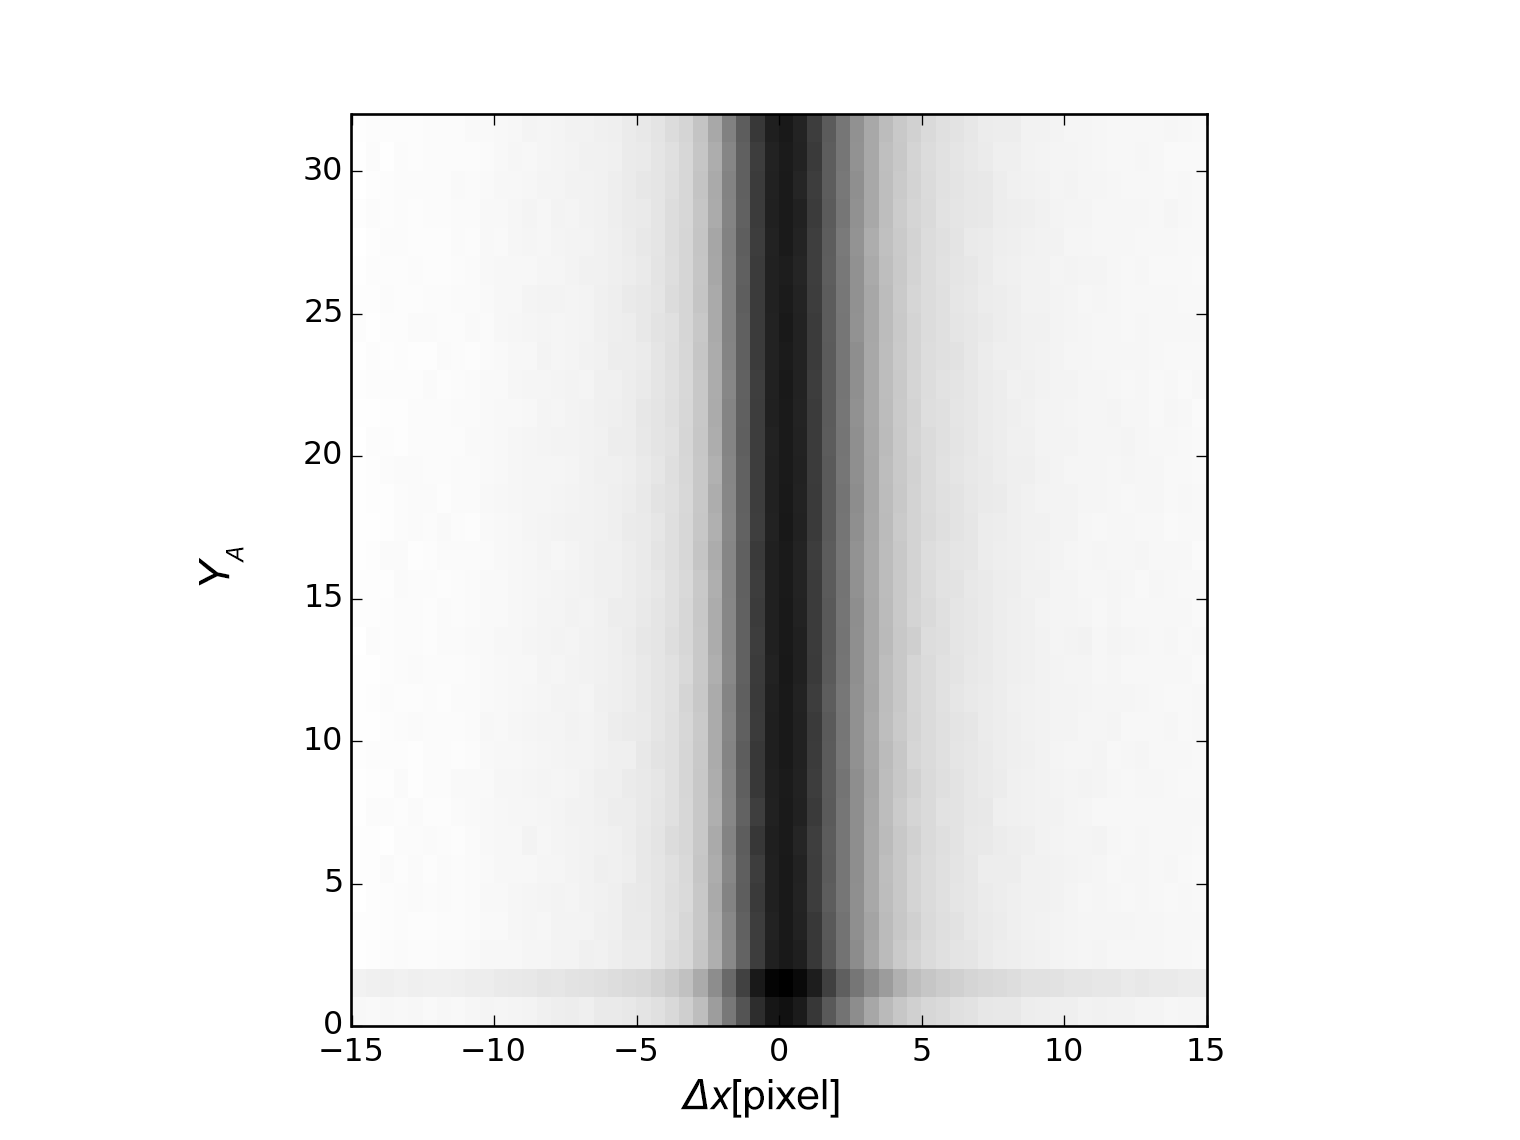
\includegraphics[width=0.49\textwidth]{figures/ya-x_tot-new}
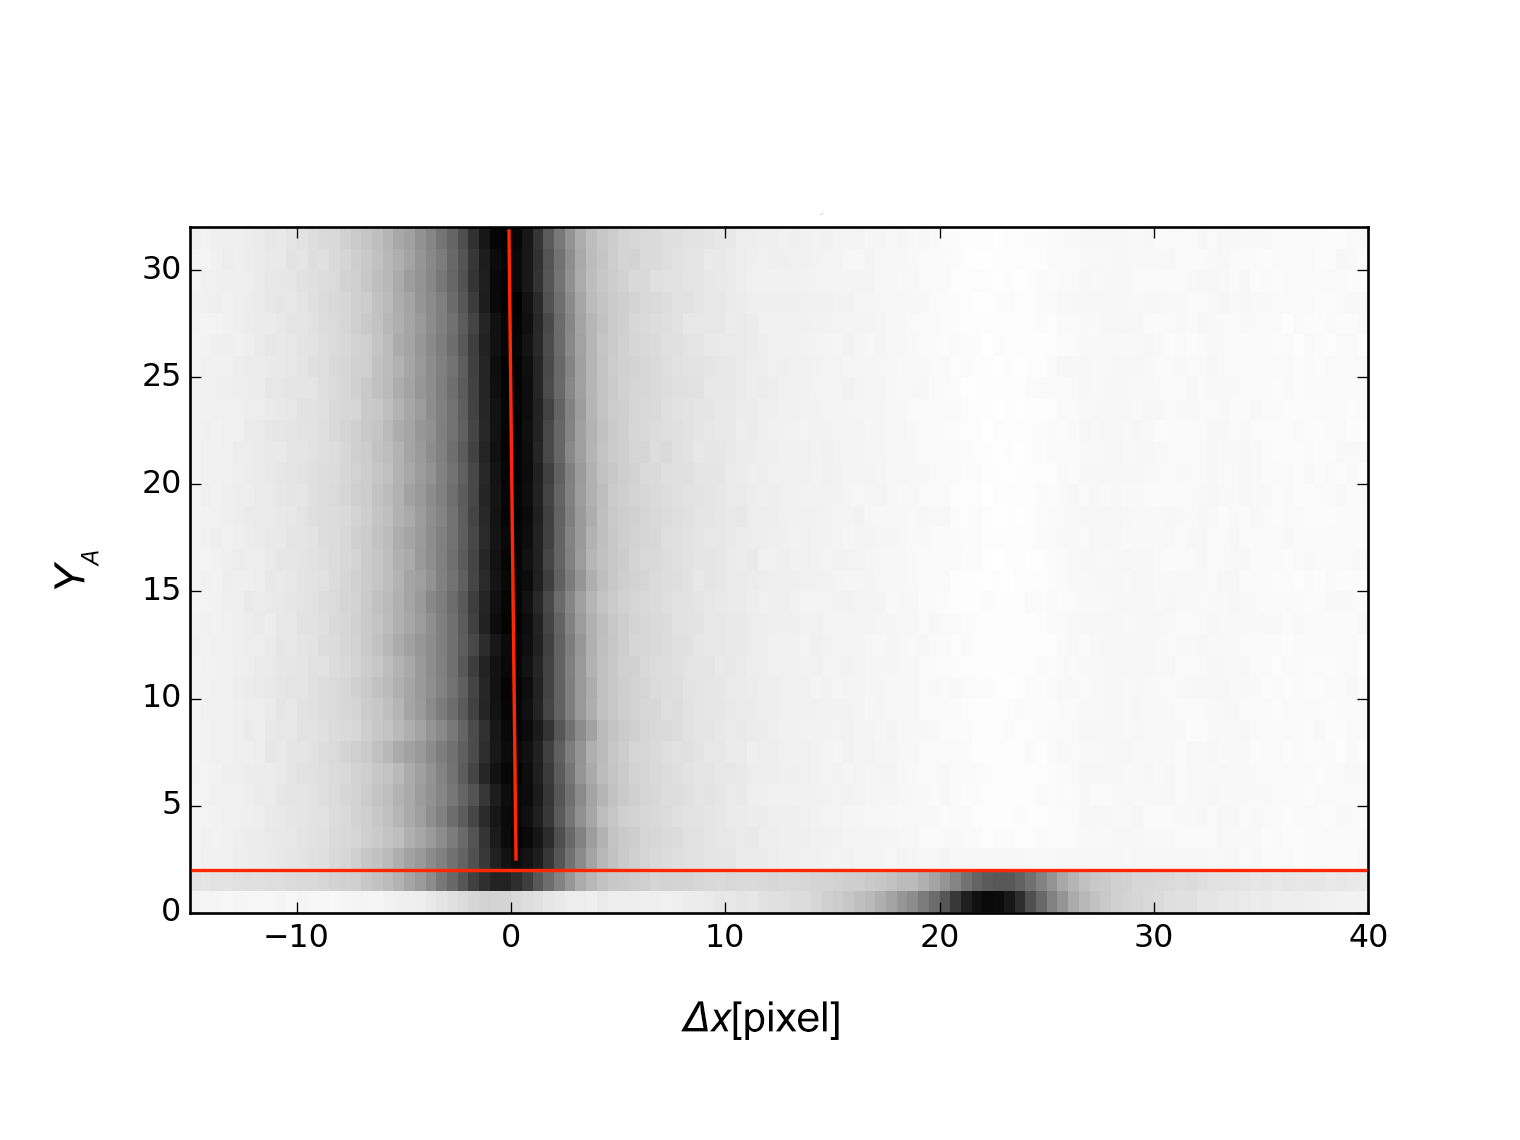
\includegraphics[width=0.49\textwidth]{figures/ya-y_tot-new}
\end{center}
\caption[Overall offsets of photons as function of pulse height $Q$,  wiggle (the phase of the TAC)  $X_A$,  stim spread slope $Y_A$]{%
  \label{meta}
  Overall offsets of photons as function of pulse height $Q$,  wiggle (the phase of the TAC)  $X_A$,  stim spread slope $Y_A$.
  Photons below the horizontal red lines are removed from the photon list.
  }
\end{figure}

\section{Pointing calibration}
\label{pc}
As mentioned in Section \ref{data}, the \galex\ photons are tagged with time, position on the detector and other housekeeping information($Q$, $X_A$ and $Y_A$).
To use these photons such as constructing sky-maps, the pointing of the spacecraft is required as an input of the 
\project{gPhoton} to project the photons onto the sky.
Due to the control and knowledge errors of \galex, the pointing recorded on the flight is not perfect, especially in the \scanmode, in which the spacecraft traversed the galactic plane rapidly. 
In this paper, as was done in the main \galex\ pipeline, we are going to use the photons together with the stars catalog to calibrate the pointing of the spacecraft and refine the attitude solution.
The top plot in Fig.~\ref{slice} shows an one-second snapshot of the photons on the sky.
The stars from Tycho 2 catalog \citep{tycho2} in the same region are also plotted. 
It is obvious that there is an significant overall offset between the stars (cross-hair) and photons (points),  which is due to the imperfection of the pointing.
To characterize the offsets of the pointing of the spacecraft, the cross-correlation of photons and star catalog are calculated.
The cross-correlation $\xi(\vec{r})$ is defined as the count of photon-star pairs as a function of displacement $\vec{r}$.
As shown in the bottom plot of Fig.~\ref{slice}, the offsets of the pointing are determined by the centroid of the cross-correlation function.
Because the position errors in the star catalog are small, much less than 1", the shape of the correlation function is dominated by the \galex\ point spread function (PSF).
There is also a secondary peak in the cross-correlation function due to the photons with $Y_A<2$, which has been explained in Section \ref{data} and can be removed by cutting the photon list.
After photons are binned in one-second slots, the offsets of pointing can be measured as a function of time as shown in Fig.~\ref{pointing}.
By utilizing the cross-correlation between photons and stars, we can figure out pointing using stars, but without ever actually running any kind of star detector in the raw data. 
The point is that we avoid any choices about how stars are detected.

\begin{figure}[p]
\begin{center}
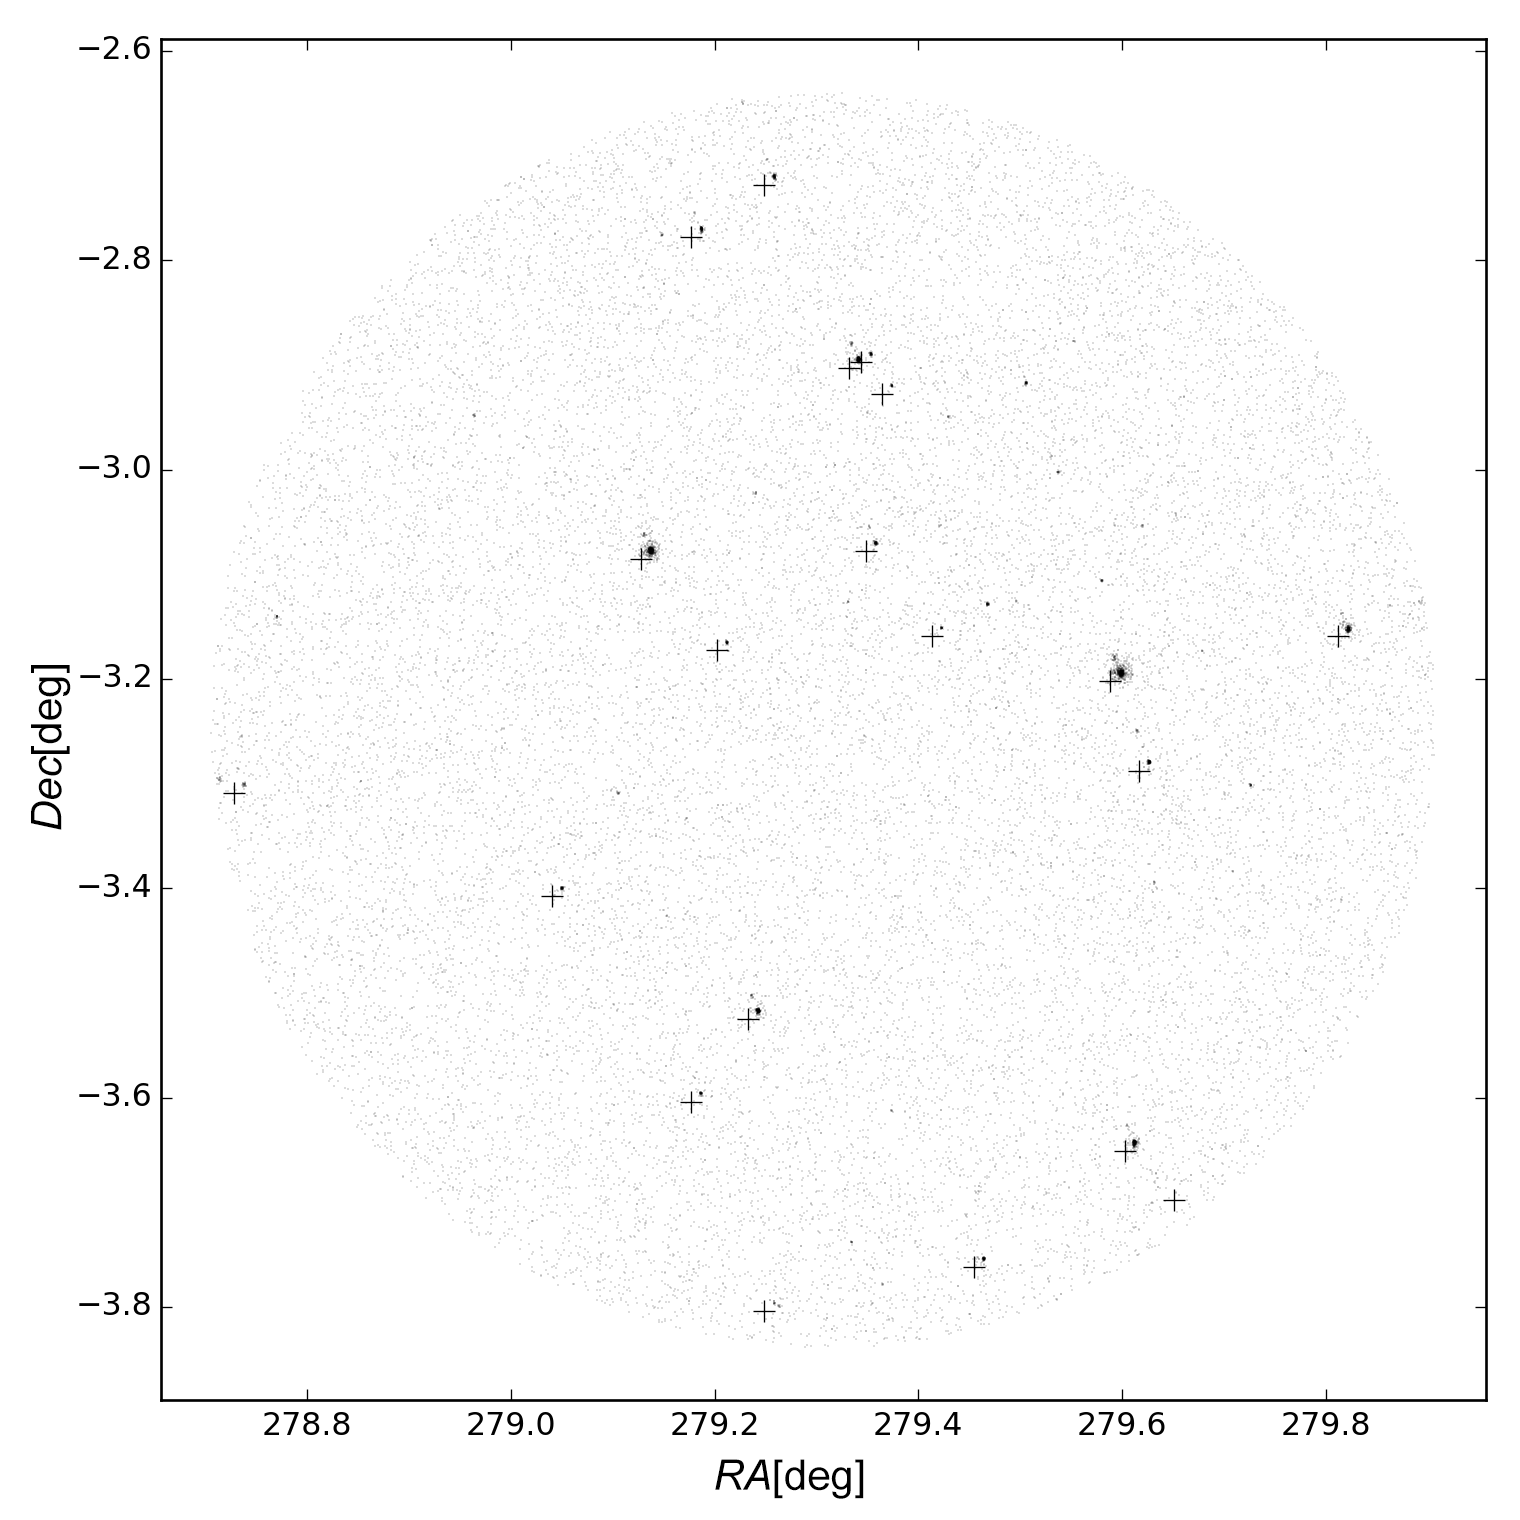
\includegraphics[width=0.535\textwidth]{figures/gs/photons600-new}
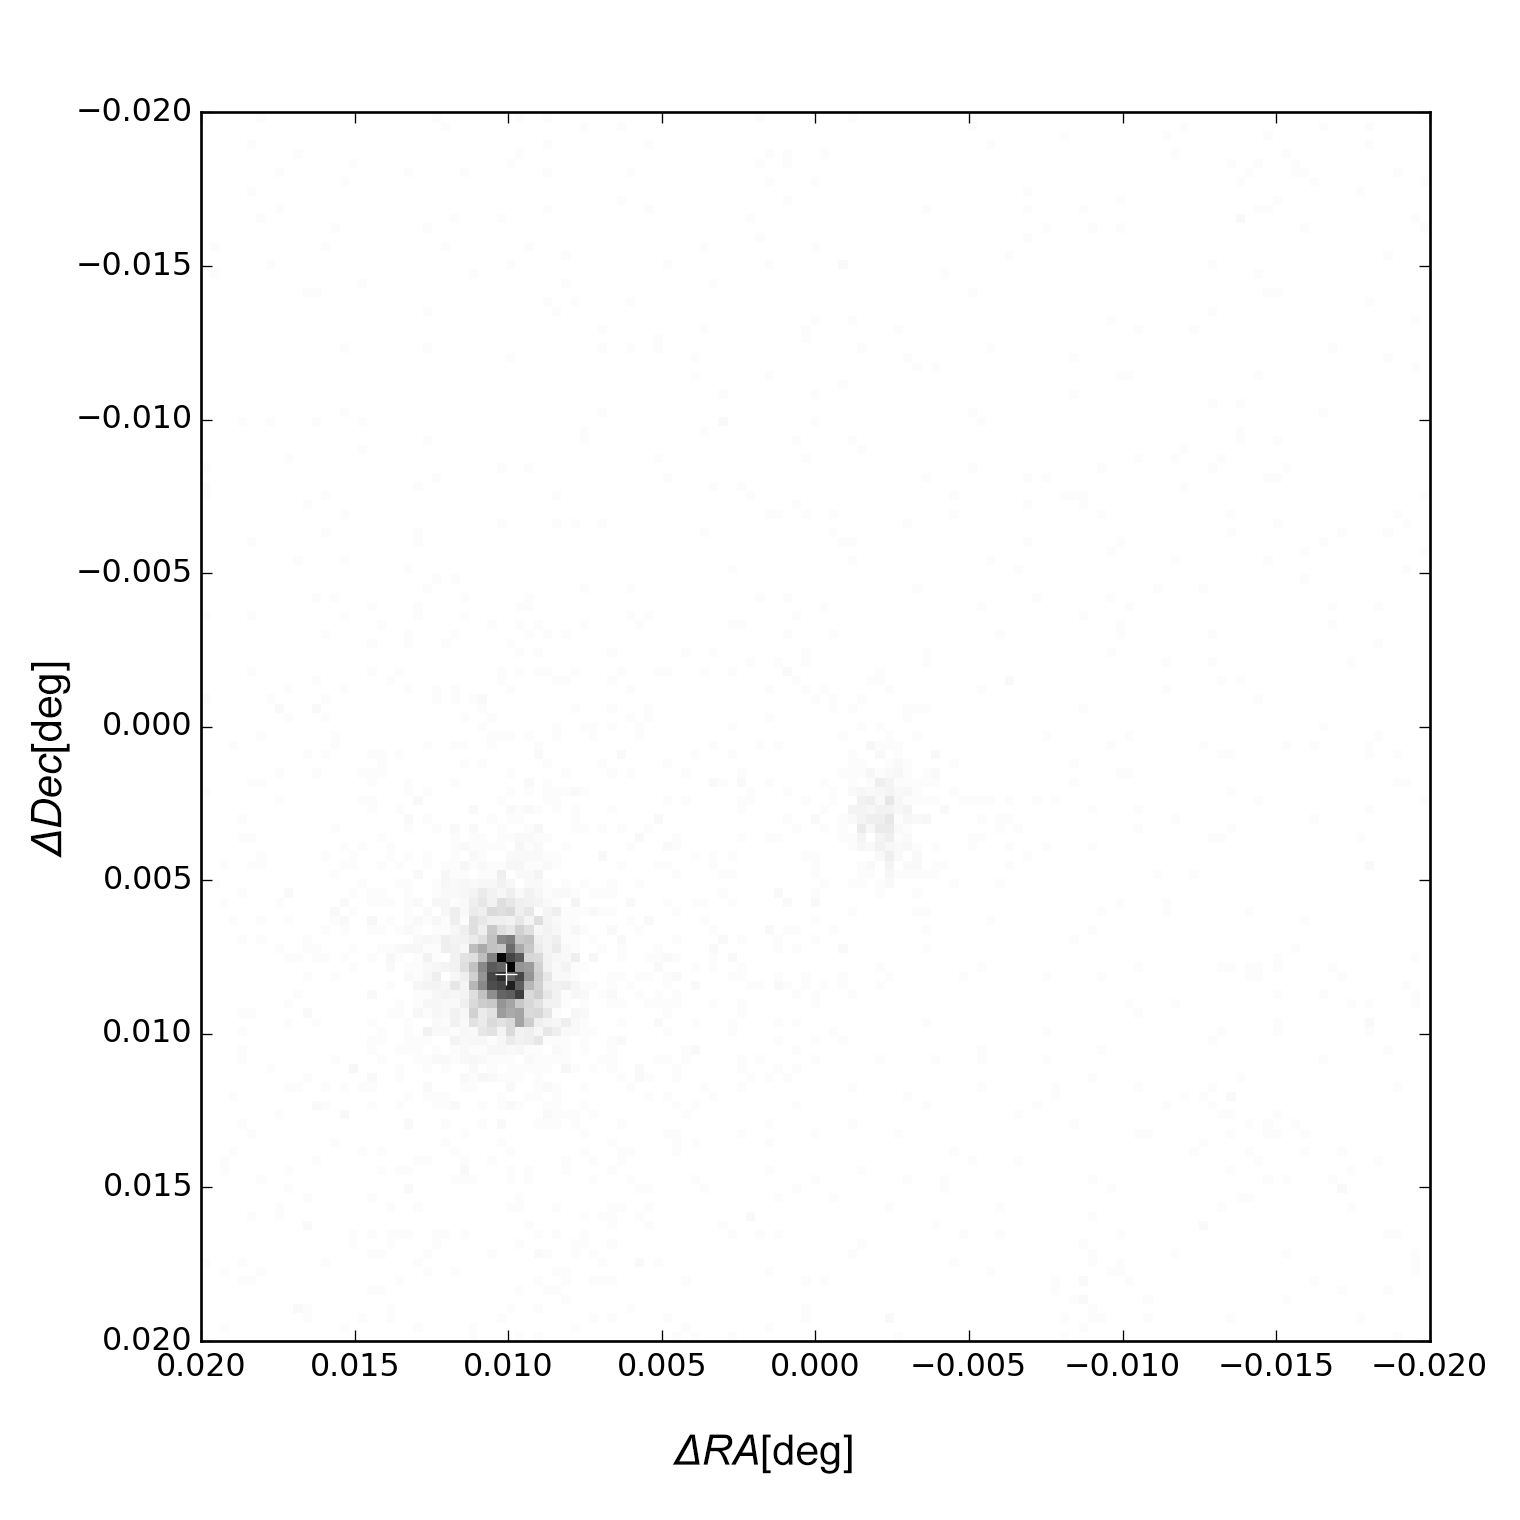
\includegraphics[width=0.58\textwidth]{figures/gs/co600-new}
\end{center}
\caption[Cross-correlation of photons and star catalog]{%
  \label{slice}
  Cross-correlation of photons and star catalog.
  \emph{Top:}  An one-second snapshot of the photons on the sky. The points are the location of the photons. The crosses indicate the location of the stars from the input catalog. It is obvious that there is a small offset between photons and the stars.
  \emph{Bottom:} The cross-correlation of photons and stars. 
  Each black points in the plot shows the offset between a pair of photon and star.
  The distribution of balck points corresponds to the "reconstructed" PSF in this iteration. 
  The white cross indicates the centroid of the the black points, which is the overall offsets between photons and stars---the offset of the pointing.
  }
\end{figure}

\begin{figure}[p]
\begin{center}
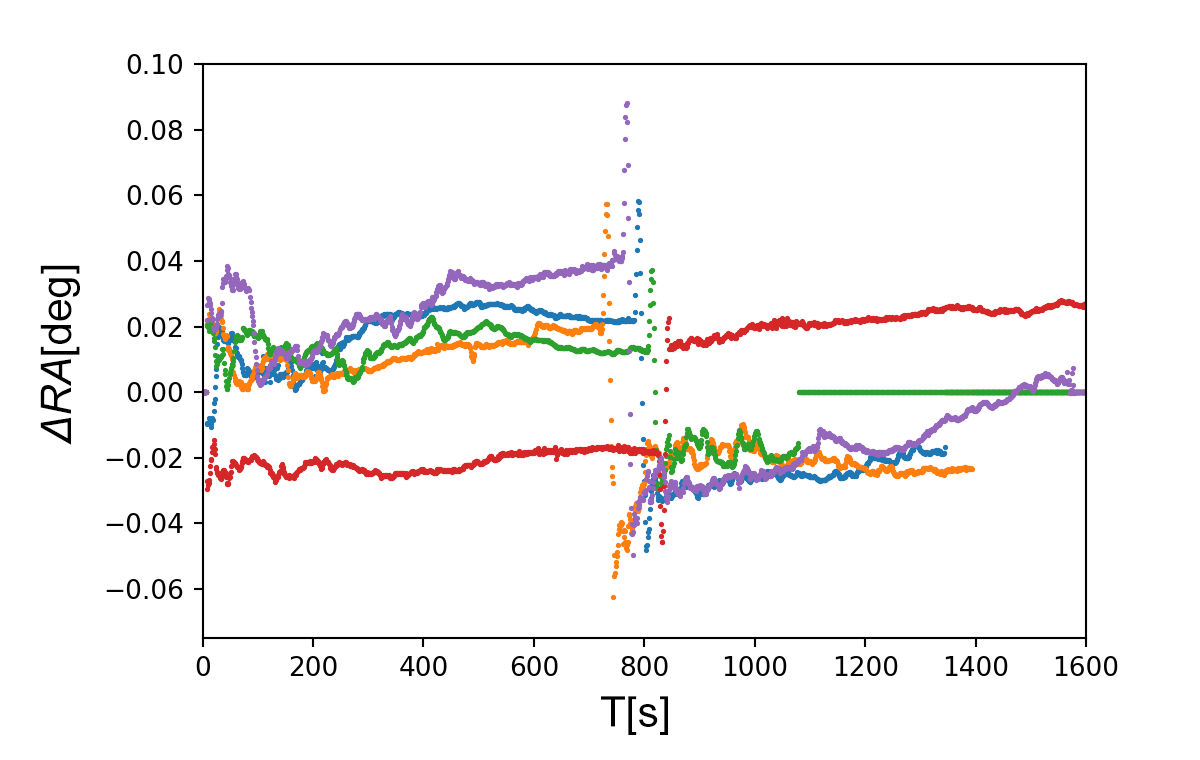
\includegraphics[width=0.6\textwidth]{figures/gs/all-ra-new}
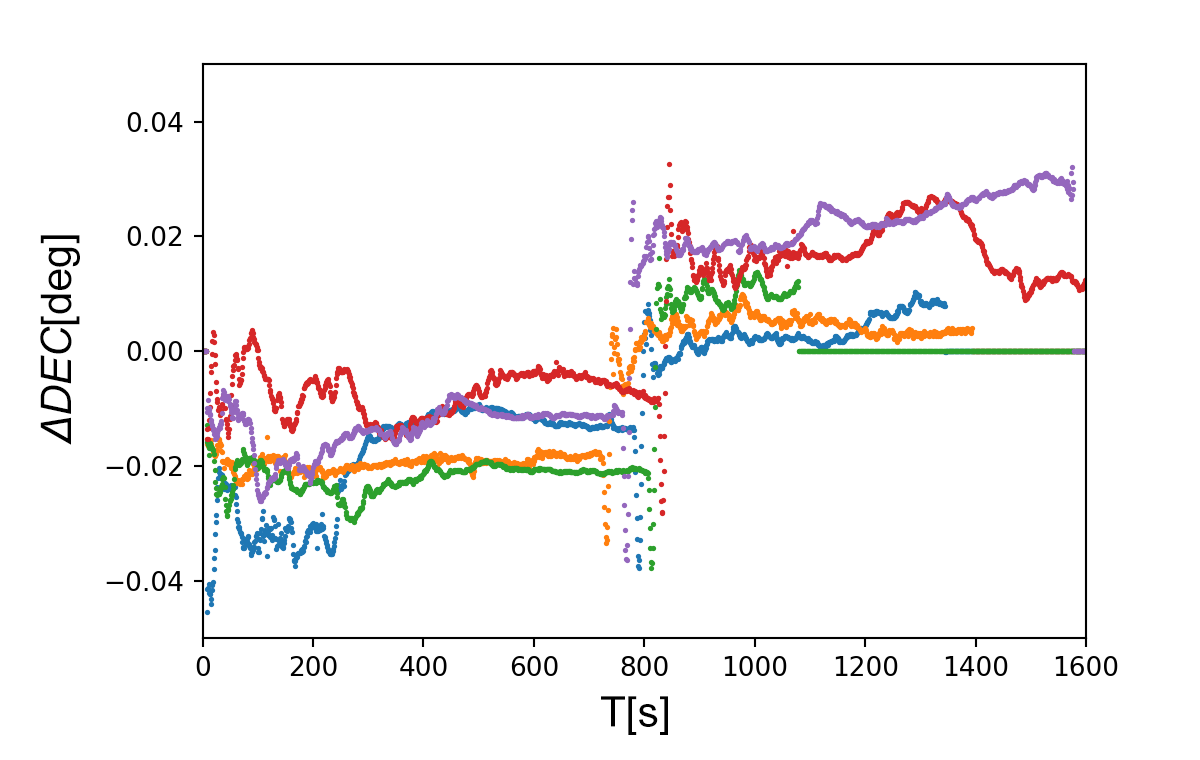
\includegraphics[width=0.6\textwidth]{figures/gs/all-dec-new}
\end{center}
\caption[Spacecraft pointing offsets as a function of time]{%
  \label{pointing}
  Pointing offsets as a function of time.
  \emph{Top:}  Pointing offsets in RA as a function of time.
  \emph{Bottom:} Pointing offsets in Dec as a function of time.
  The dramtical changes around 800s is due to the reversal of the spacecraft scan rate when the boresight position reaches $gb=-10 deg$, designed to occur at a time near the center of the orbital eclipse.
  }
\end{figure}

\section{Distortion map}
\label{dm}
Except for the overall offset due to the pointing, there is also local error in photon position caused by the detector. 
According to \cite{galex_cal}, the photon position on \galex\ detector was measured by the arrival time difference of pulses from either side of the delay line anode, while the time difference consists of an integer number of coarse clock step and a fine position (phase of the coarse clock).
The fine position is measured as voltage value by time-to-amplitude converter (TAC).
Due to the electronic nonlinearity of TAC, each photon event can have a small local error in position and this effect is recorded as a function of $X_A$ value in the photon list.
In addition to the nonlinearity of TAC, the variations in gain also affect the position of the photon events.
The gain effect is recorded as pulse height $Q$ in the photon list.
To calibrate these local effects on the detector, in this paper, a distortion map is constructed by a similar method in Section \ref{pc}.  
The detector is divided into 50 by 50 grid pixels. 
Within each grid pixel, the stars are projected onto the detector with the pointing measured in section \ref{pc}.
Then the photons and stars are cross-correlated and the centroid of the correlation function is measured as the distortion in that pixel location.
In Fig.~\ref{distortion_xa}, the photons are binned into three subset by the $X_A$ value and the distortion-map of each subset photons is constructed.
The amplitude of the distortion is about 0.03 grid pixels, which is approximately around $\sim 2"$ on the sky.
There is significant difference between distortion-map constructed with different subset of photons.
The difference shows a periodic pattern over the detector, a significant component of which appears to be correlated with the phases of the coarse clock ($X_A$)
Similarly Fig.~\ref{distortion_q} shows the distortion-map constructed with photons of different $Q$ values.

\begin{figure}[p]
\begin{center}
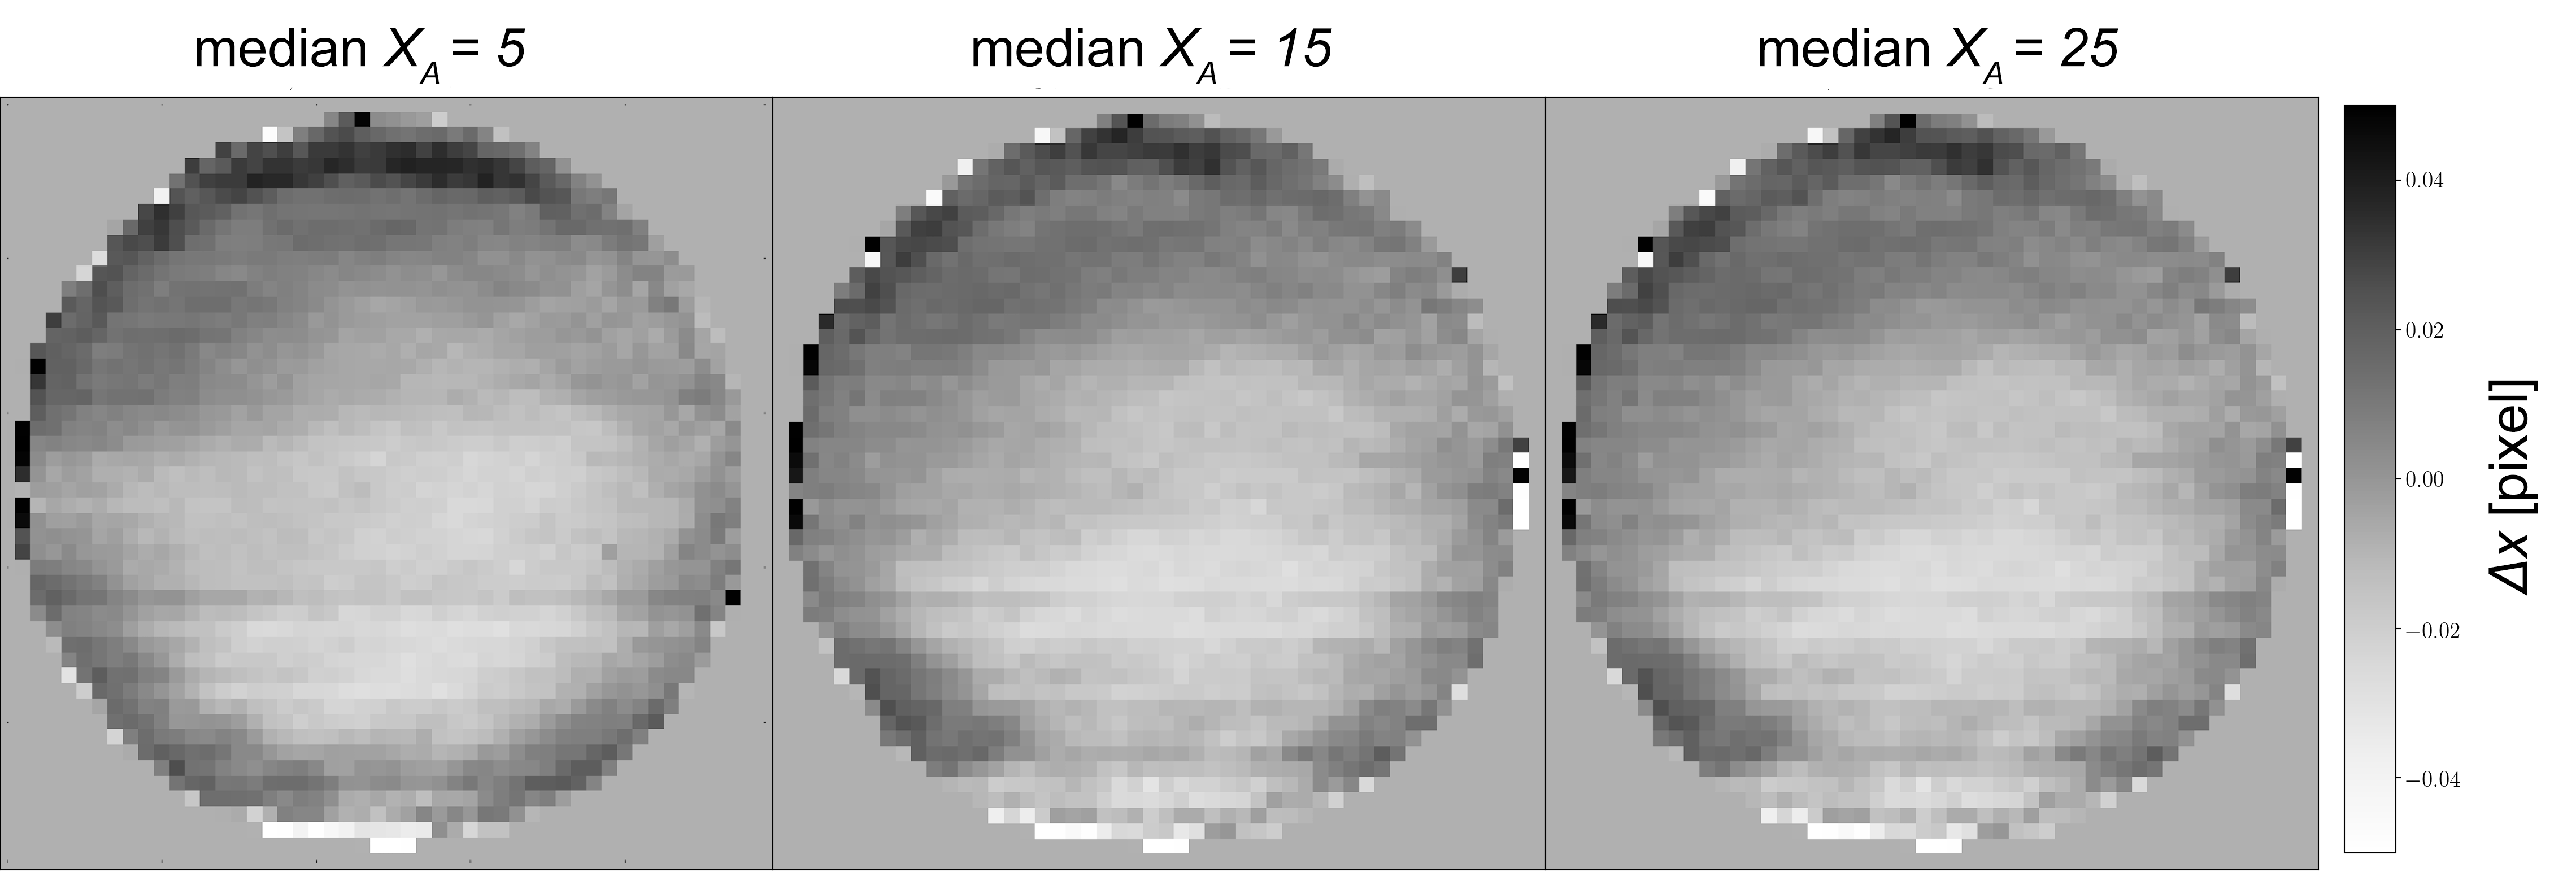
\includegraphics[width=0.95\textwidth]{figures/gs/xa-x-new}
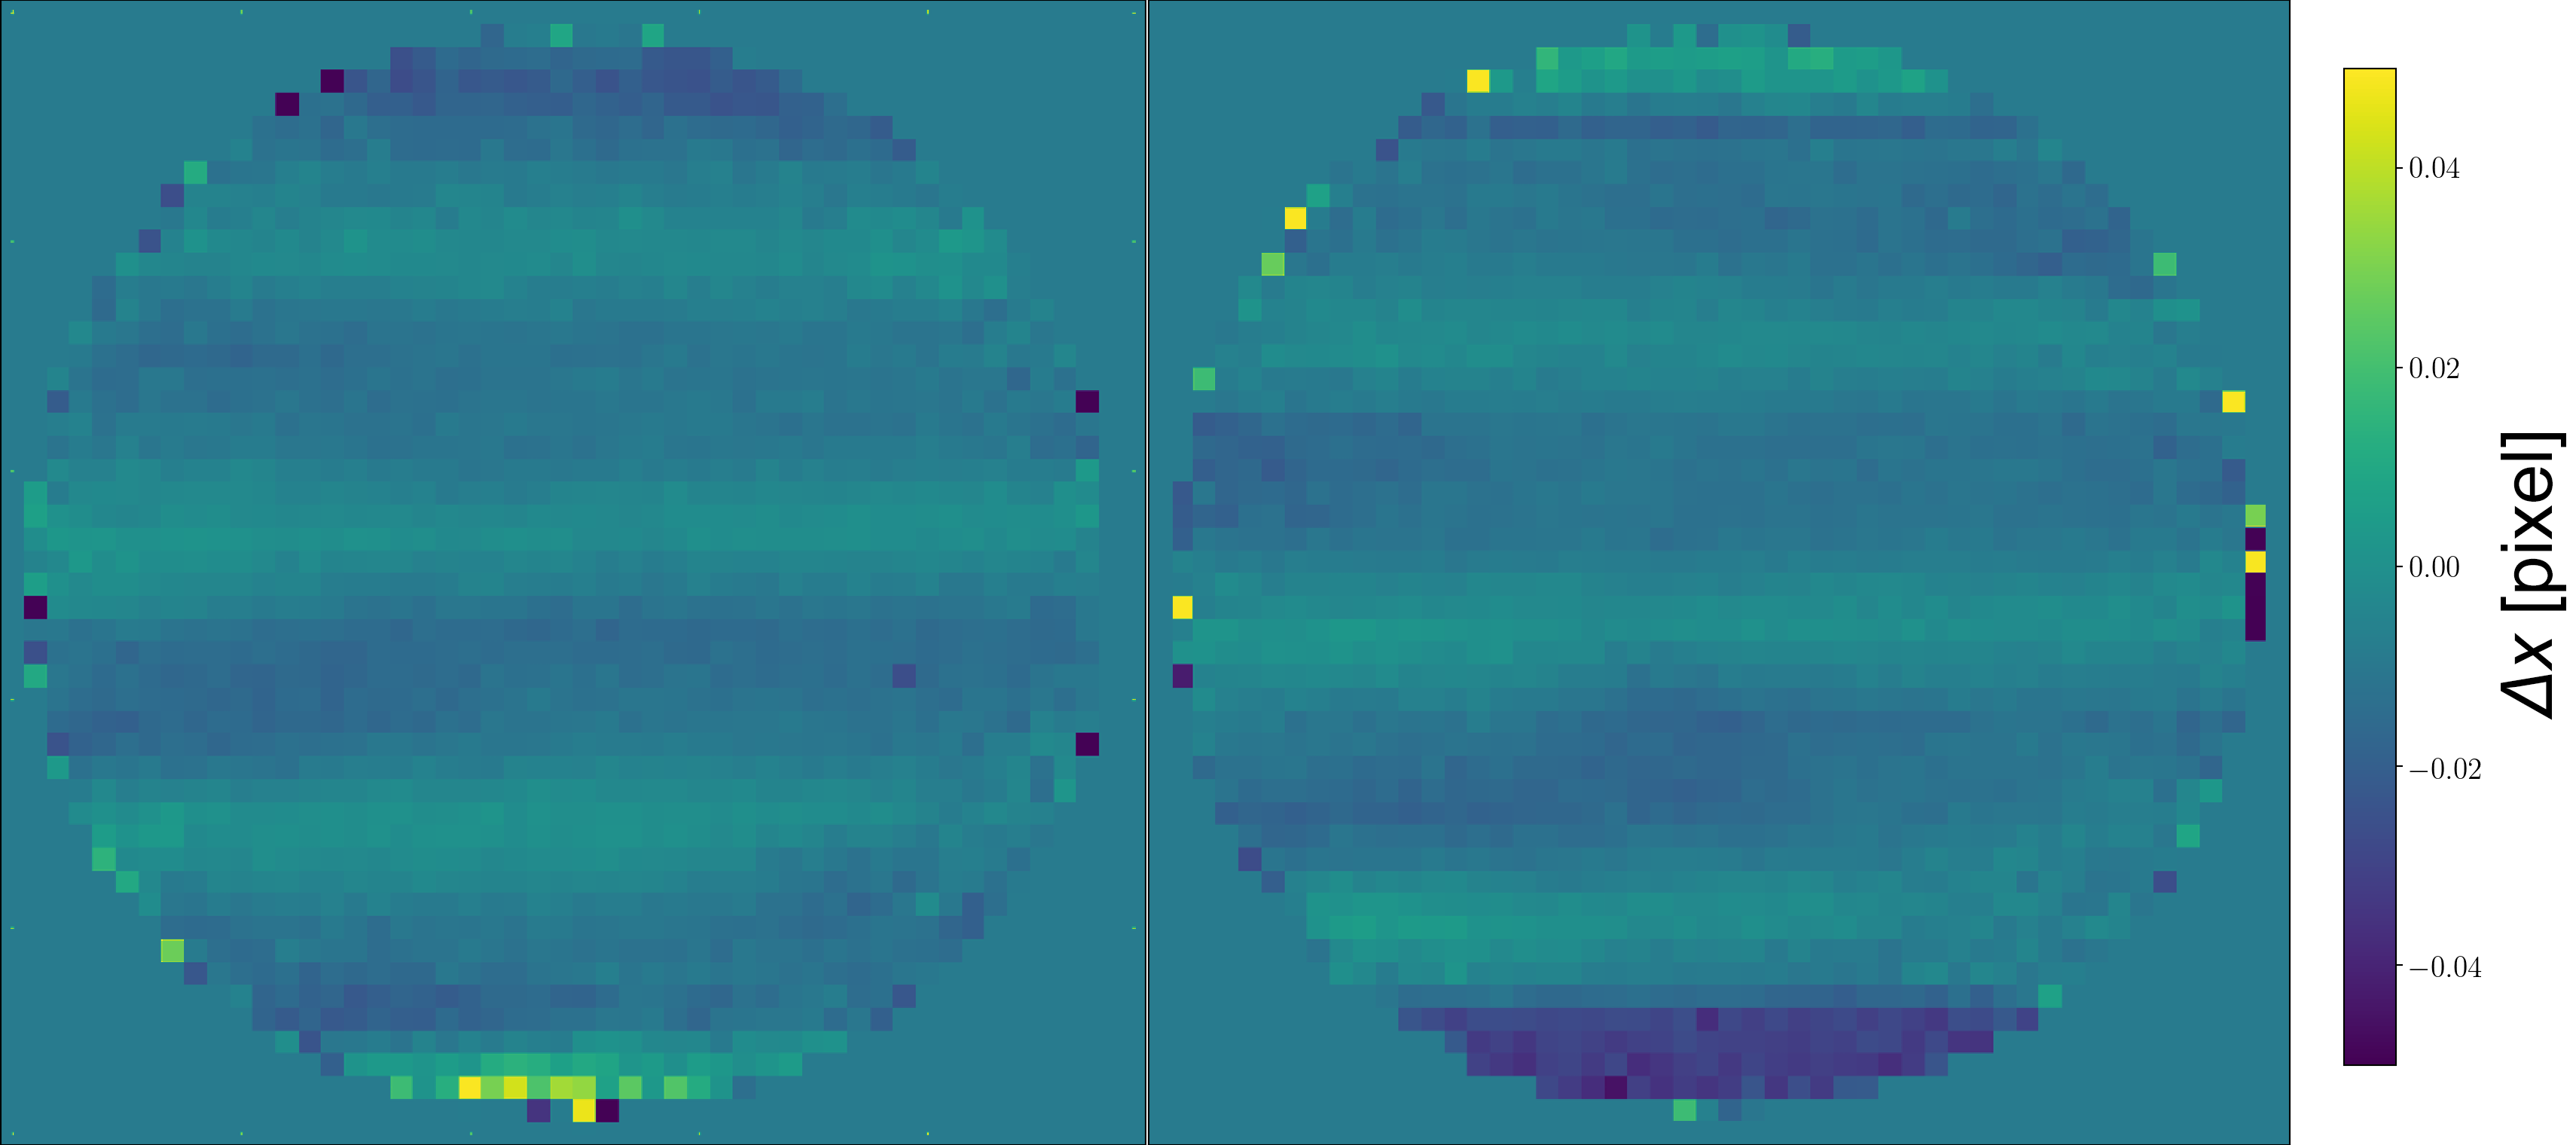
\includegraphics[width=0.6\textwidth]{figures/gs/dif-xa-x-new}
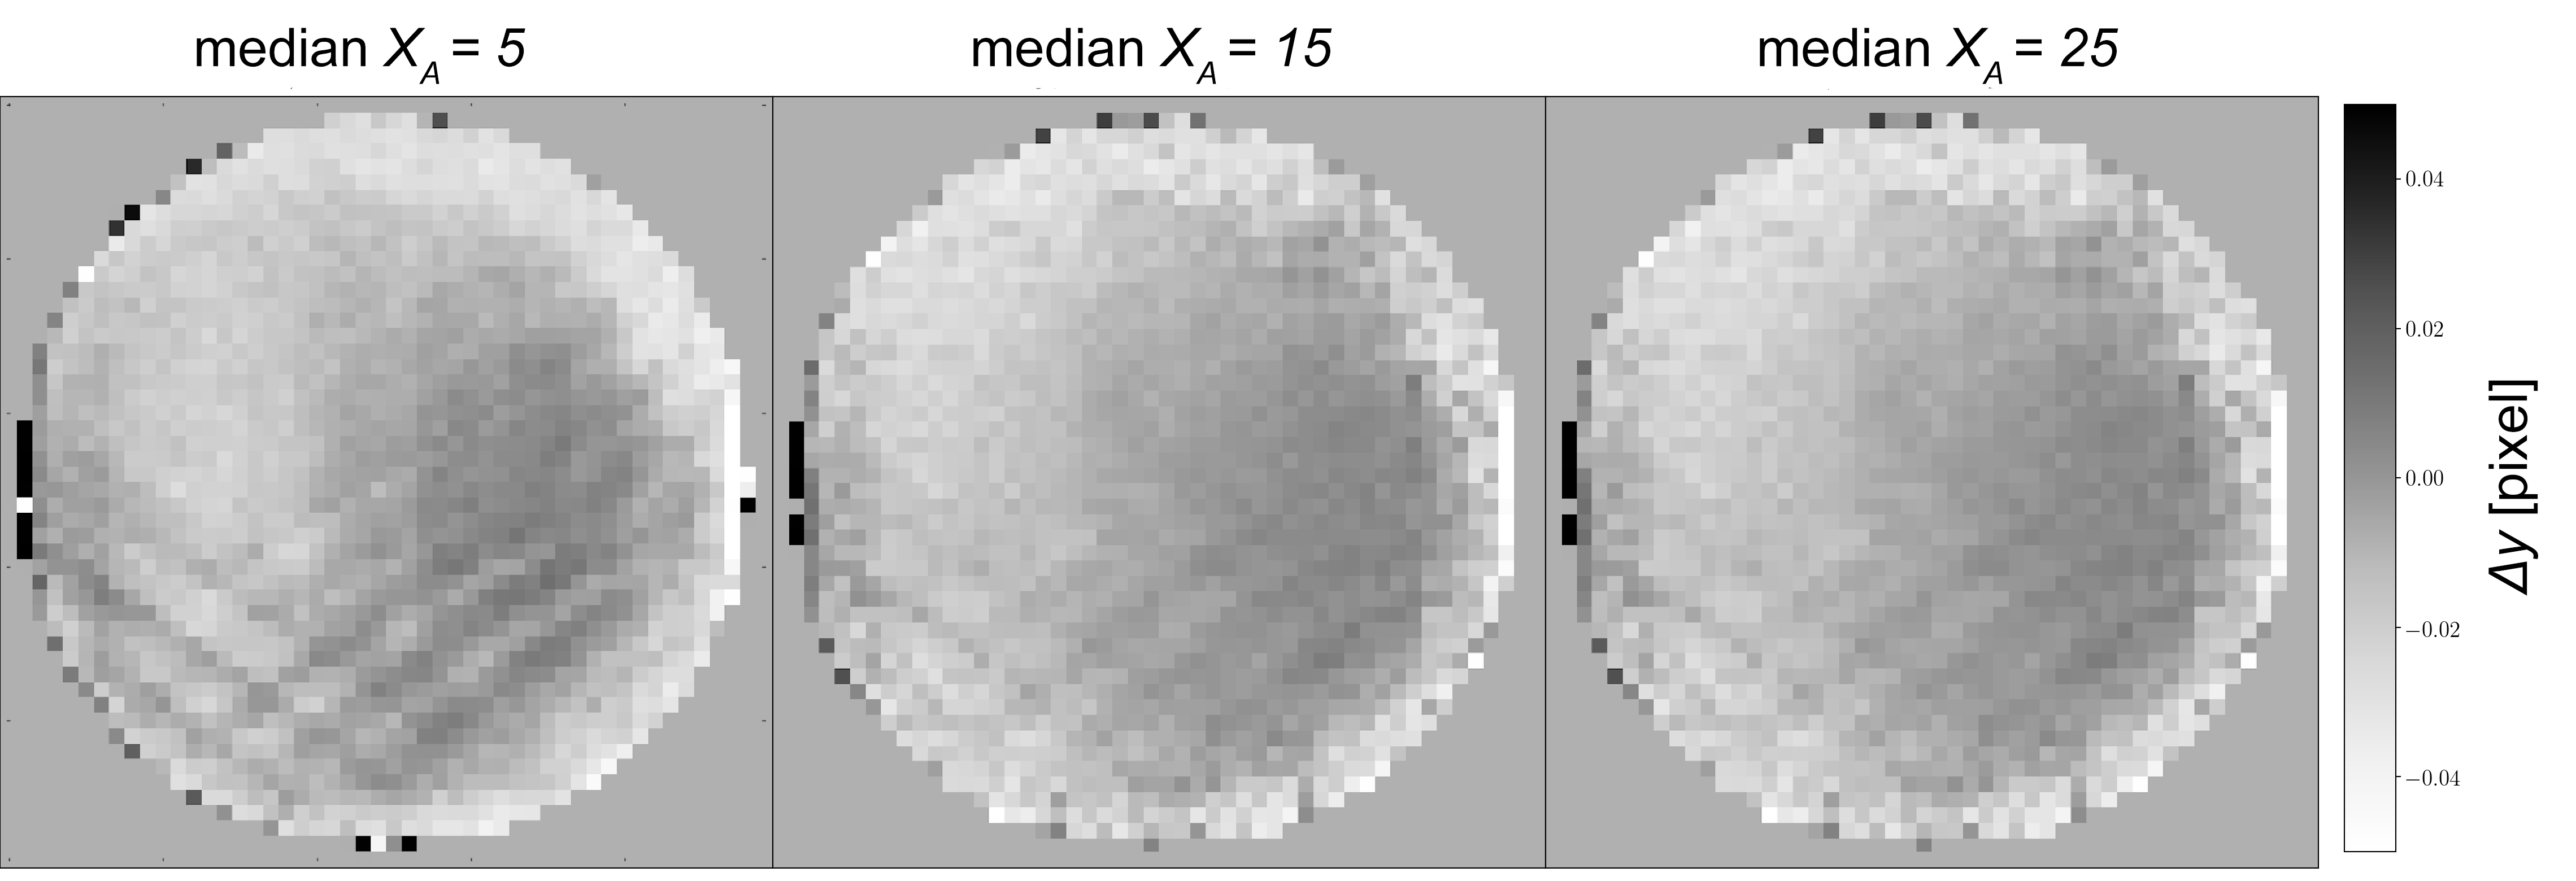
\includegraphics[width=0.95\textwidth]{figures/gs/xa-y-new}
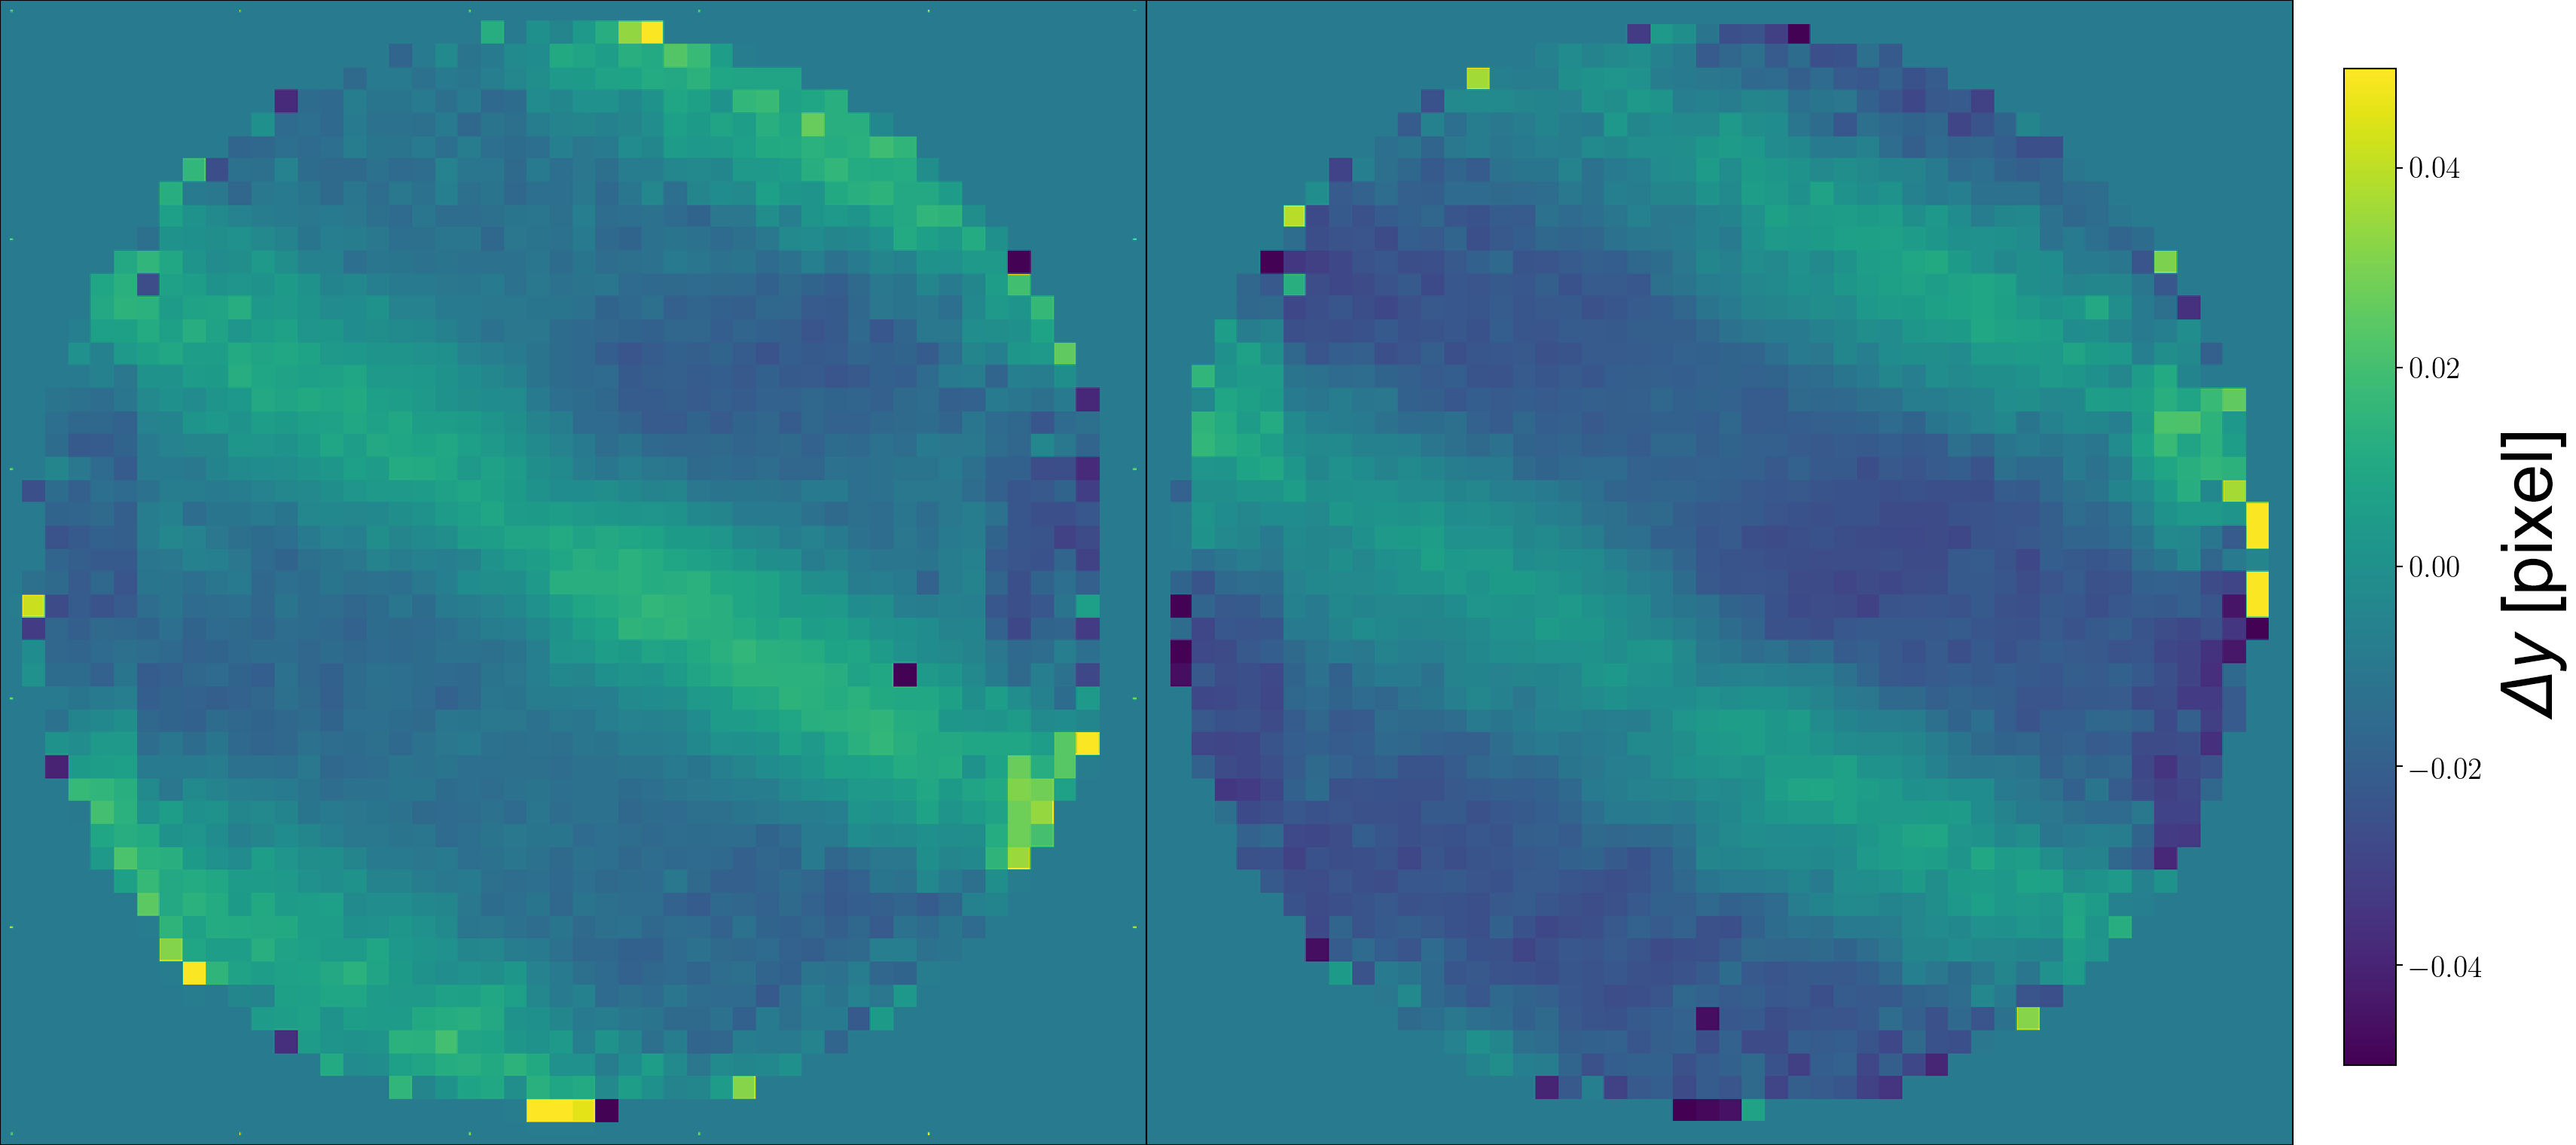
\includegraphics[width=0.6\textwidth]{figures/gs/dif-xa-y-new}

\end{center}
\caption[The calibrated distortion map with different $X_A$]{%
  \label{distortion_xa}
  Distortion-maps of photons with different $X_A$.
  \emph{First row:} Distortion-map in x direction.
  From left to right, the $X_A$ value of photons increases.
  \emph{Second row:} Difference between distortion-maps in the first row.
  \emph{Third row:} Distortion-map in y direction.
  From left to right, the $X_A$ value of photons increases.
  \emph{Forth row:} Difference between distortion-maps in the third row.
  There is a periodic pattern in difference over the detector, which is expected to account for the phases of the coarse clock.
  }
\end{figure}

\begin{figure}[p]
\begin{center}
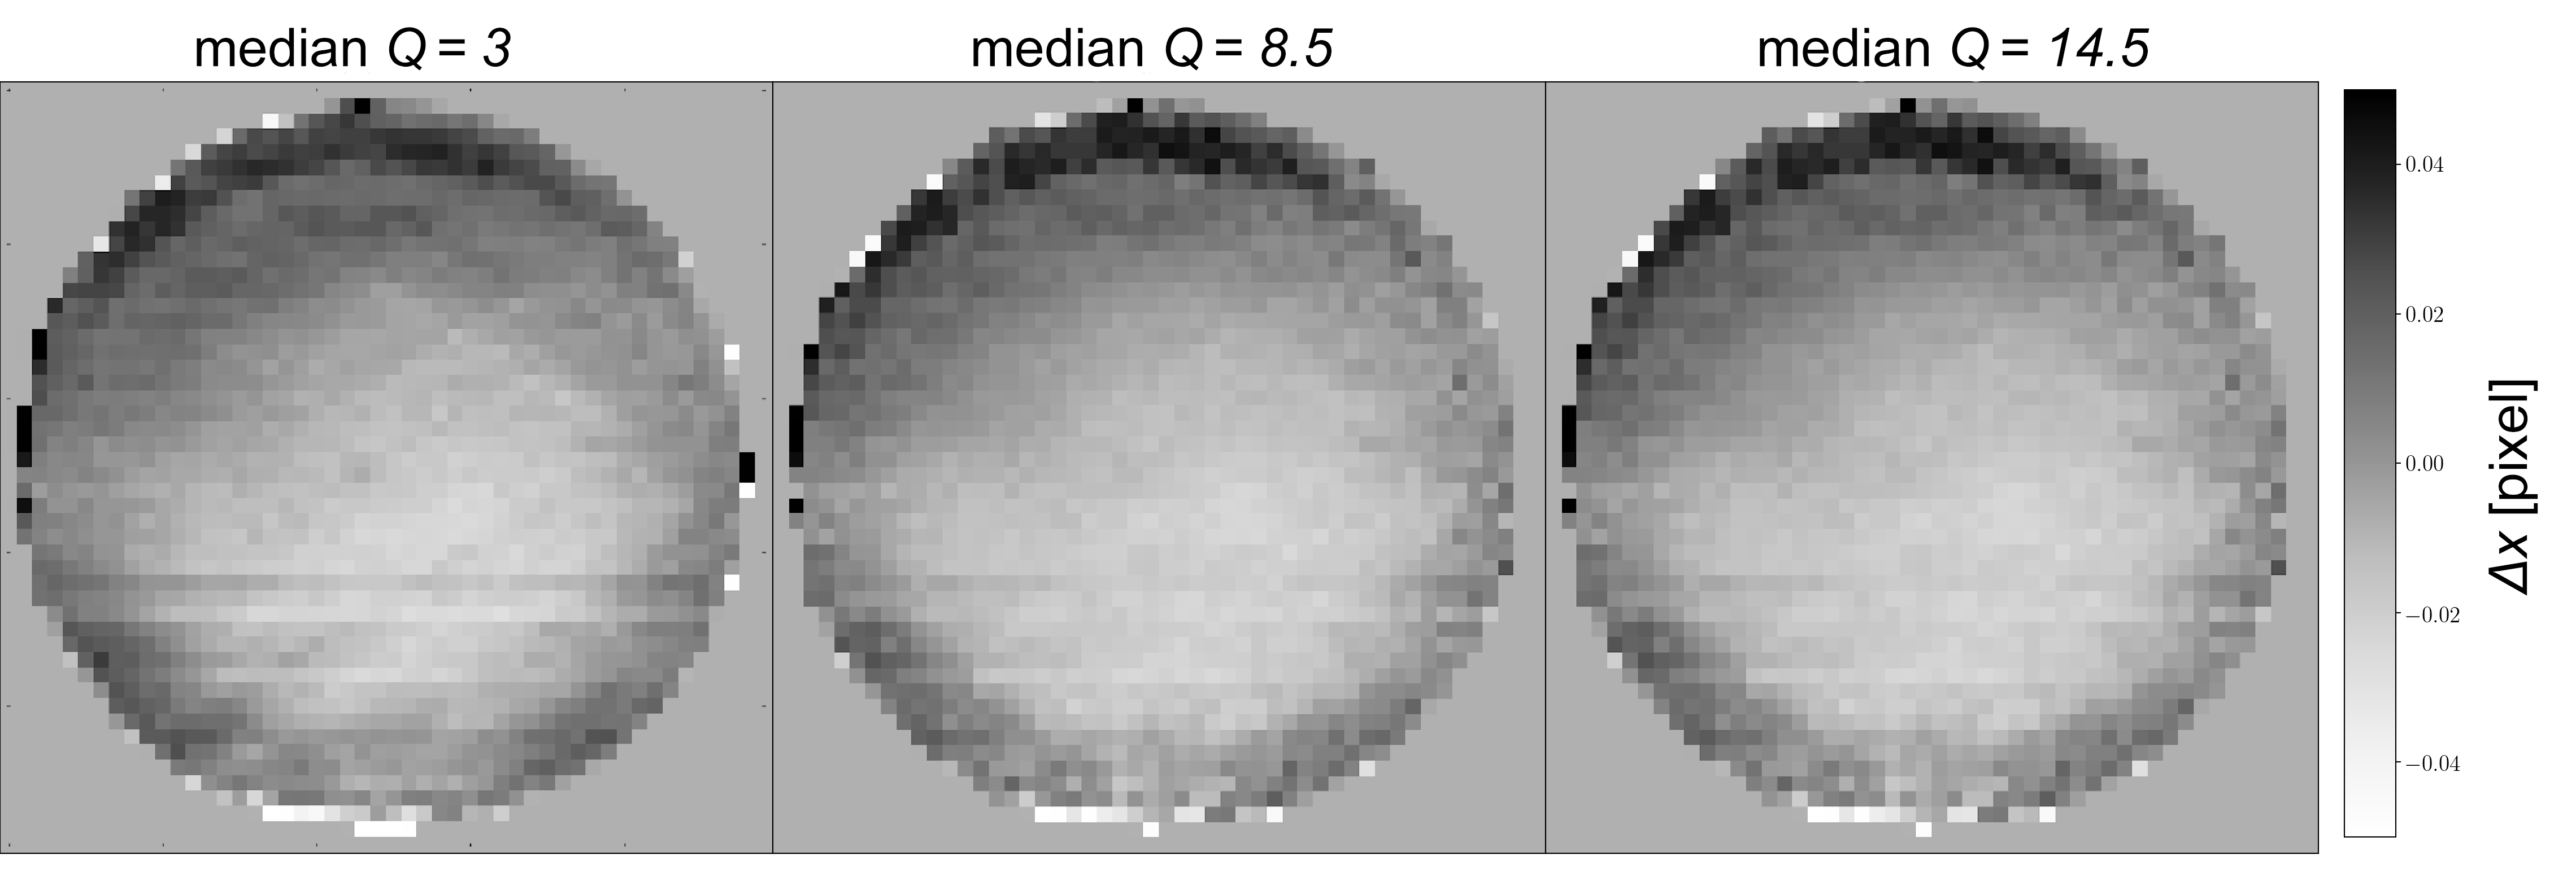
\includegraphics[width=0.95\textwidth]{figures/gs/q-x-new}
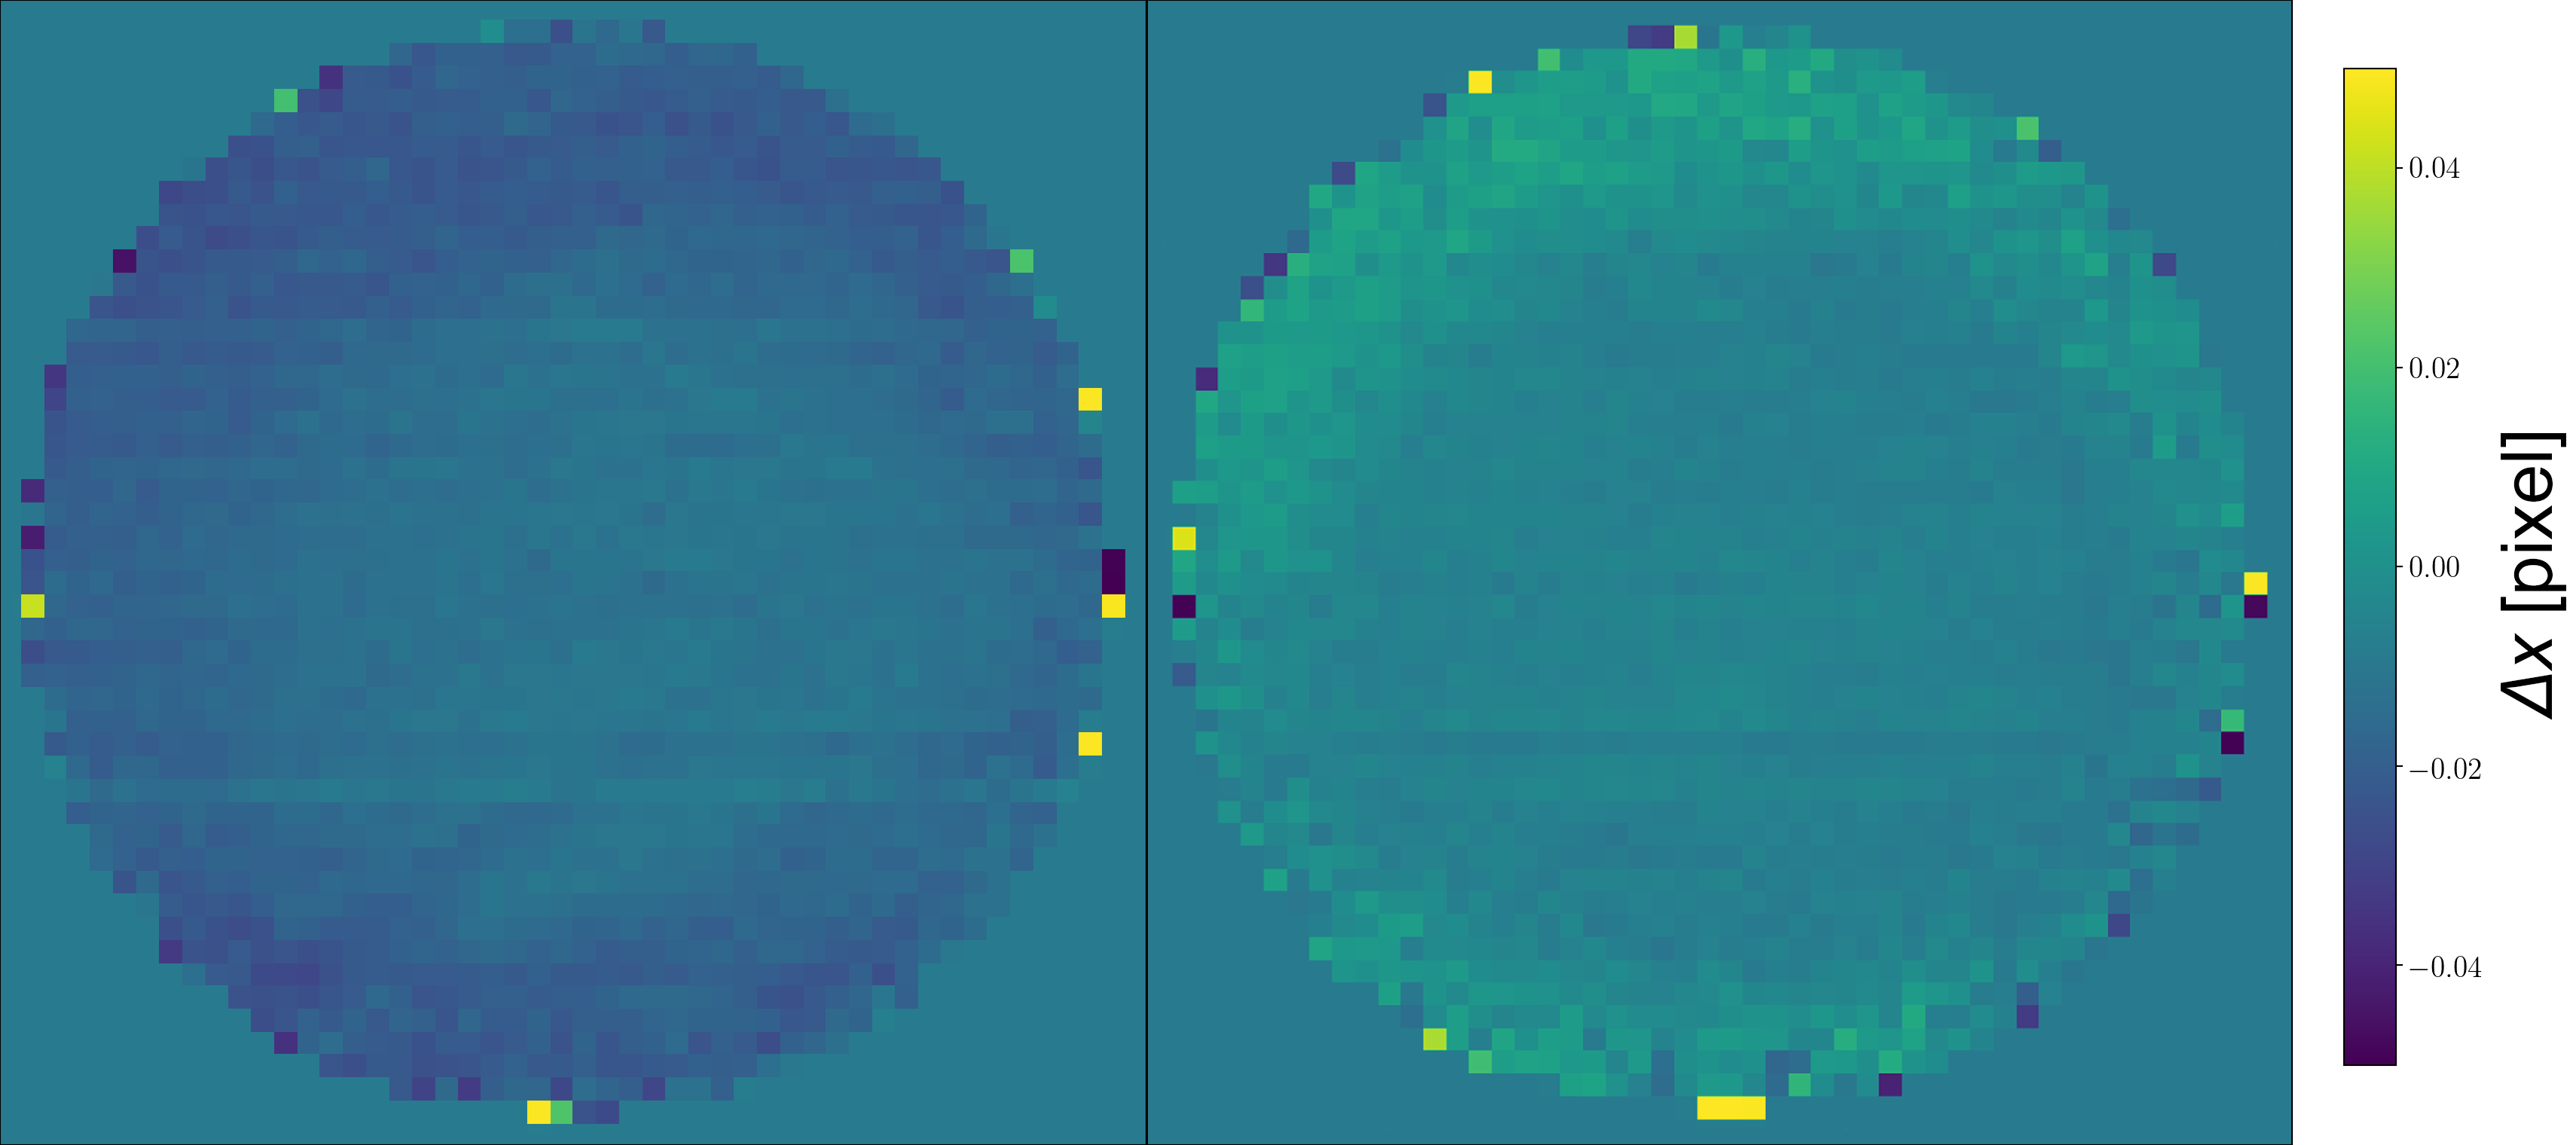
\includegraphics[width=0.6\textwidth]{figures/gs/dif-q-x-new}
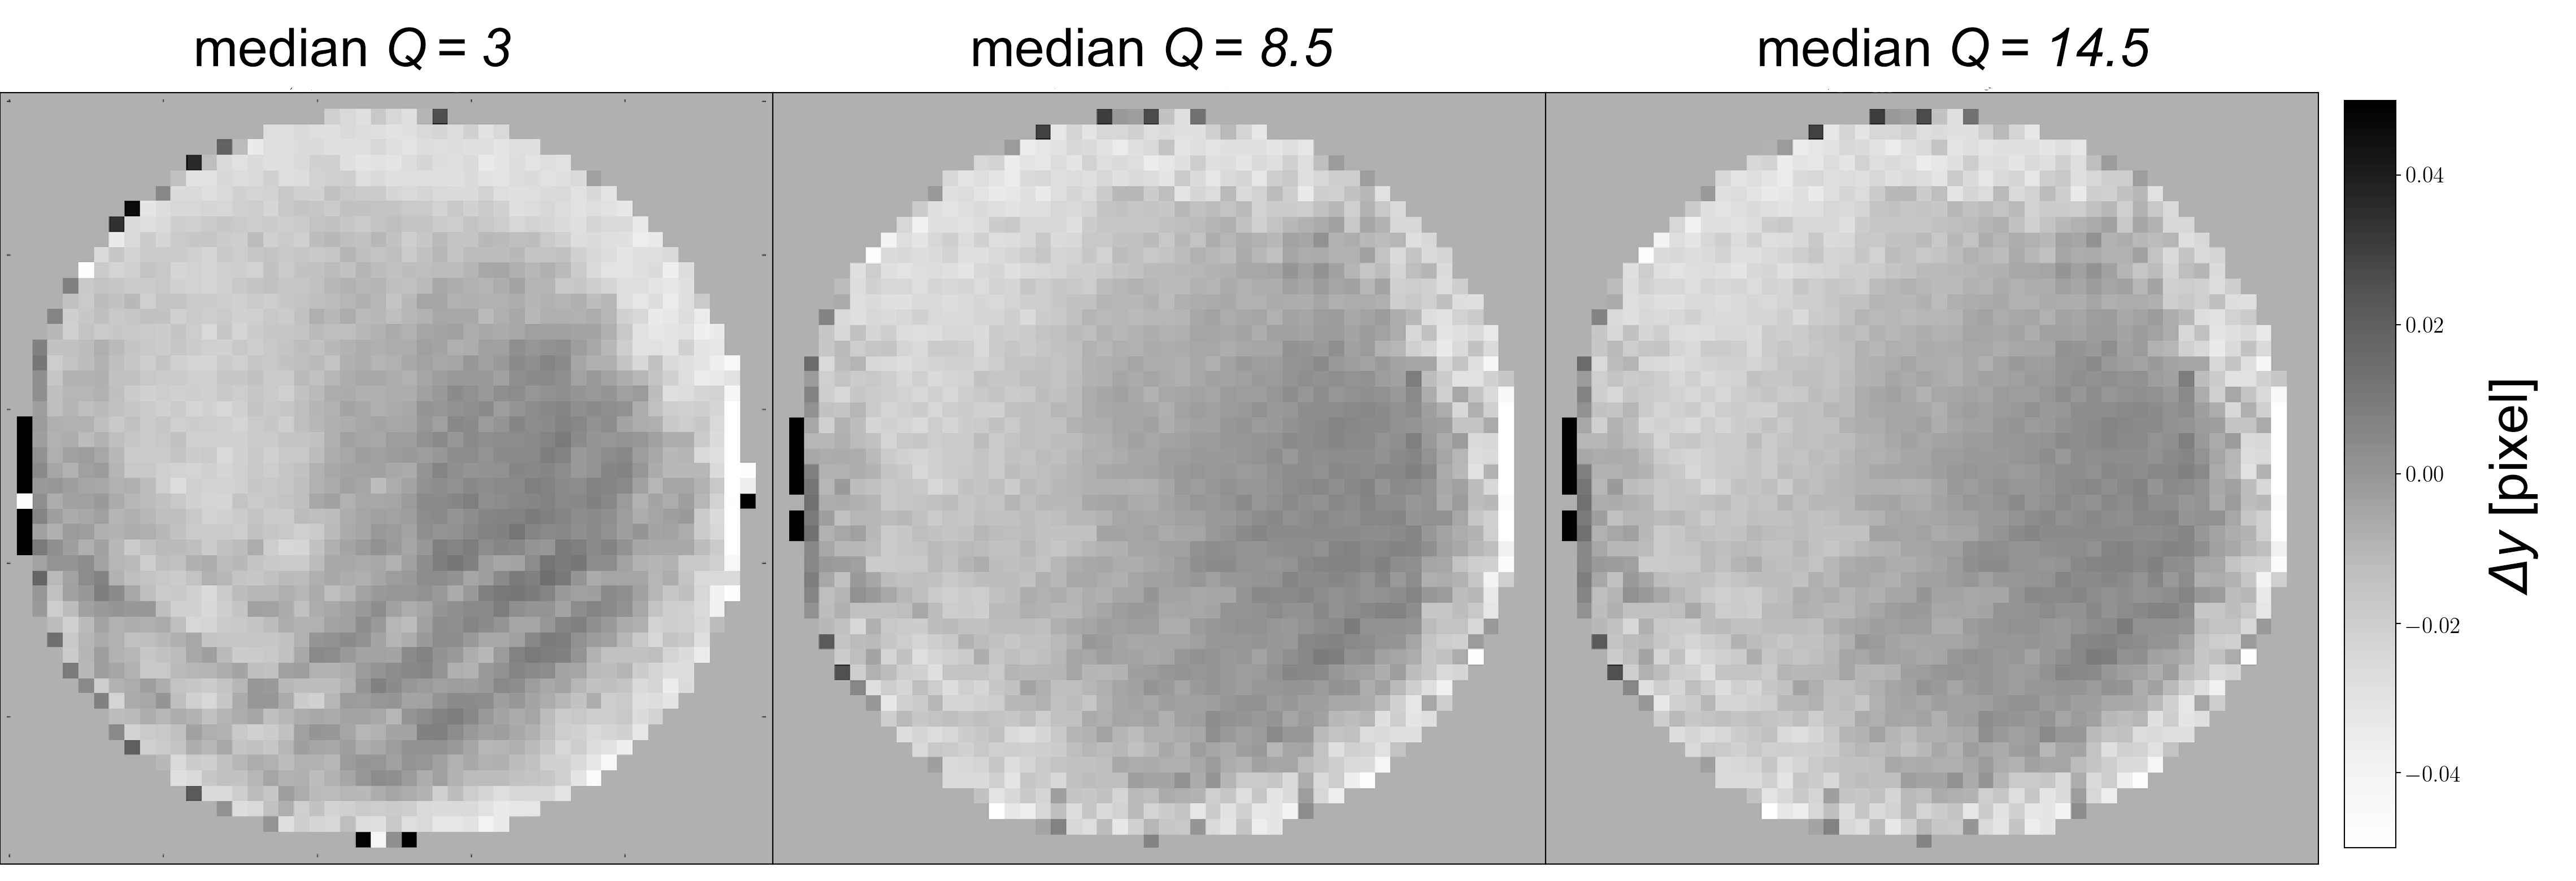
\includegraphics[width=0.95\textwidth]{figures/gs/q-y-new}
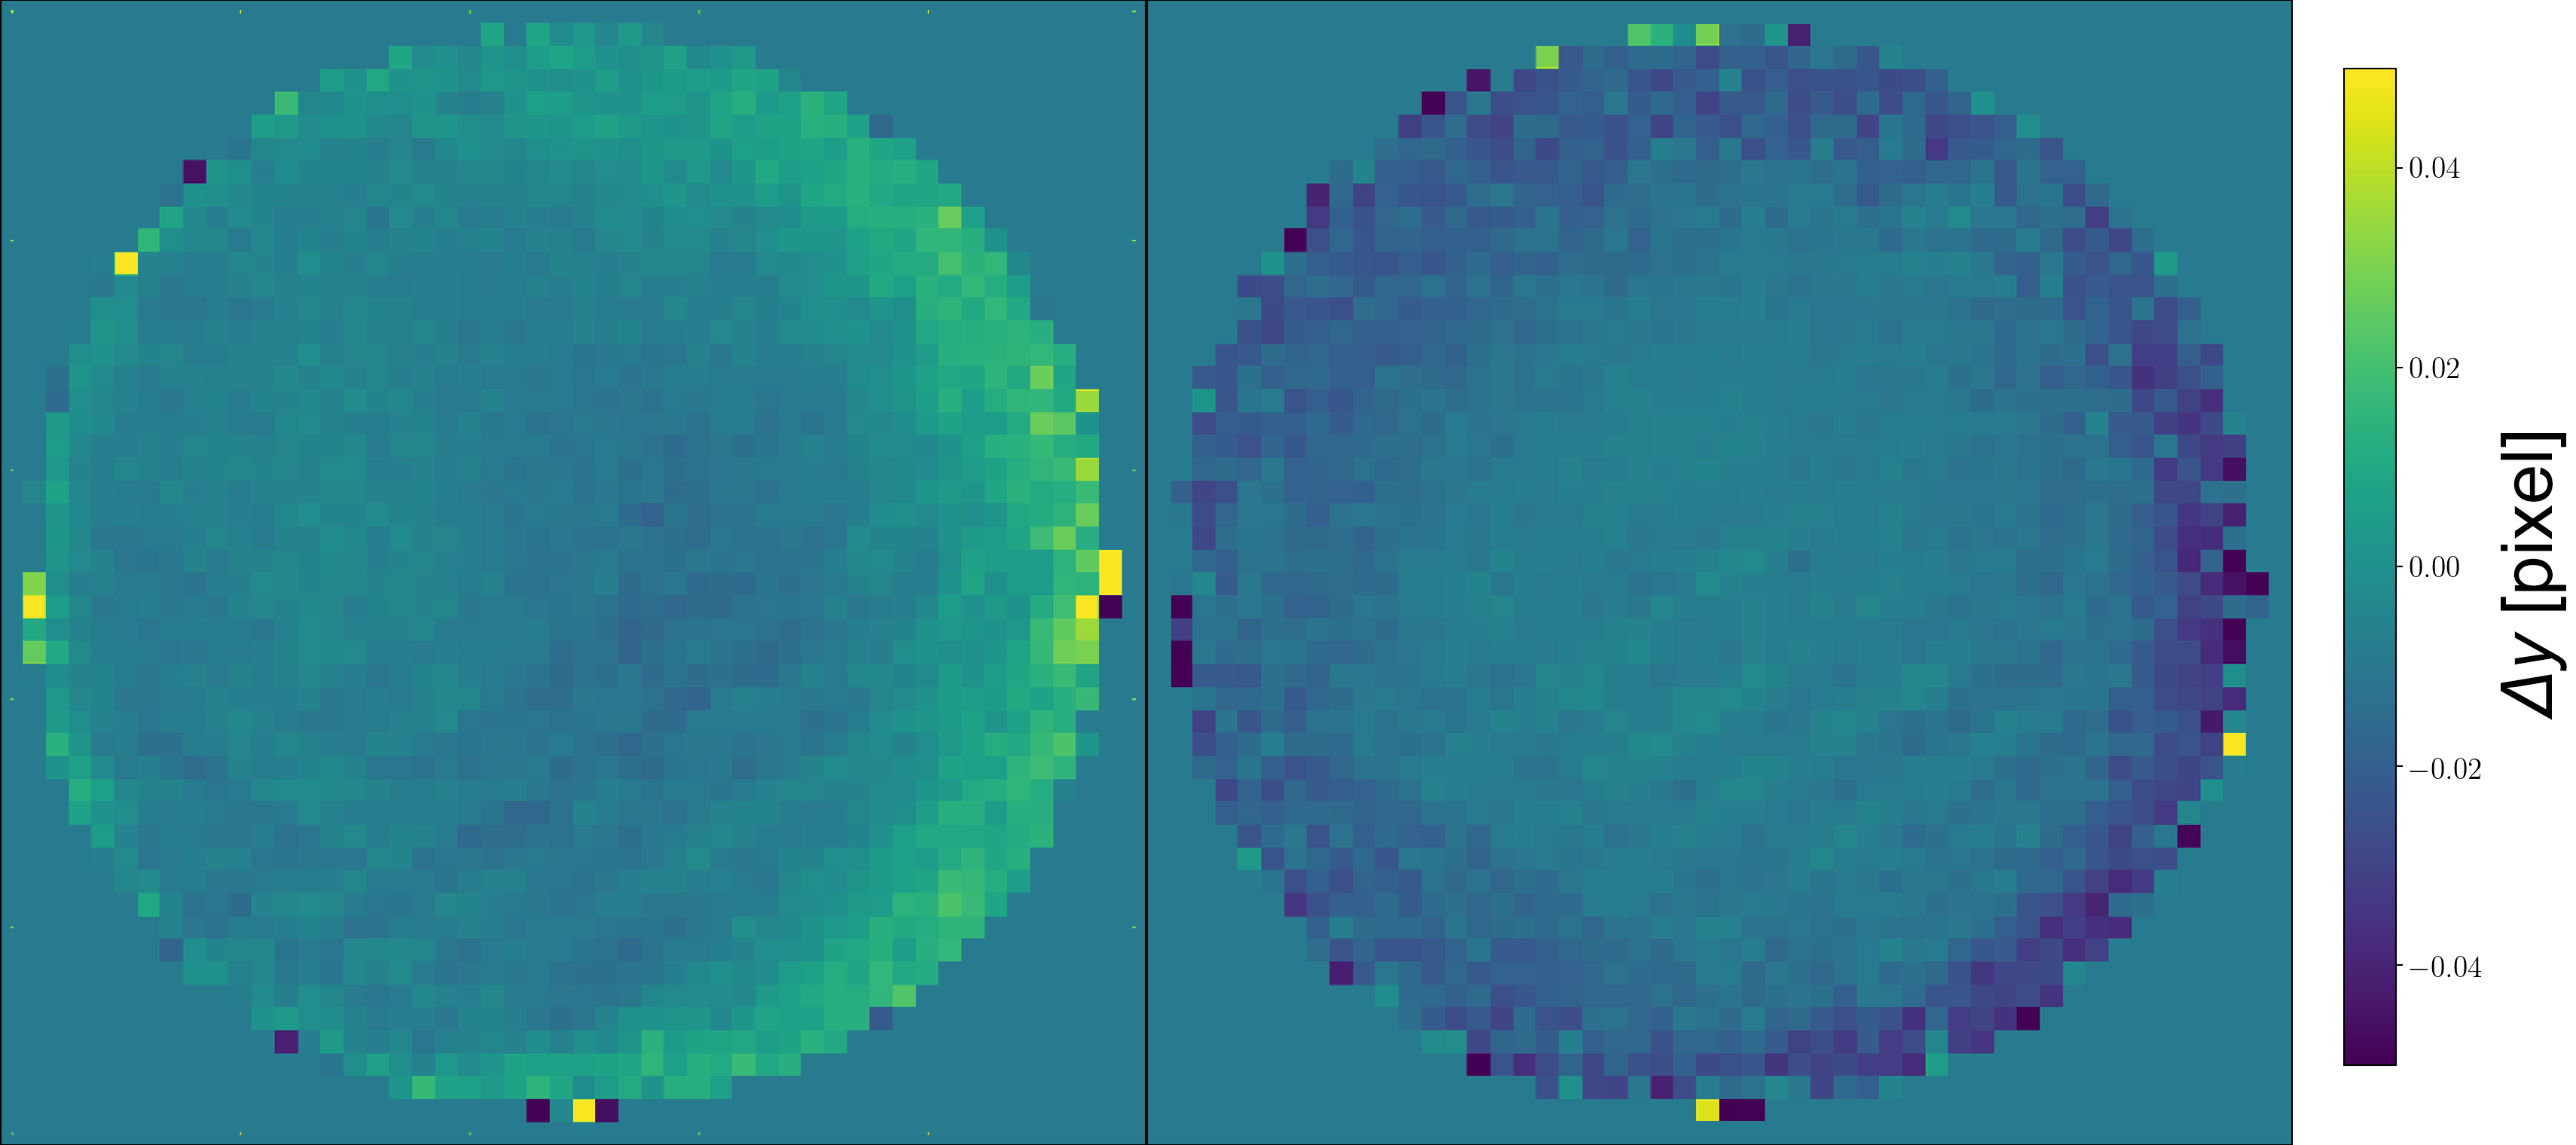
\includegraphics[width=0.6\textwidth]{figures/gs/dif-q-y-new}

\end{center}
\caption[The calibrated distortion map with different Q]{%
  \label{distortion_q}
  Distortion-maps of photons with different Q.
  \emph{First row:} Distortion-maps in x direction. 
  From left to right, the Q value of photons increases.
  \emph{Second row:} Difference between distortion-maps in the first row.
  \emph{Third row:} Distortion-map in y direction.
  From left to right, the Q value of photons increases.
  \emph{Forth row:} Difference between distortion-maps in the third row.
  }
\end{figure}


\section{Sensitivity map}
\label{sm}
To precisely construct the intensity map, the effective exposure time needs to be measured. 
Since the response function of the detector is not uniform, the sensitivity map is required to scale the effective exposure time for different pixels.
The original pipeline sensitivity map is not appropriate to be used in the calibration due to the following reasons:
\begin{enumerate}
\item The pipeline sensitivity map was constructed using ground measurements of the system throughput, which may not capture the finer details of the instrument response.
\item The \cause\ observation was conducted in the very late stage of the mission, so the response of detector could have changed during the telescope lifetime.
\item The Galactic Plane data used in this paper were observed in high count rate/high background regions of the sky.  
Therefore the additional cuts (photons with $Q<=5$) described in section \ref{data} is required to avoid certain effects from the high count rate. 
However the photon Q value distribution over the detector is not uniform.
Fig.~\ref{qcut} shows the ratio of the remaining photons after the cut.
There are more photons cut around the edge than in the center of the detector, which changed the effective response correspondingly.
\end{enumerate}

Thanks to the observation strategy in \scanmode, each source samples a cord across the entire detector. 
If every star is assumed to be constant in brightness, the count of photons in pixel $(x,y)$ from star $i$, $C_{i,x,y}$ can be modelled as:
\begin{eqnarray}
C_{i,x,y} &=& I_{i}f_{x,y}T_{i,x,y}
\end{eqnarray}
where $I_{i}$ is the brightness of star $i$. 
$f_{x,y}$ is the sensitivity of pixel $(x,y)$.
$T_{i,x,y}$ is the exposure time of star $i$ at pixel $(x,y)$.

Starting from the original pipeline sensitivity map $f_{x,y}^{0}$, the sensitivity map is updated iteratively by the following equations:
\begin{eqnarray}
I_{i}^{n} &=& \frac{\sum_{x,y}C_{i,x,y}}{\sum_{x,y} f_{x,y}^{n} T_{i,x,y}} \\
f_{x,y}^{n+1} &=& \frac{\sum_{i}C_{i,x,y}}{\sum_{i} I_{i}^{n} T_{i,x,y}}
\end{eqnarray}

Fig.~\ref{flat} shows the comparison between the pipeline sensitivity map and the measured sensitivity map.
The measured sensitivity map reproduced some of the bad spots in the original map, while has an overall lower response on the edge, which is due to the cut of the photon list.

However, the relative sensitivity of pixels will also vary as a function of the overall local photon countrate.
Fig.~\ref{countrate} compares the photometry from the \cause\ data (this paper) and the \asc\ in regions with different overall intensity.
The detail of the photometry will be discussed in the catalog paper (Mohammed et al., in prep).
The photometry in regions with moderate countrate (second row) agrees well with the \asc, since most stars used to measure the sensitivity map reside in these regions.
In comparison, photometry in regions with low or high overall intensity (first and third row) consists consistent systematics that in low countrate region, the photometry is overestimated in the edge, while in high countrate region, it is underestimated in the edge.
These systematics are probably caused by the various photon Q value distribution over the detector when exposed to different countrate regions.
Therefore to better calibrate the effective exposure of the image, the sensitivity map should be measured as a function of the photon countrate.
Fig.~\ref{flat-profile} shows the profile plots of the sensitivity maps constructed by photons from regions with different photon countrates.
The difference of the sensitivity maps account for the systematics shown in Fig.~\ref{countrate}.

\begin{figure}[p]
\begin{center}
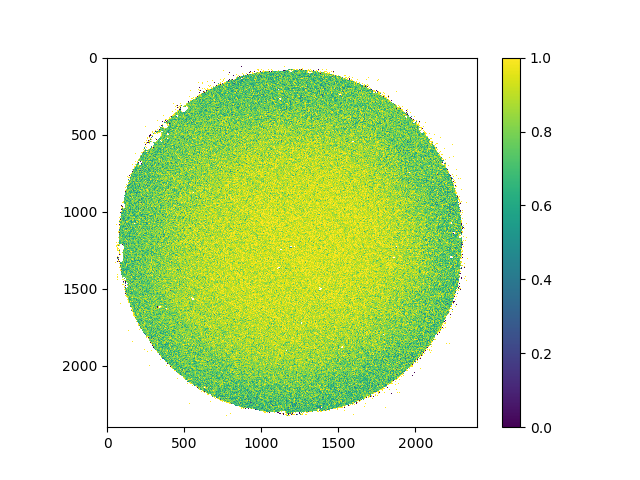
\includegraphics[width=0.8\textwidth]{figures/gs/q50}
\end{center}
\caption[The ratio of the remaining photons to the total after cutting the photons with $Q<=5$]{
  \label{qcut}
  The ratio of the remaining photons to the total after cutting the photons with $Q<=5$.
  There are more photons cut around the edge than in the center of the detector, which leads to a very different effective sensitivity map from the original pipeline.
}
\end{figure}

\begin{figure}[p]
\begin{center}
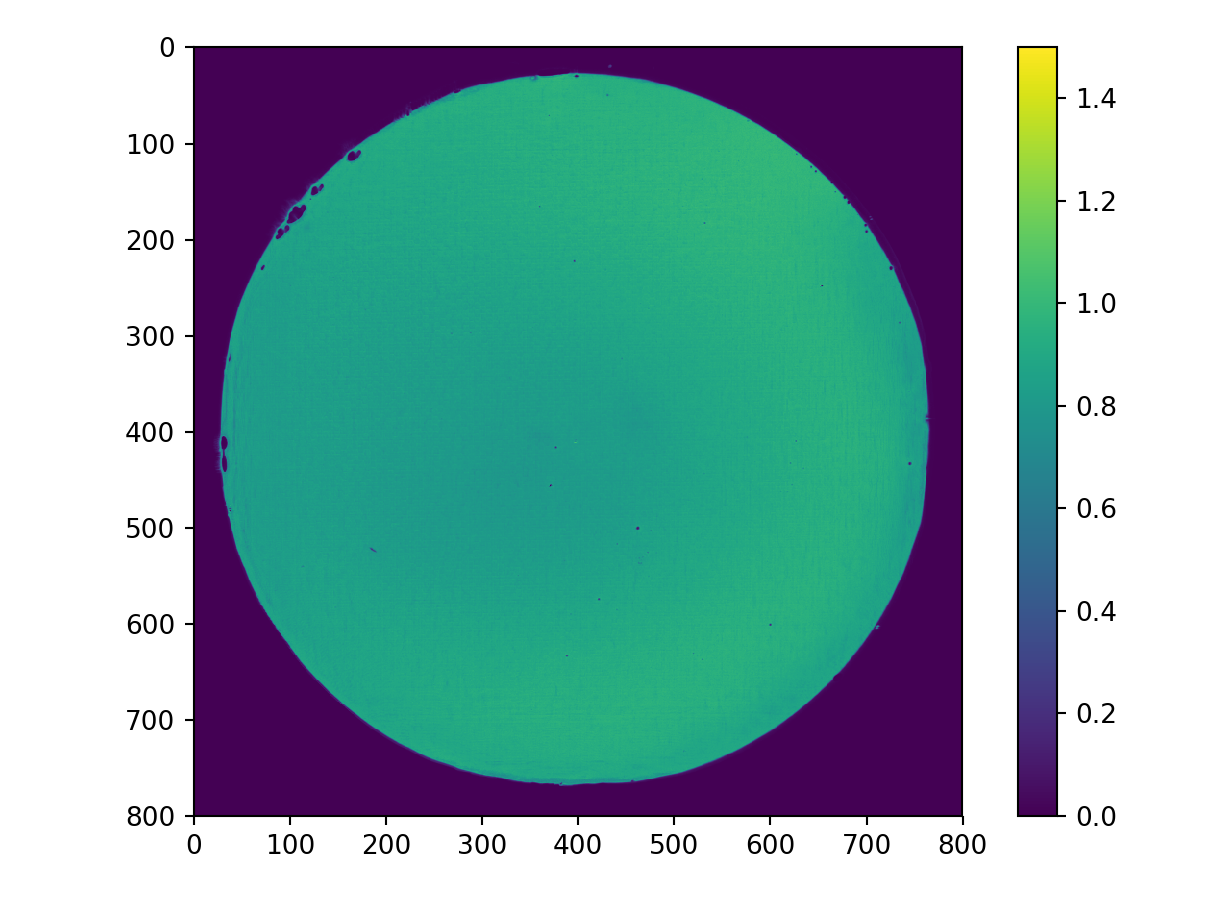
\includegraphics[width=0.48\textwidth]{figures/gs/flato}
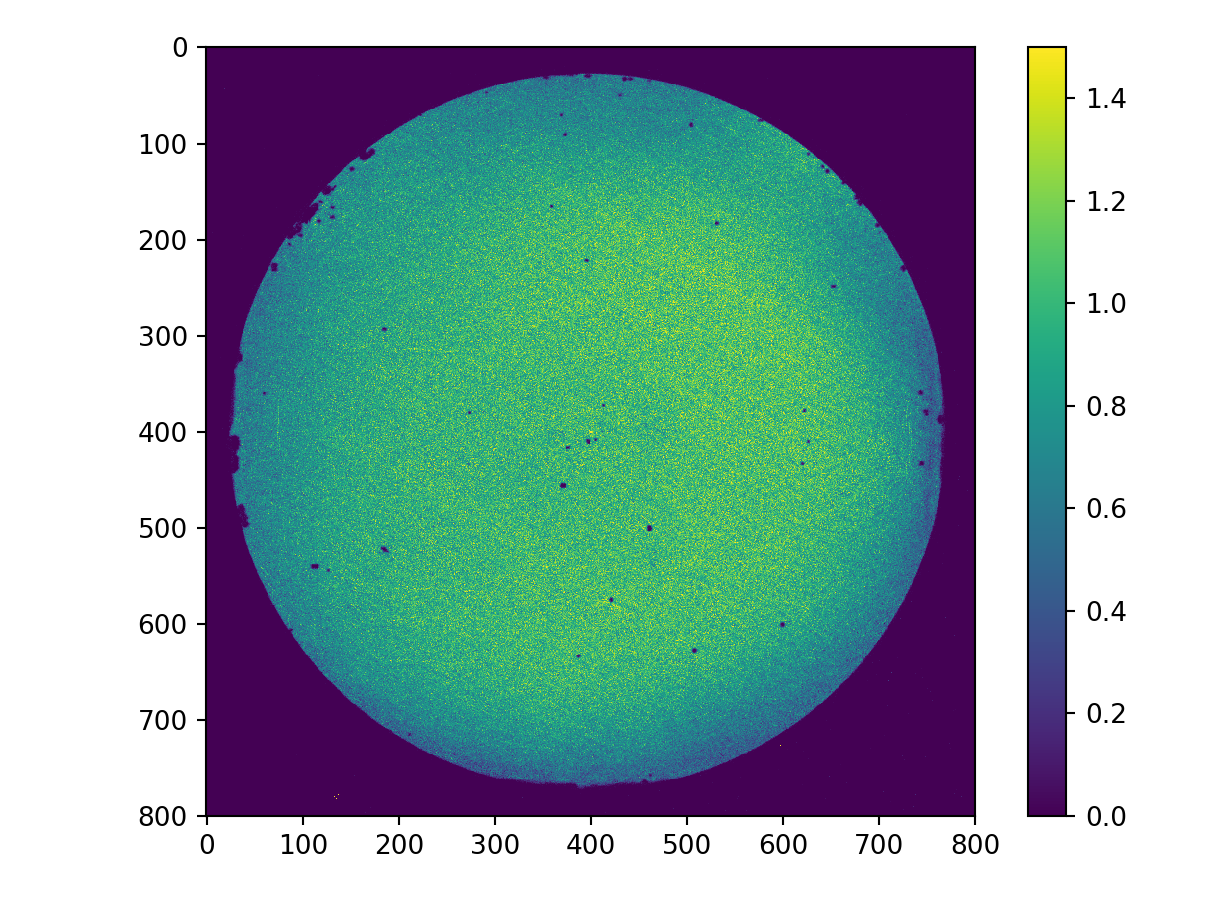
\includegraphics[width=0.48\textwidth]{figures/gs/flat}
\end{center}
\caption[Comparison between pipeline and measured sensitivity map]{
  \label{flat}
  Comparison between pipeline and measured sensitivity map.
  \emph{Left:} Pipeline sensitivity map;
  \emph{Right:} The converged sensitivity map.
  The measured sensitivity map reproduced some of the bad spots in the original map, while has an overall lower response on the edge, which is due to the cut of the photon list.
}
\end{figure}

\begin{figure}[p]
\begin{center}
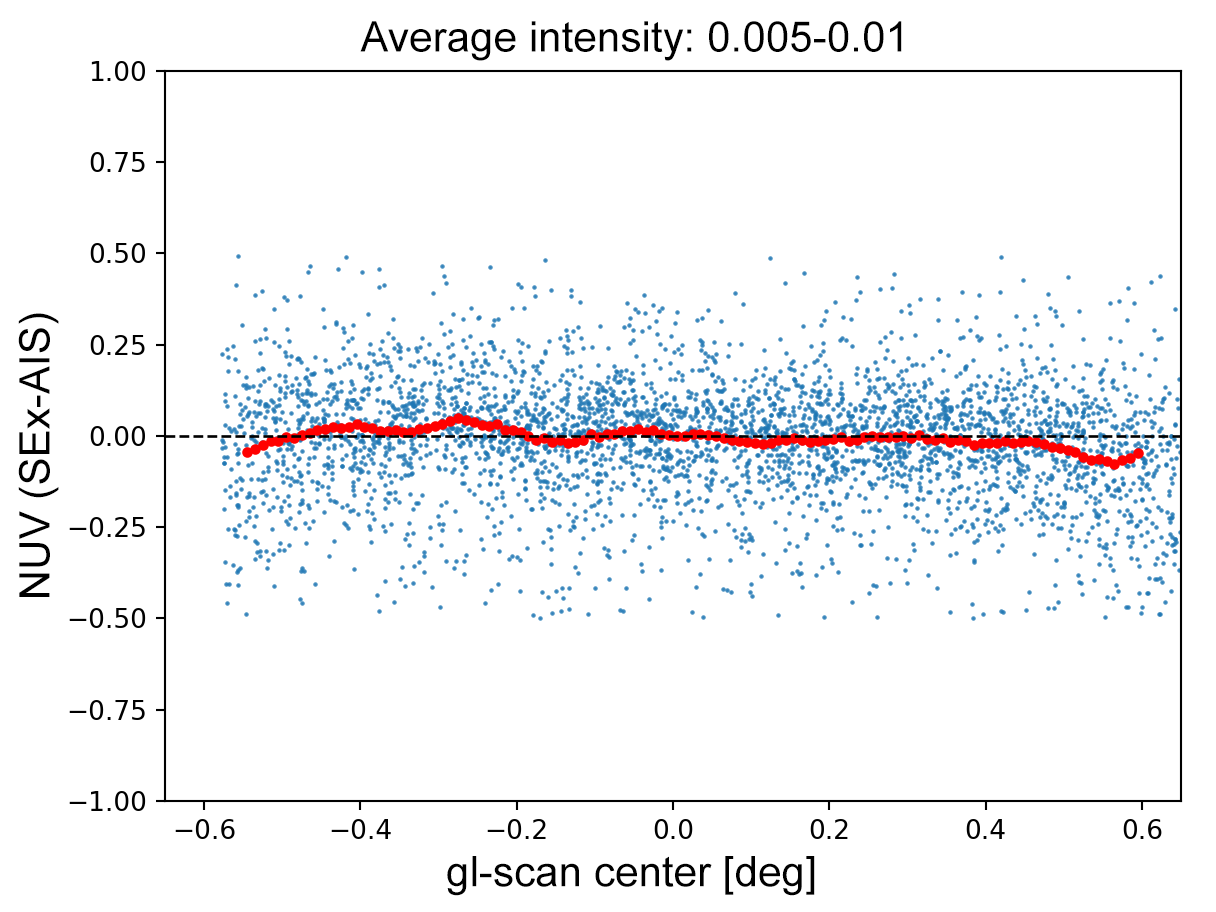
\includegraphics[width=0.48\textwidth]{figures/gs/cr1-new}
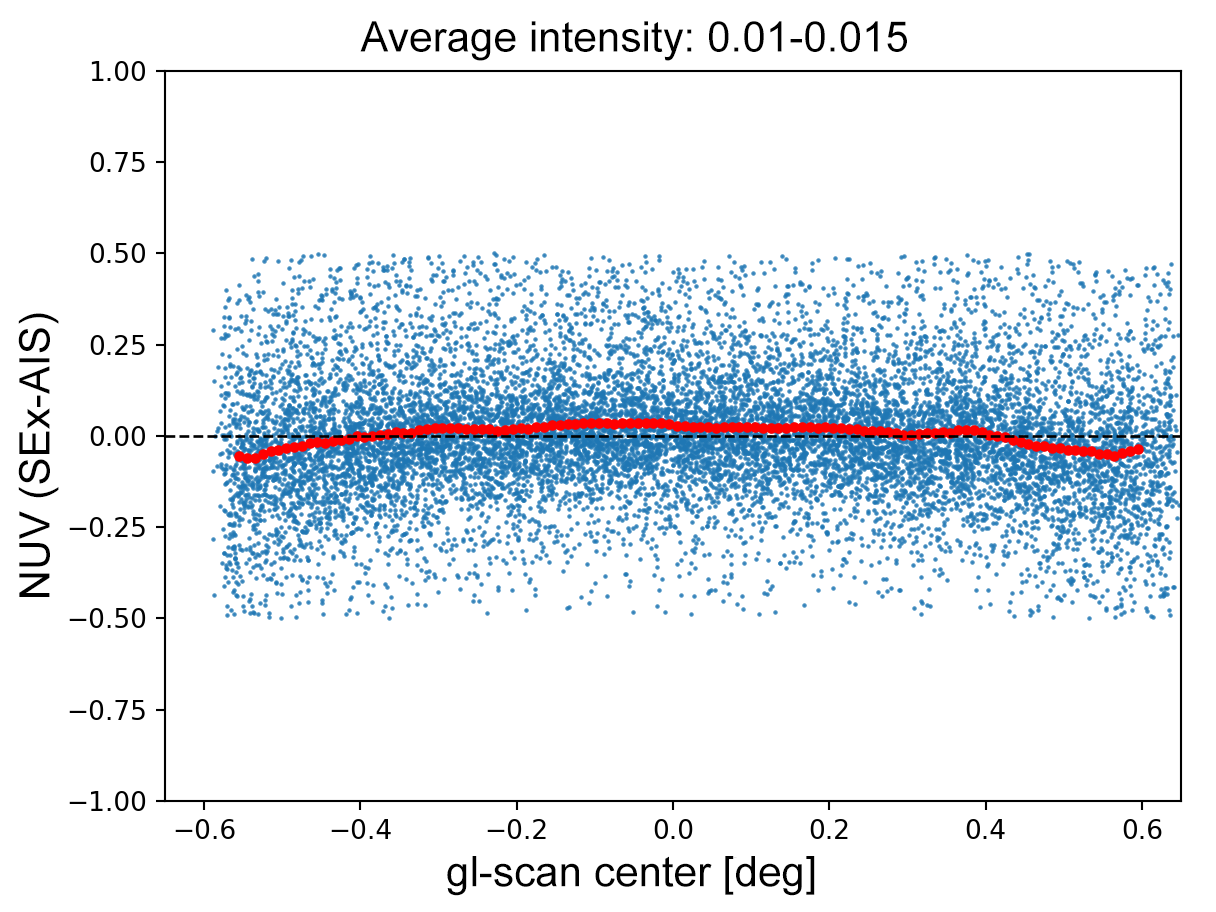
\includegraphics[width=0.48\textwidth]{figures/gs/cr2-new}
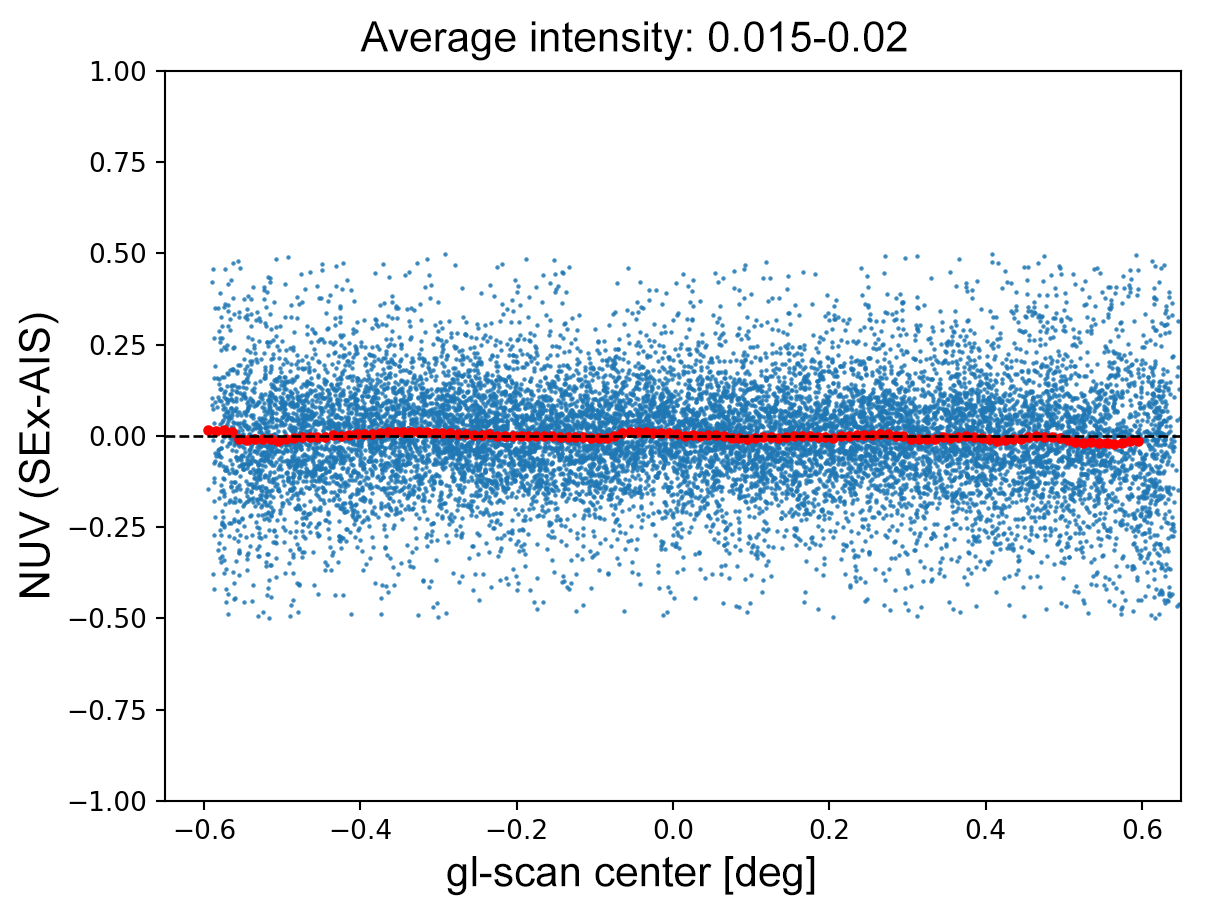
\includegraphics[width=0.48\textwidth]{figures/gs/cr3-new}
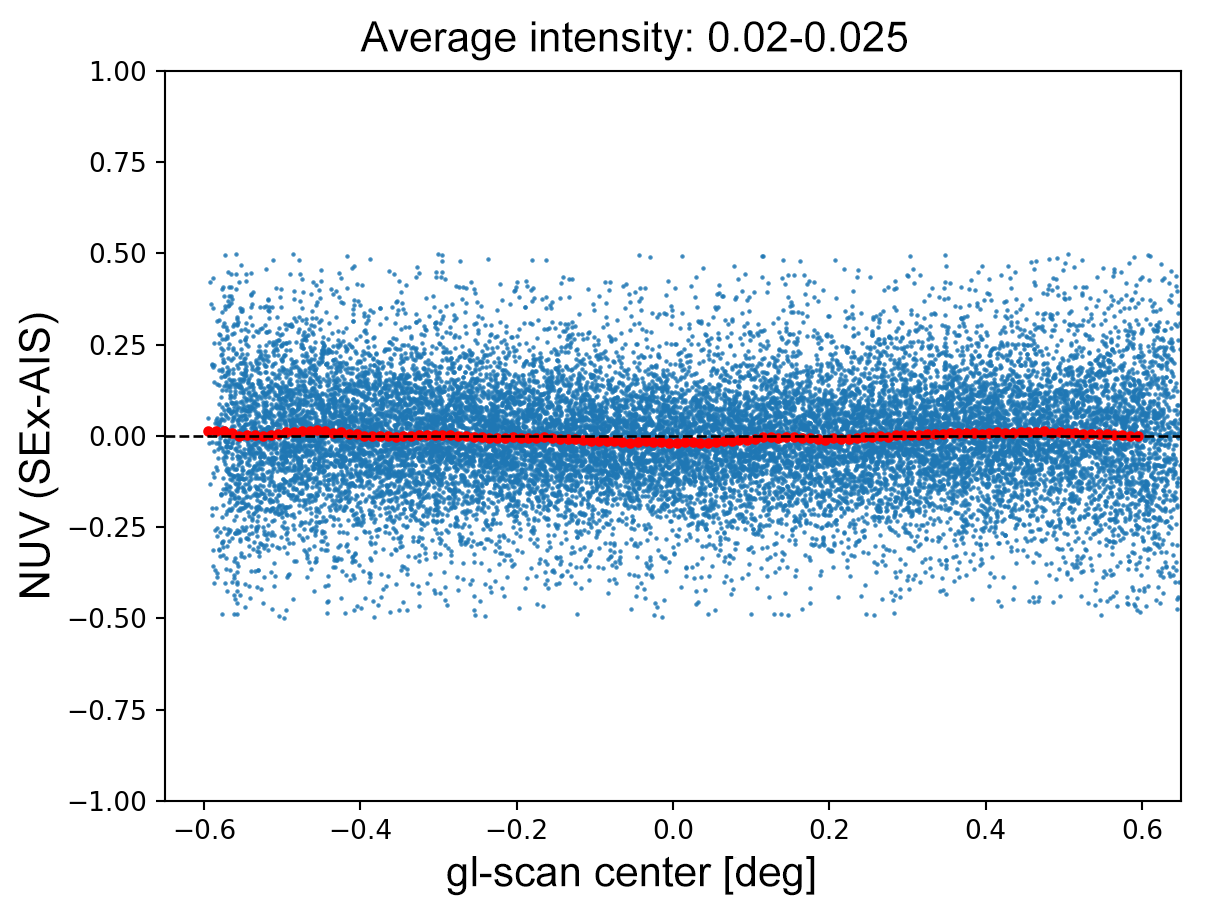
\includegraphics[width=0.48\textwidth]{figures/gs/cr4-new}
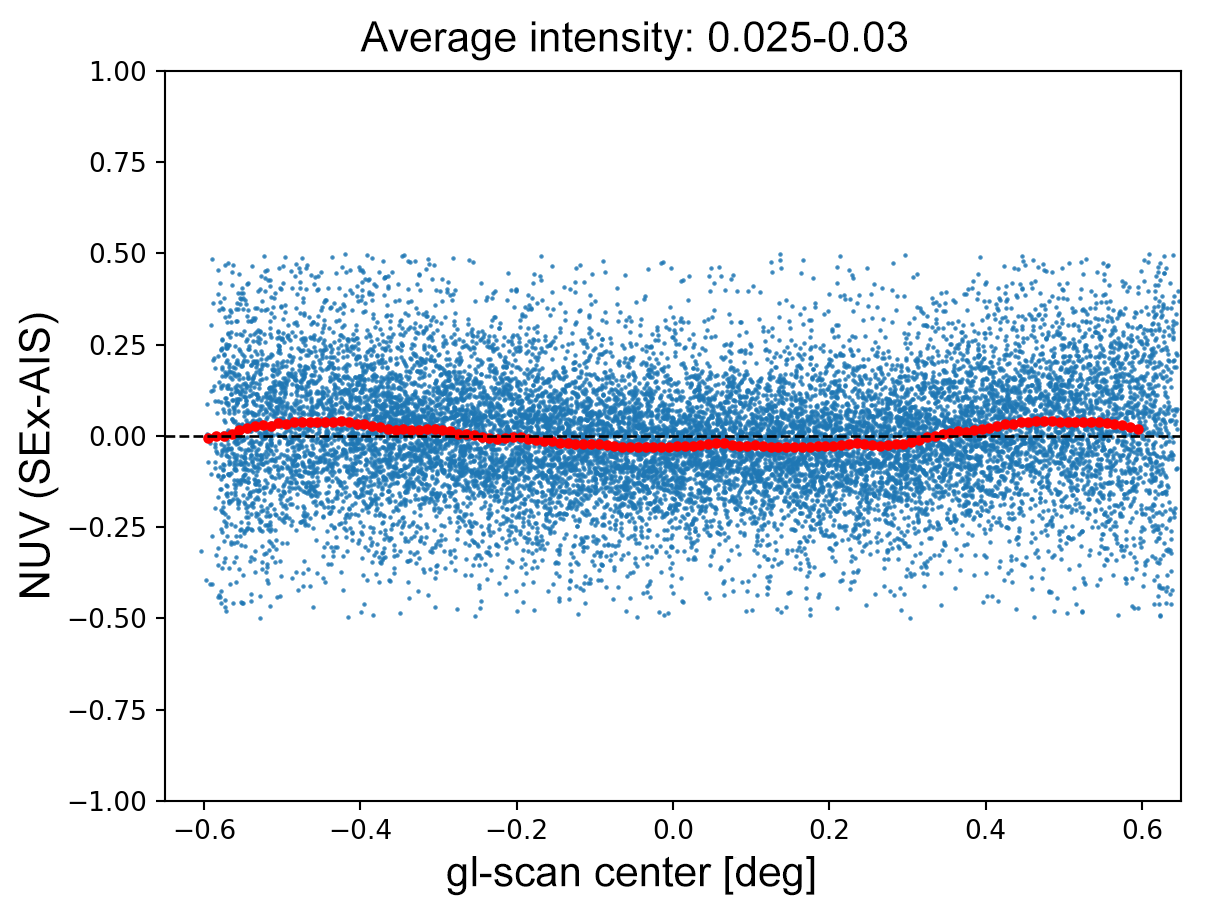
\includegraphics[width=0.48\textwidth]{figures/gs/cr5-new}
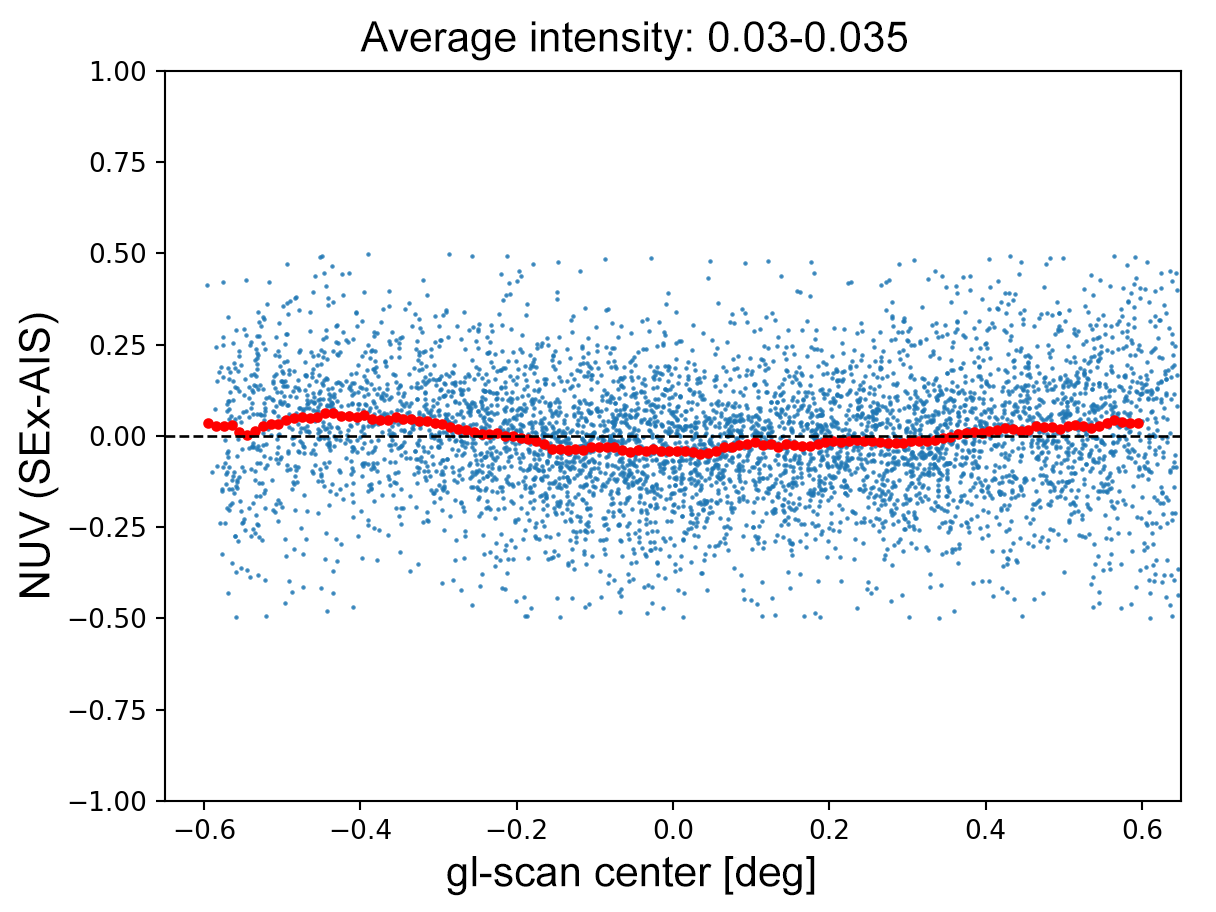
\includegraphics[width=0.48\textwidth]{figures/gs/cr6-new}
\end{center}
\caption[Matched sources comparison in regions with different count rates]{
  \label{countrate}
  Magnitude difference of matched sources between the \cause\ data (this paper) and the \asc\ as a function of radial distance from the detector center. 
  The red line shows the median difference.
  These six plots show the relation in regions of the sky with different overall intensity.
  The photometry in regions with moderate countrate (second row) agrees well with the \asc.
  In comparison, in low countrate region (first row), the photometry is overestimated in the edge of the detector, while in high countrate region (third row), the photometry is underestimated in the edge.
}
\end{figure}

\begin{figure}[p]
\begin{center}
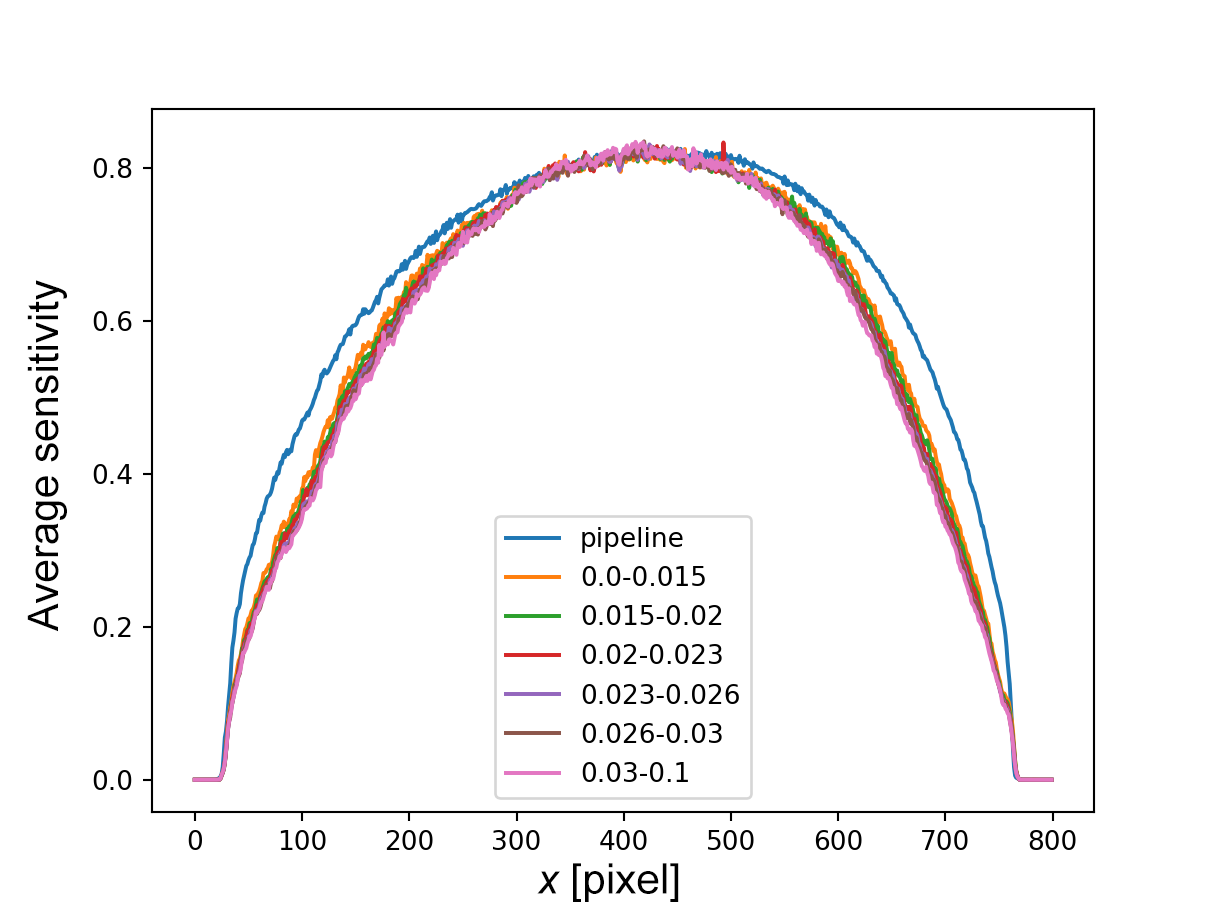
\includegraphics[width=0.48\textwidth]{figures/gs/profile_x-new}
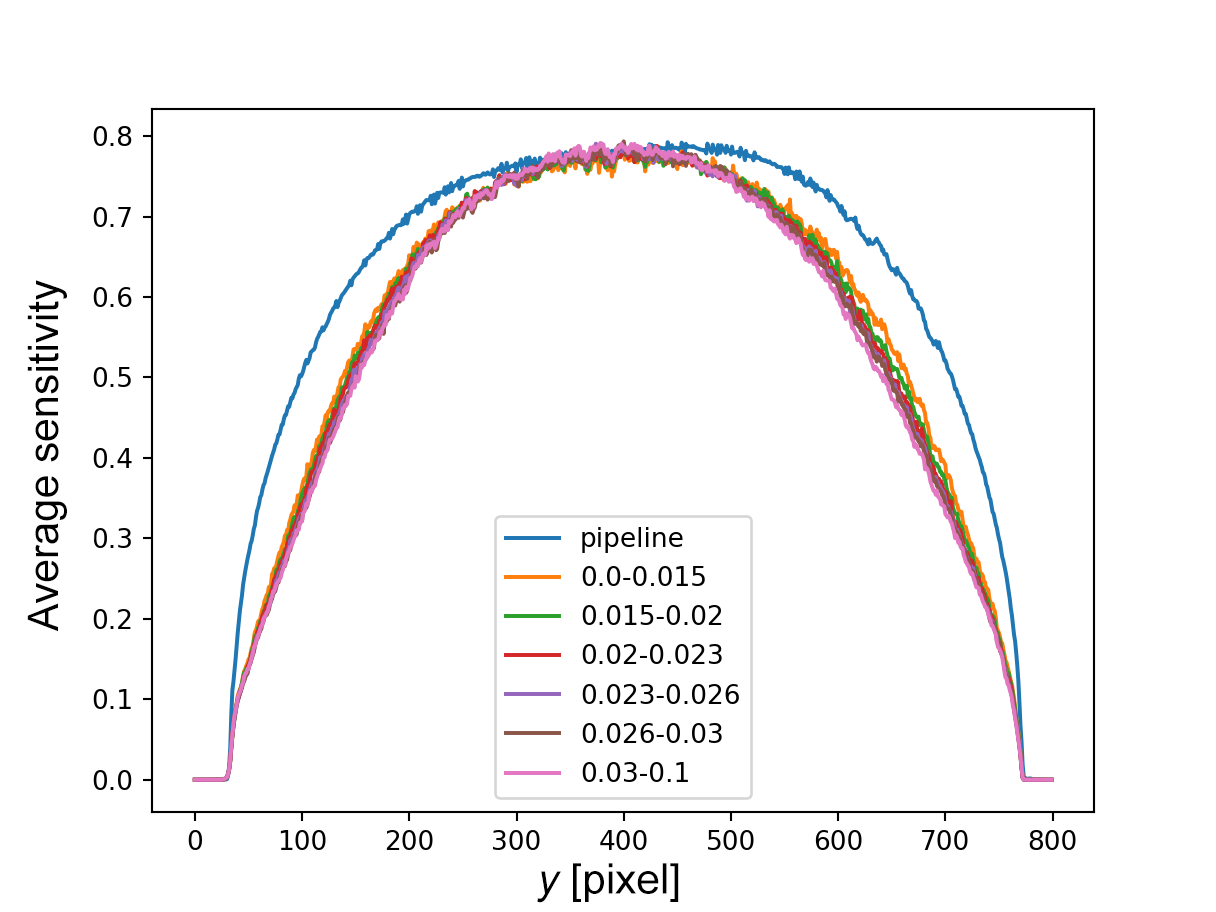
\includegraphics[width=0.48\textwidth]{figures/gs/profile_y-new}
\end{center}
\caption[Profile plots of sensitivity maps]{
  \label{flat-profile}
  \emph{Left:} Profile plots of sensitivity maps in x direction;
  \emph{Right:} Profile plots of sensitivity maps in y direction.
  6 sensitivty maps are constructed by photons from regions with different photon countrate, which are compared with the pipeline sensitivity map.
}
\end{figure}


\section{Galactic plane maps}
\label{maps}
After the aspect solution, distortion map and sensitivity map are calibrated.
The corrected photon data are projected and binned into images as count maps with gnomonic projection.
To scale the effect of relative exposure time, the exposure map is constructed as:
\begin{eqnarray}
Exp(X,Y) &=& \int^{t}f(X(t), Y(t))(1-dead(t))(1-cut(t))dt
\end{eqnarray}
where $f(X(t), Y(t))$ is the sensitivity map measured in Section \ref{sm} and shifted to align with the image.
$dead(t)$ is the electronic dead time of the detector, which is from the spacecraft state file (-scst).
$cut(t)$ is the fraction of the photons that have been cut by $Q$ and $Y_A$ described in Section \ref{data}.
With the count maps and exposure maps, the intensity map is defined as the ratio of them.
Fig.~\ref{flowchart} shows the flowchart of our pipeline.

The full resolution (2 arcsec per pixel) maps are constructed   as $1 \times 2$ deg tiles with 1 deg overlap on each side of the image.
Then the maps are projected into low resolution (nside=2048) \project{Healpix} map.
Fig.~\ref{map0} shows the full Galactic plane divided into 4 equal-sized slices.
In Fig.~\ref{map1}, we also present zoom-in images in four interesting regions where Nebula structures reside.
To qualitatively illustrate the calibration performance in image level, Fig.~\ref{map2} shows the side-by-side comparison between the images generated from the original pipeline calibration and the calibration from this paper.
There are doubling artefact of individual sources and image-level smearing in the original pipeline images (left), which is caused by the imperfect aspect solution.
In comparison, there is no obvious artefact in the images from this paper.

To illustrate the coverage of this data set, Fig.~\ref{map3} shows the all sky Mollweide projection NUV intensity map constructed from from the \asc\ data, the \msc\ data and the \cause\ data (this paper).
The \cause\ data fill most of the sky around the Galactic Plane that have never been observed in the \galex\ main mission.
In Fig.~\ref{map4}, we present the Galactic Plane images from different surveys. 
The structure of Galactic Plane varies dramatically in different wavelength.
\begin{figure}[p]
\begin{center}
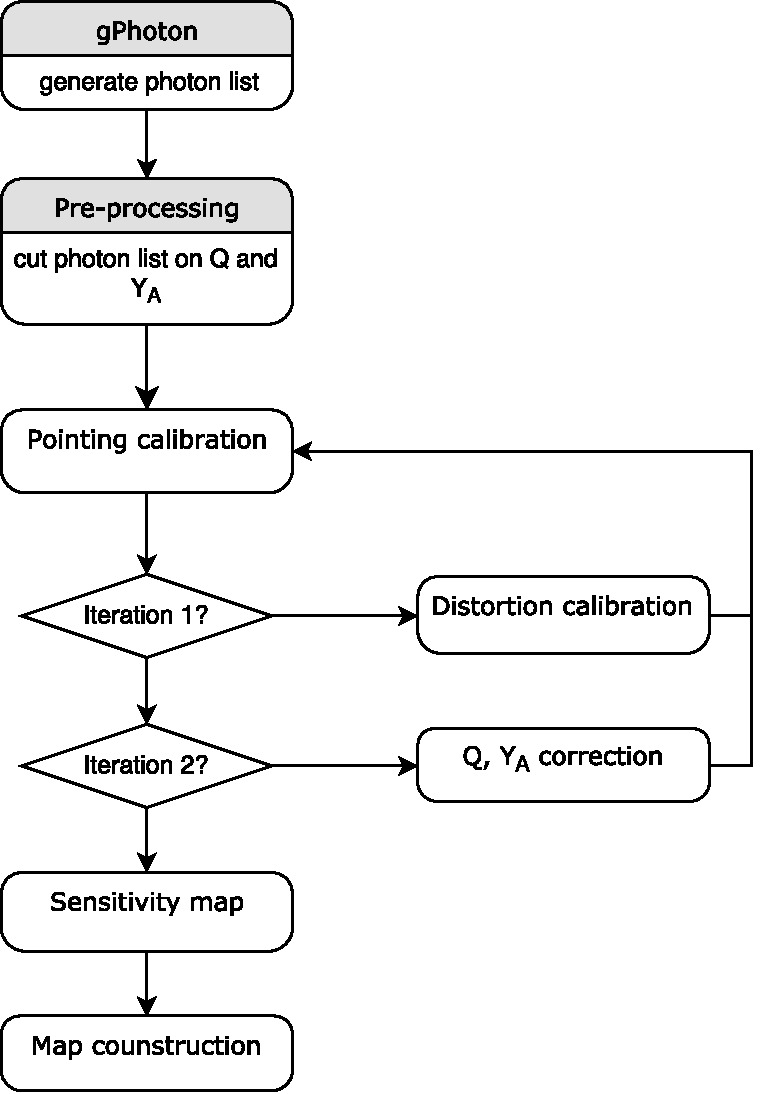
\includegraphics[width=0.6\textwidth]{figures/gs/flowchart}
\end{center}
\caption[The flowchart of the pipeline]{
  \label{flowchart}
  The flowchart of the pipeline.
}
\end{figure}


\begin{figure}[p]
\begin{center}
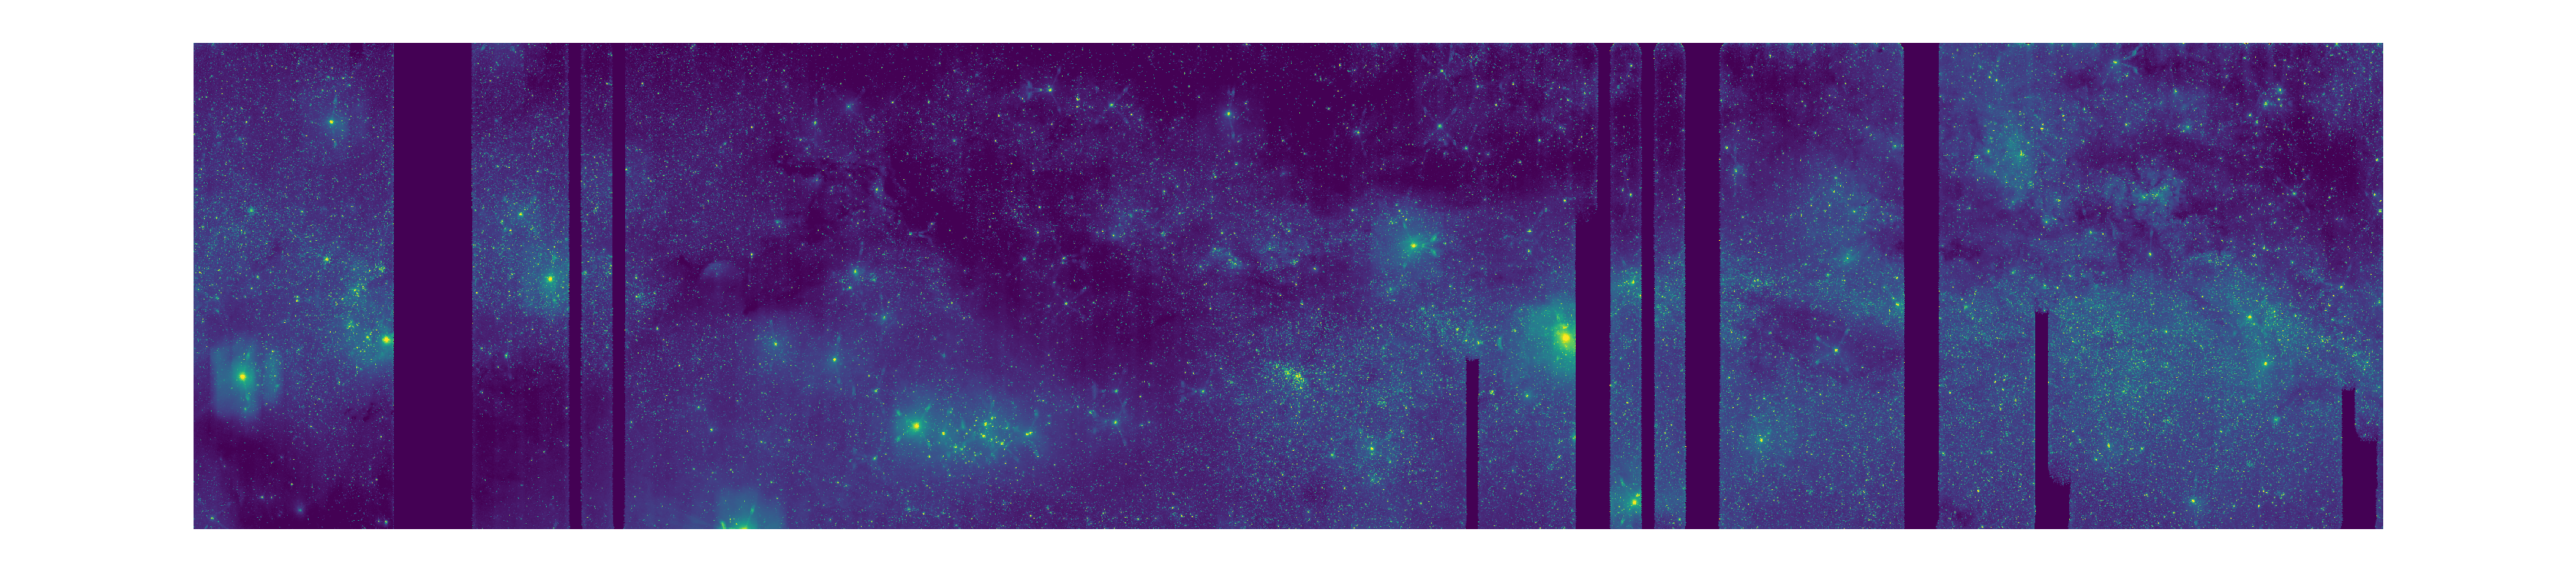
\includegraphics[width=1.\textwidth]{figures/gs/cartview1}
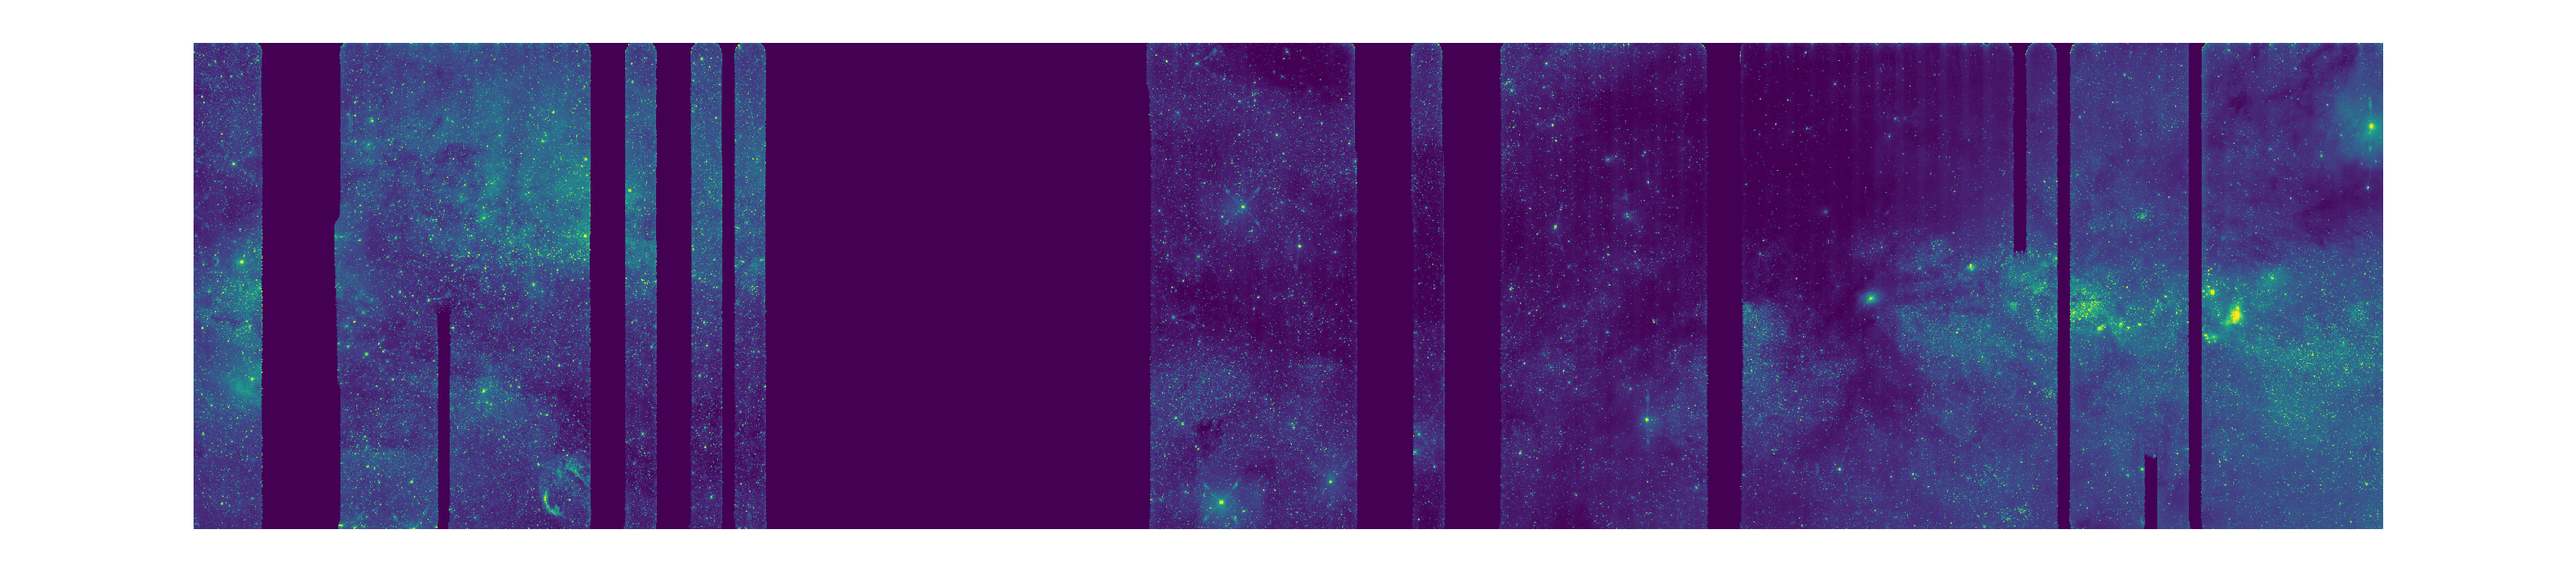
\includegraphics[width=1.\textwidth]{figures/gs/cartview2}
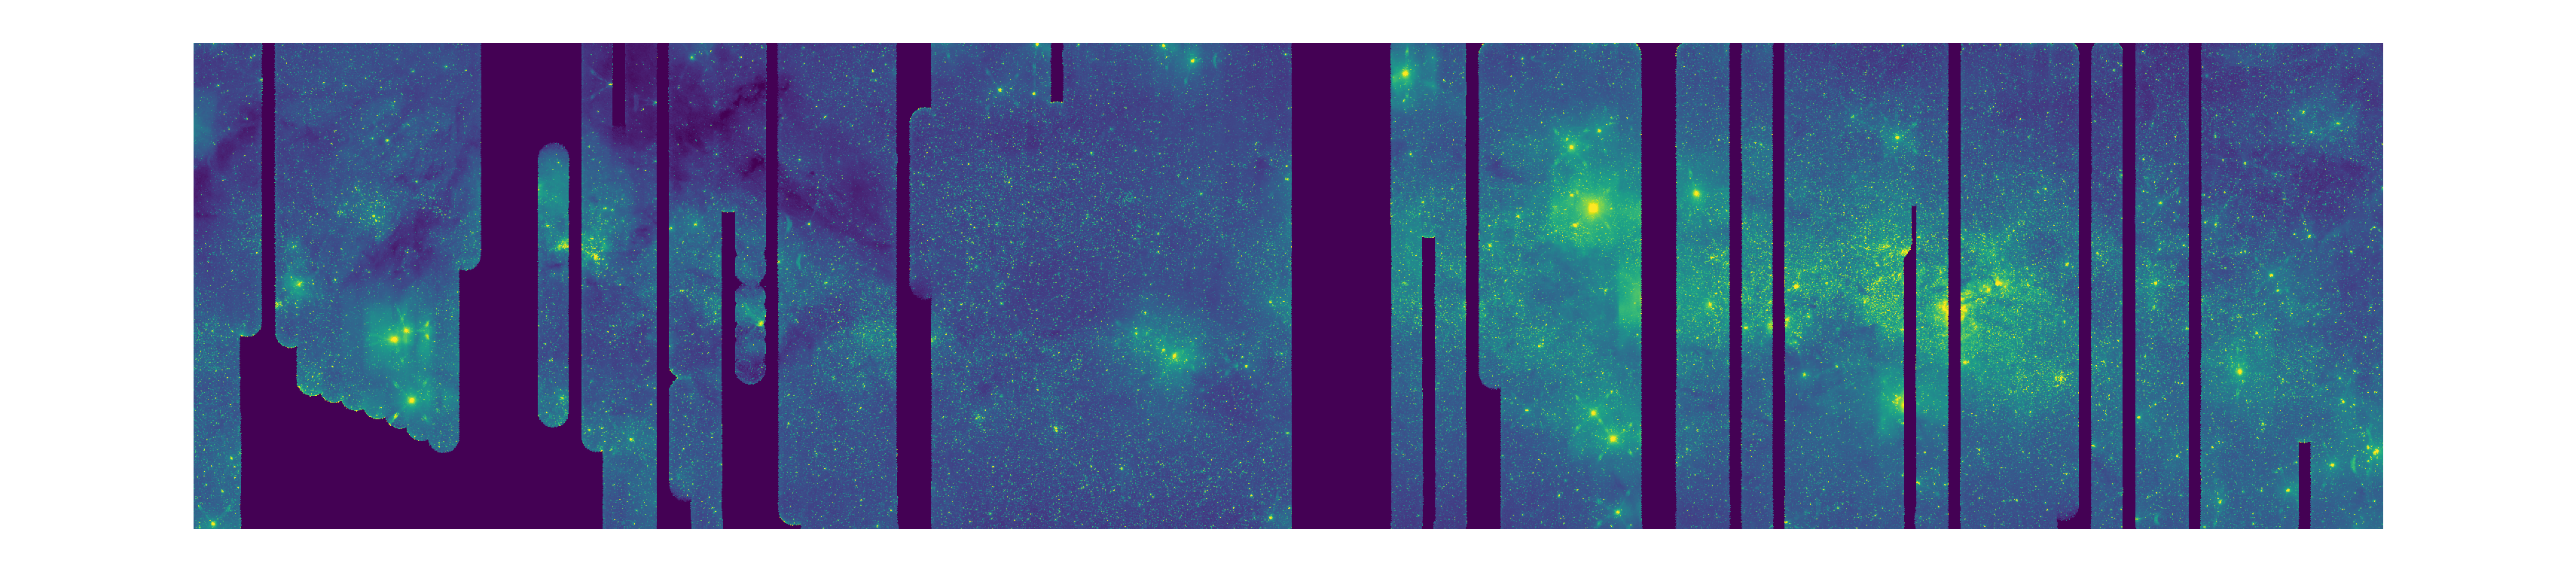
\includegraphics[width=1.\textwidth]{figures/gs/cartview3}
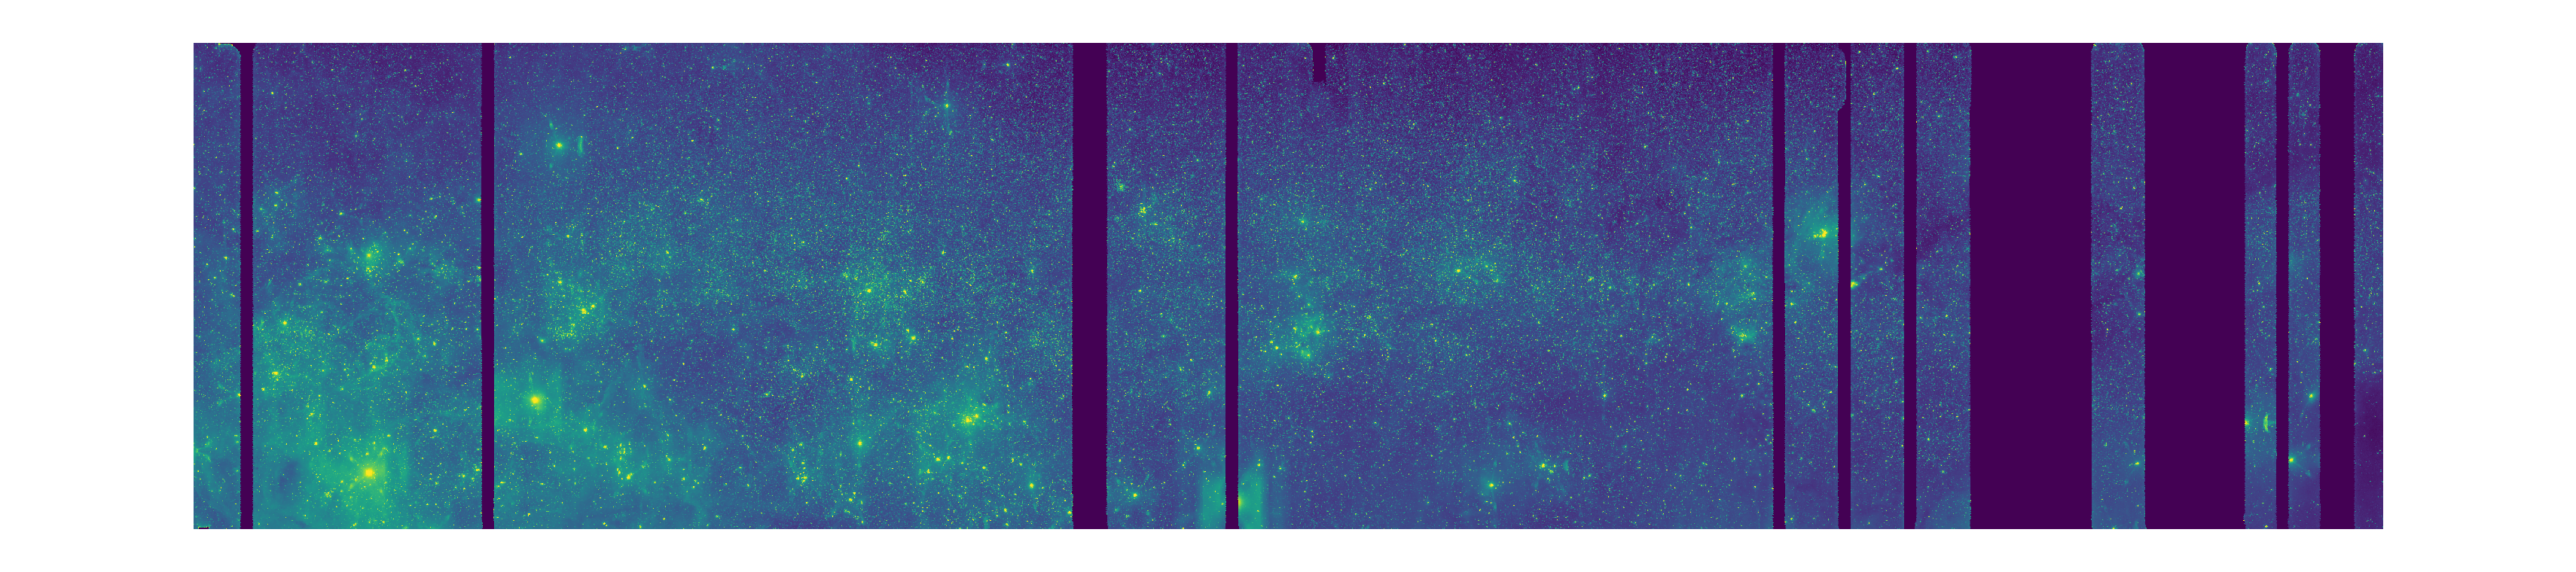
\includegraphics[width=1.\textwidth]{figures/gs/cartview4}
\end{center}
\caption[Calibrated Galactic Plane images]{
  \label{map0}
  Four equal-sized slice of the Galactic Plane($-10<=gb<=10$).
  From top to bottom, the ranges of Galactic longitude are: 90-180 deg, 0-90 deg, 270-360 deg and 180-270 deg.
}
\end{figure}

\begin{figure}[p]
\begin{center}
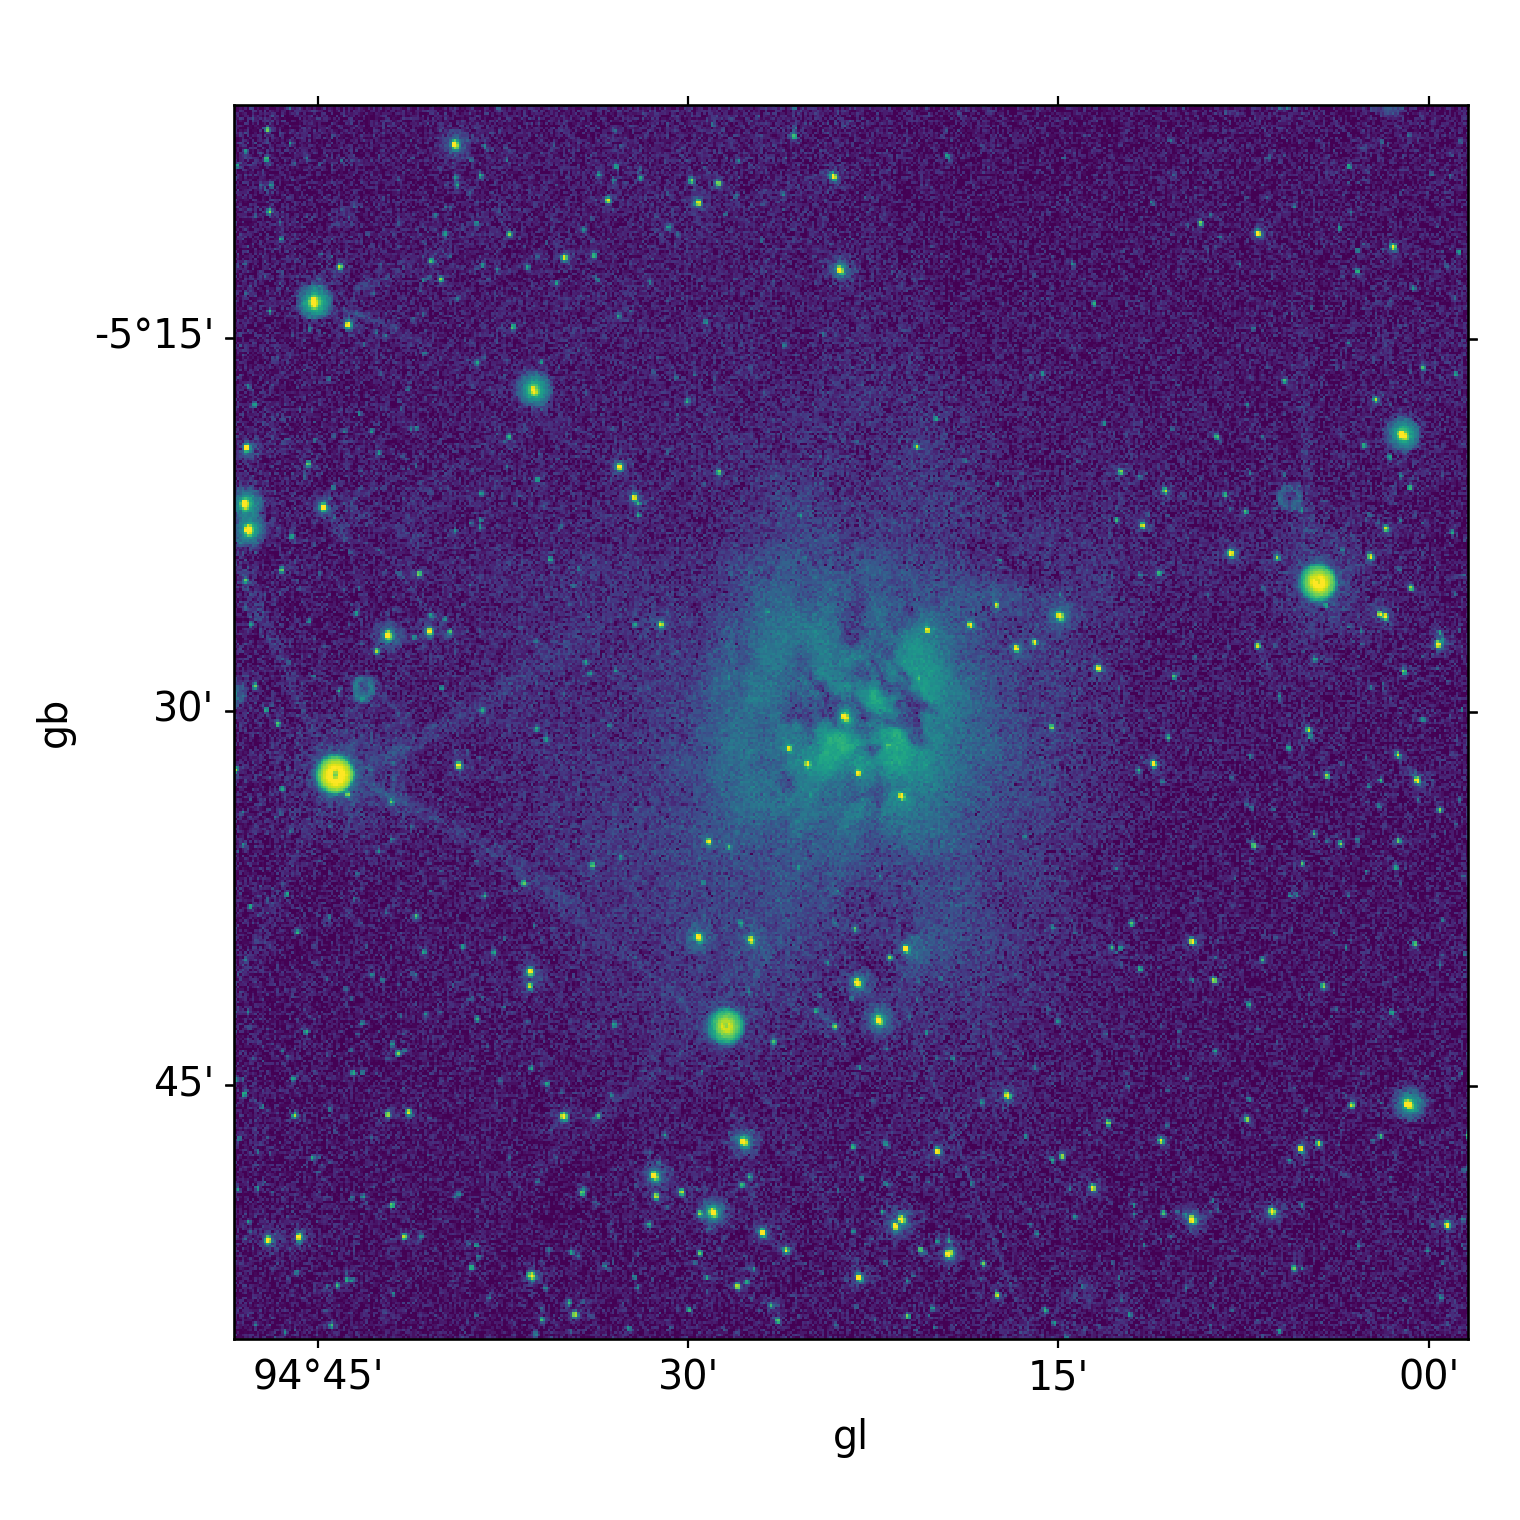
\includegraphics[width=0.49\textwidth]{figures/gs/cocoon}
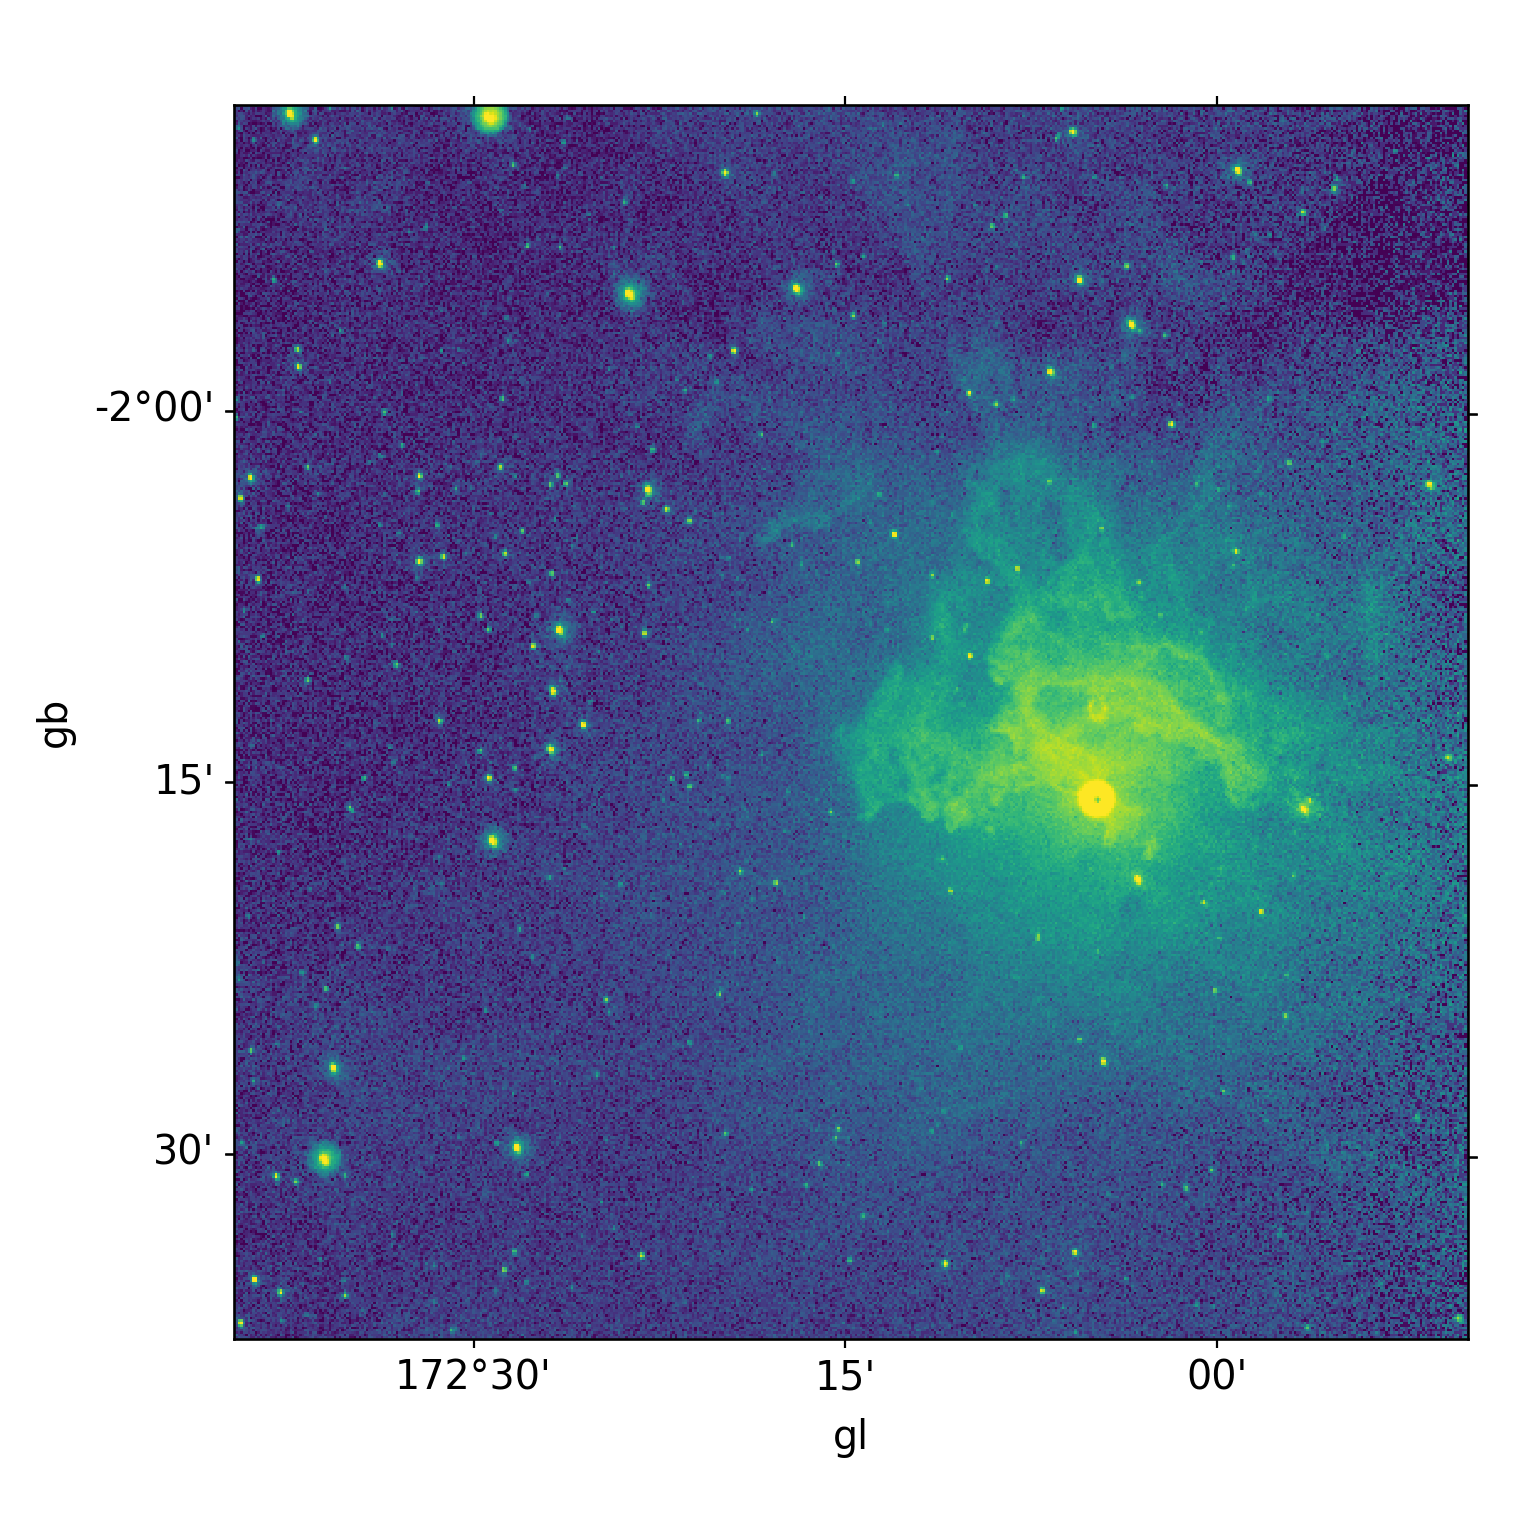
\includegraphics[width=0.49\textwidth]{figures/gs/FlamingStar}
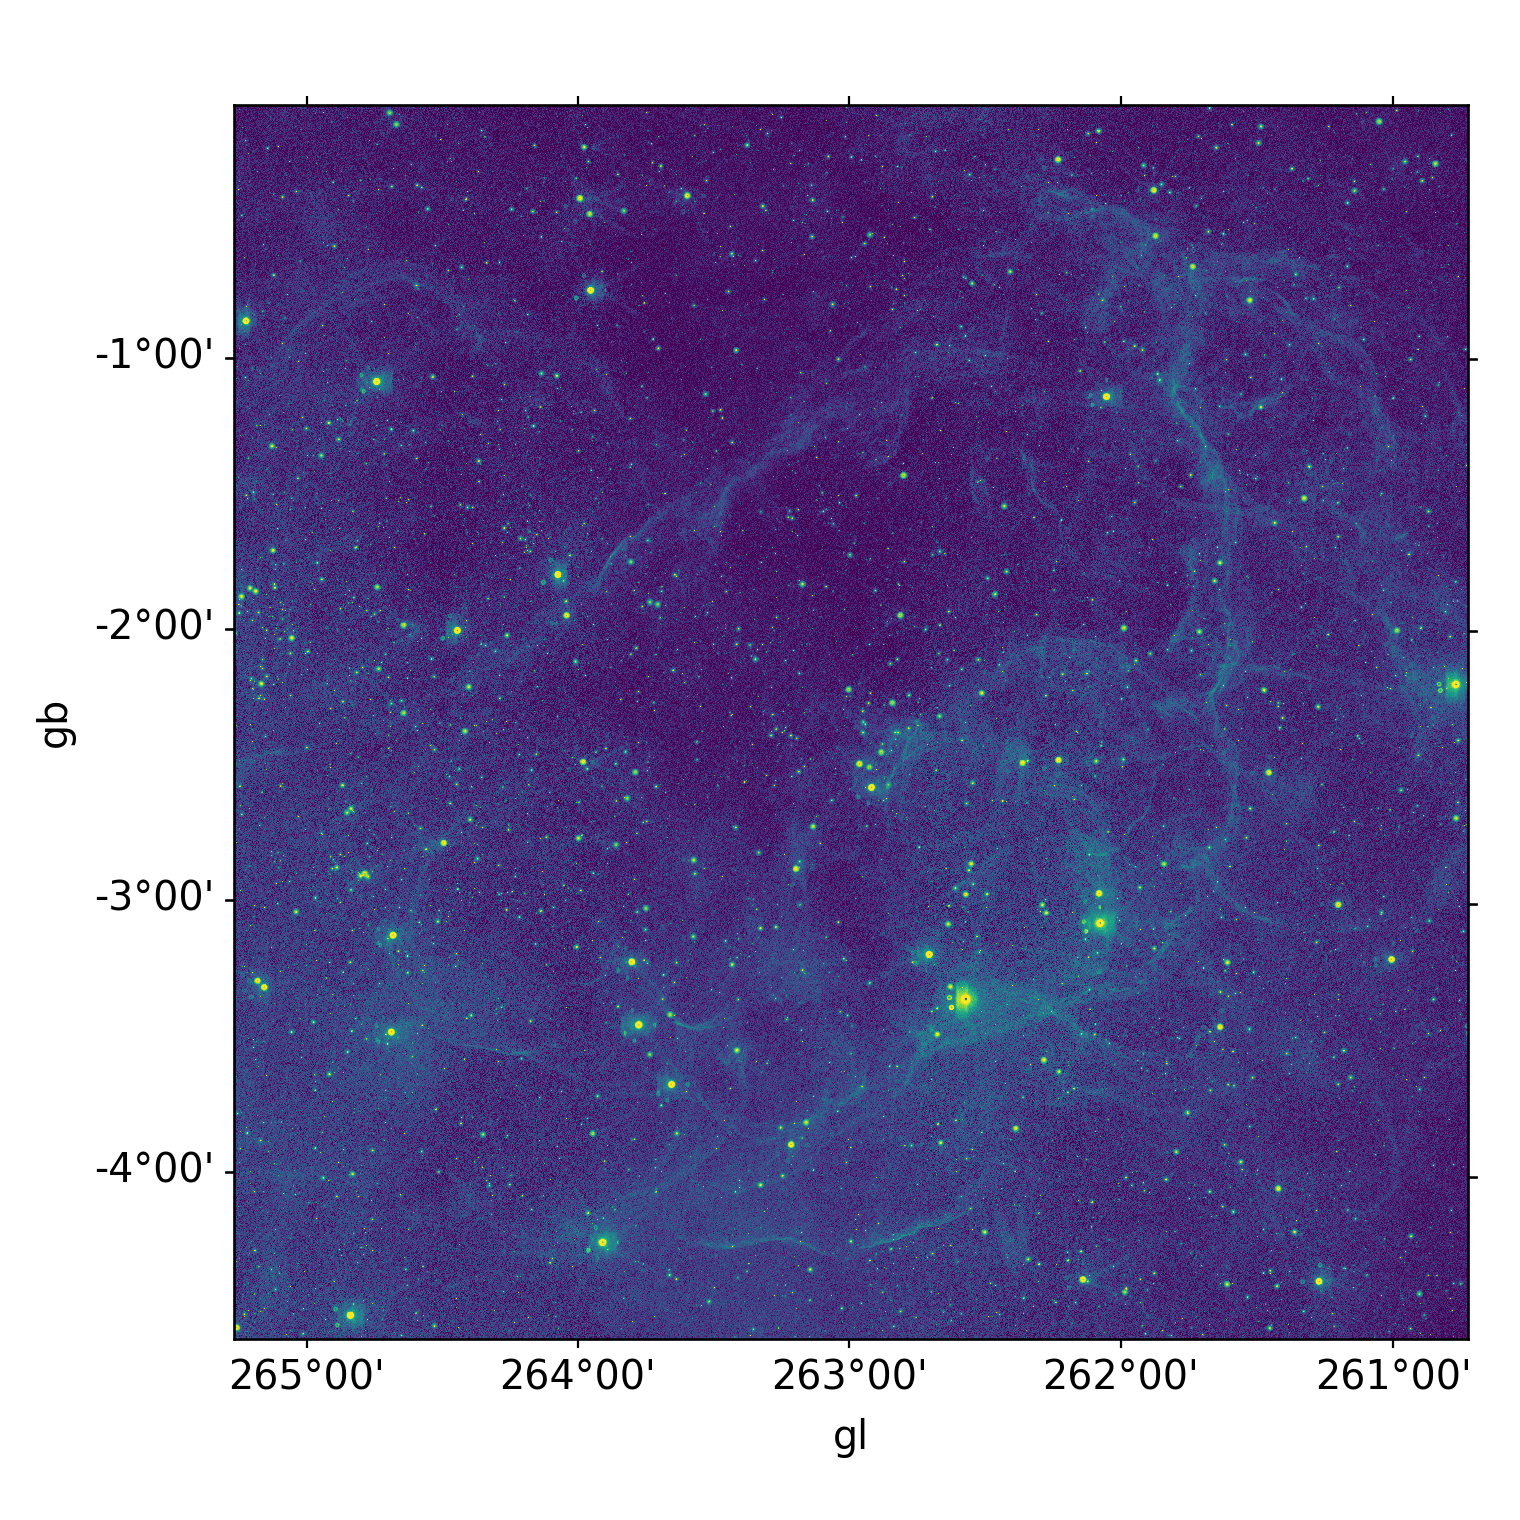
\includegraphics[width=0.49\textwidth]{figures/gs/vela}
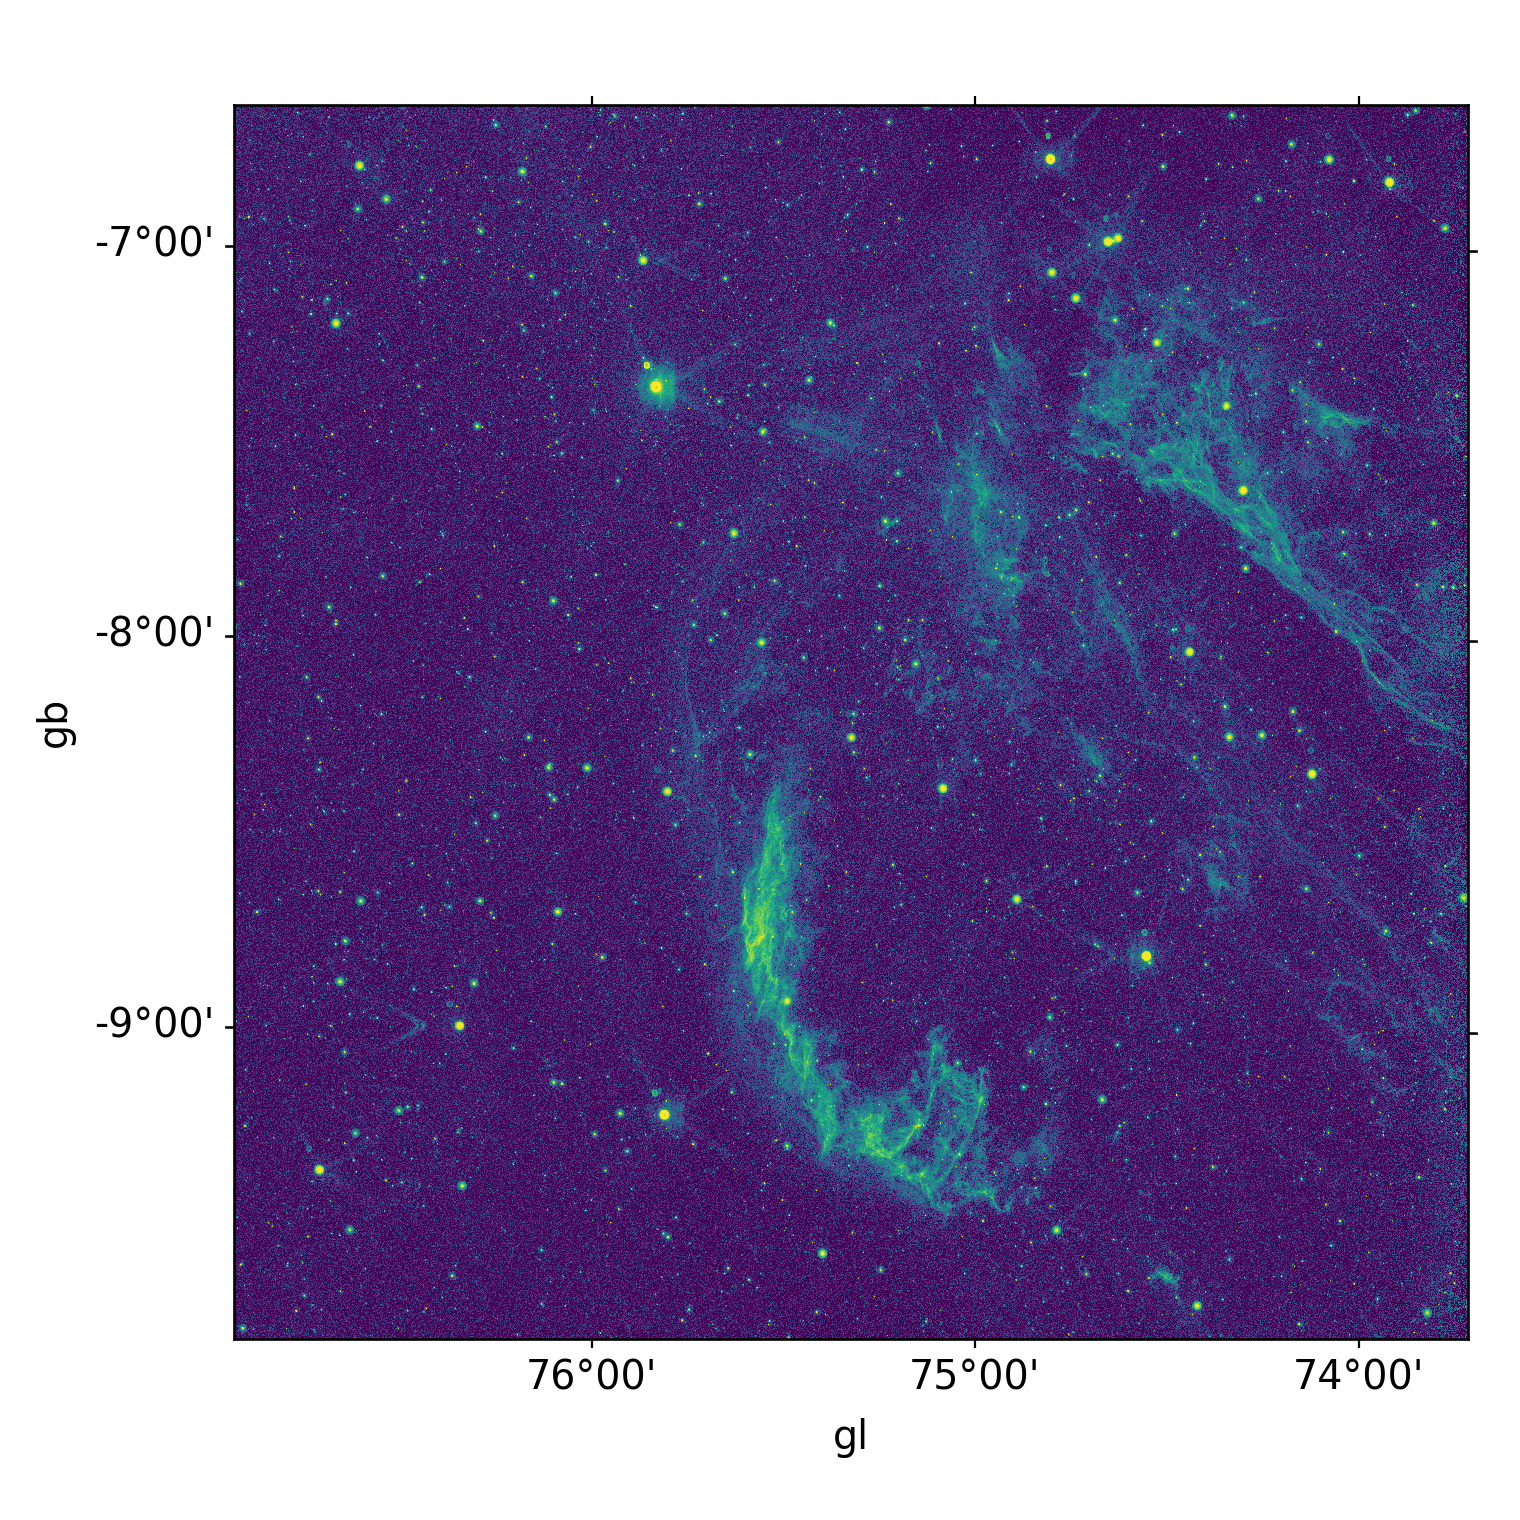
\includegraphics[width=0.49\textwidth]{figures/gs/cygnusloop}
\end{center}
\caption[Calibrated Galactic Plane images: zoom-ins]{
  \label{map1}
   \emph{Top-left:}  the Cocoon Nebula;
   \emph{Top-right:} the Flaming Star Nebula;
   \emph{Bottom-left:} the Vela Supernova Remnant;
   \emph{Bottom-right:} the Cygnus Loop Nebula.
}
\end{figure}

\begin{figure}[p]
\begin{center}
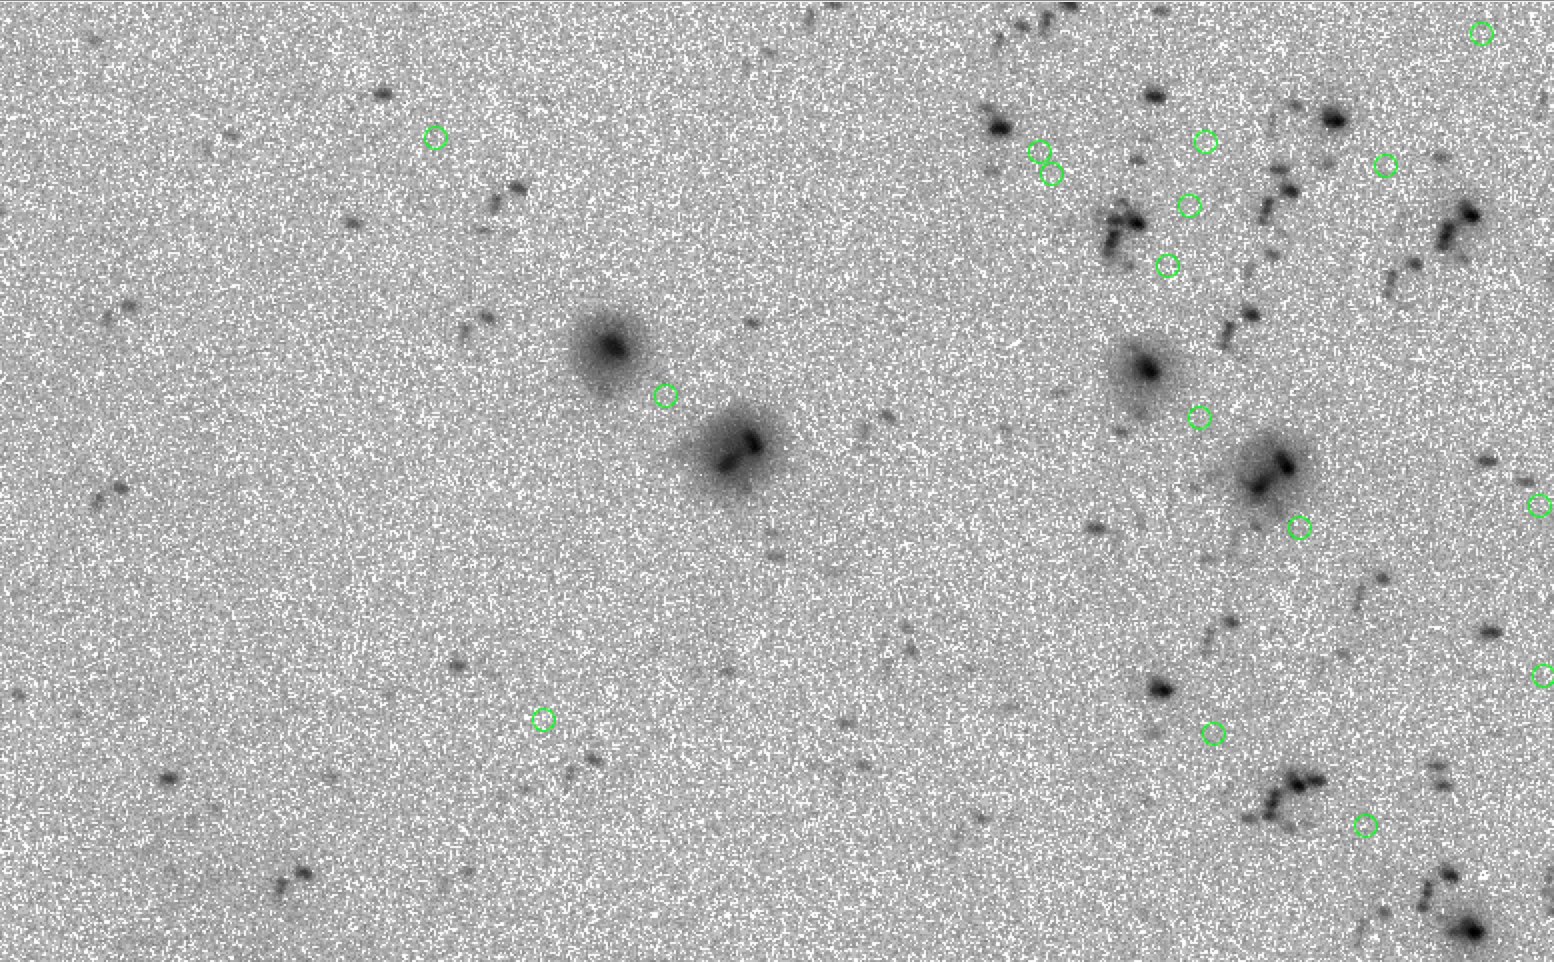
\includegraphics[width=0.49\textwidth]{figures/gs/pip0}
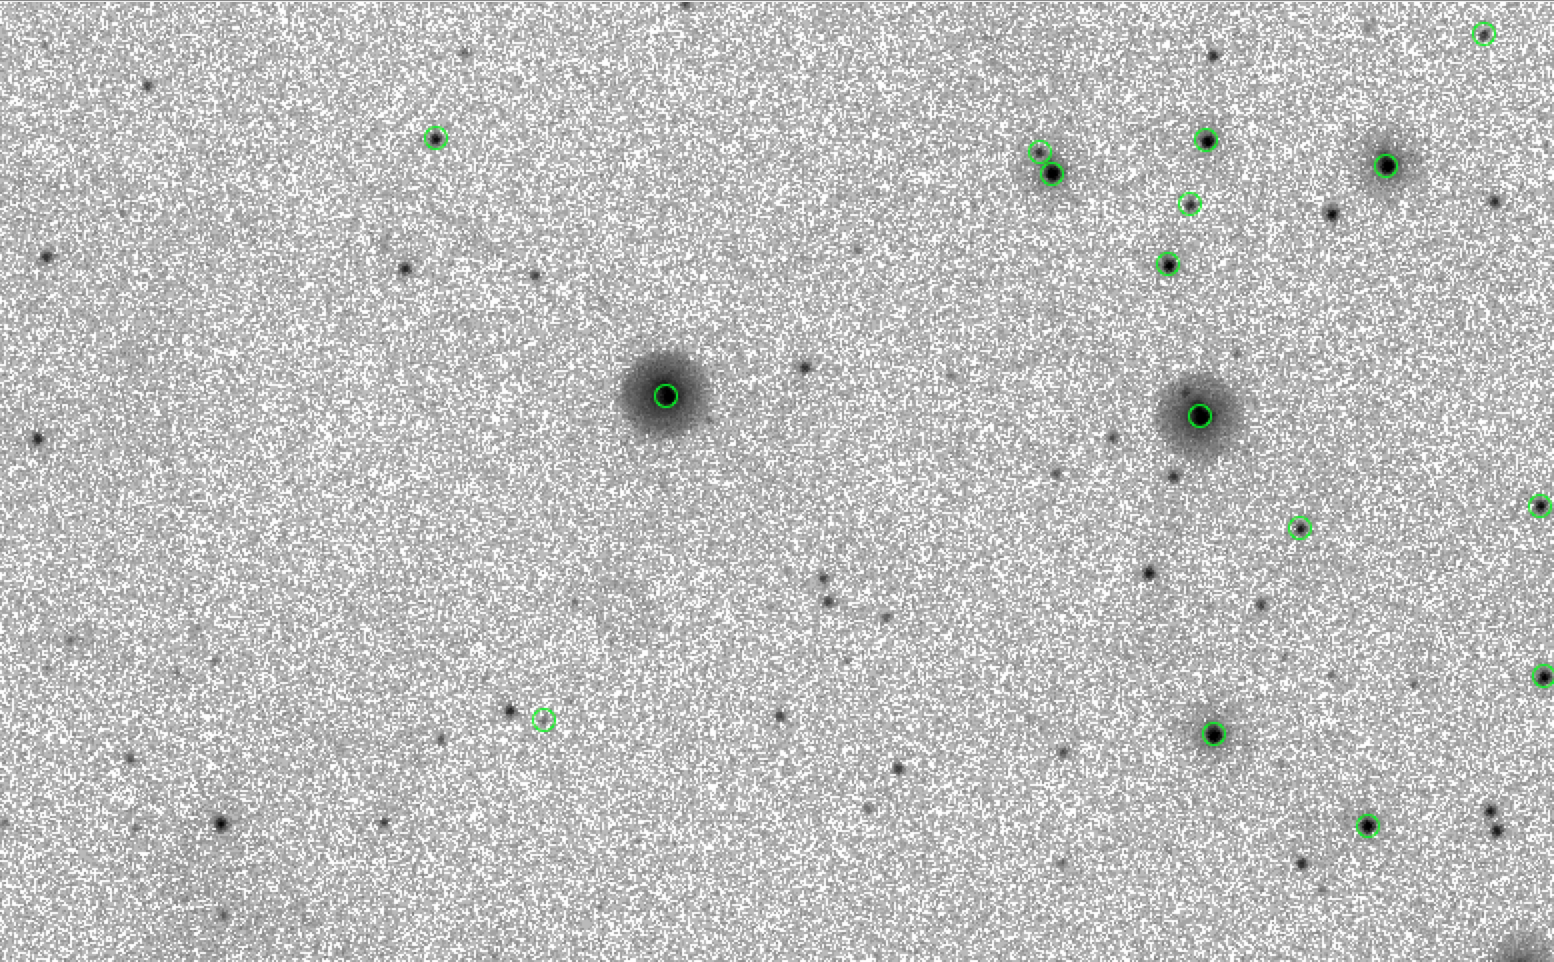
\includegraphics[width=0.49\textwidth]{figures/gs/cal0}
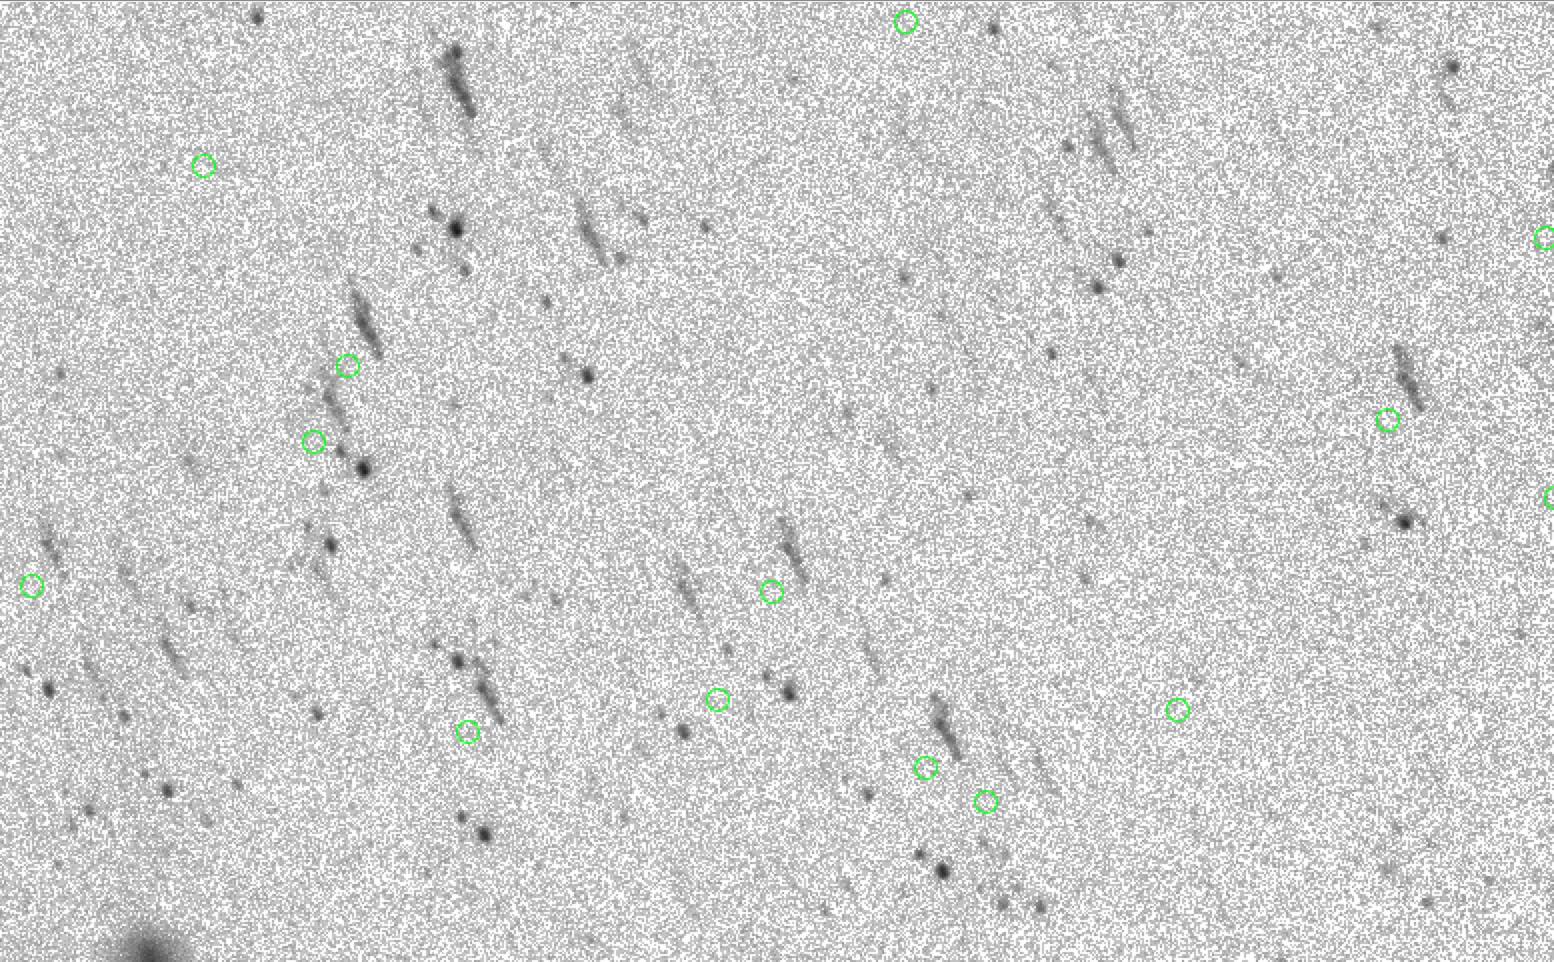
\includegraphics[width=0.49\textwidth]{figures/gs/pip1}
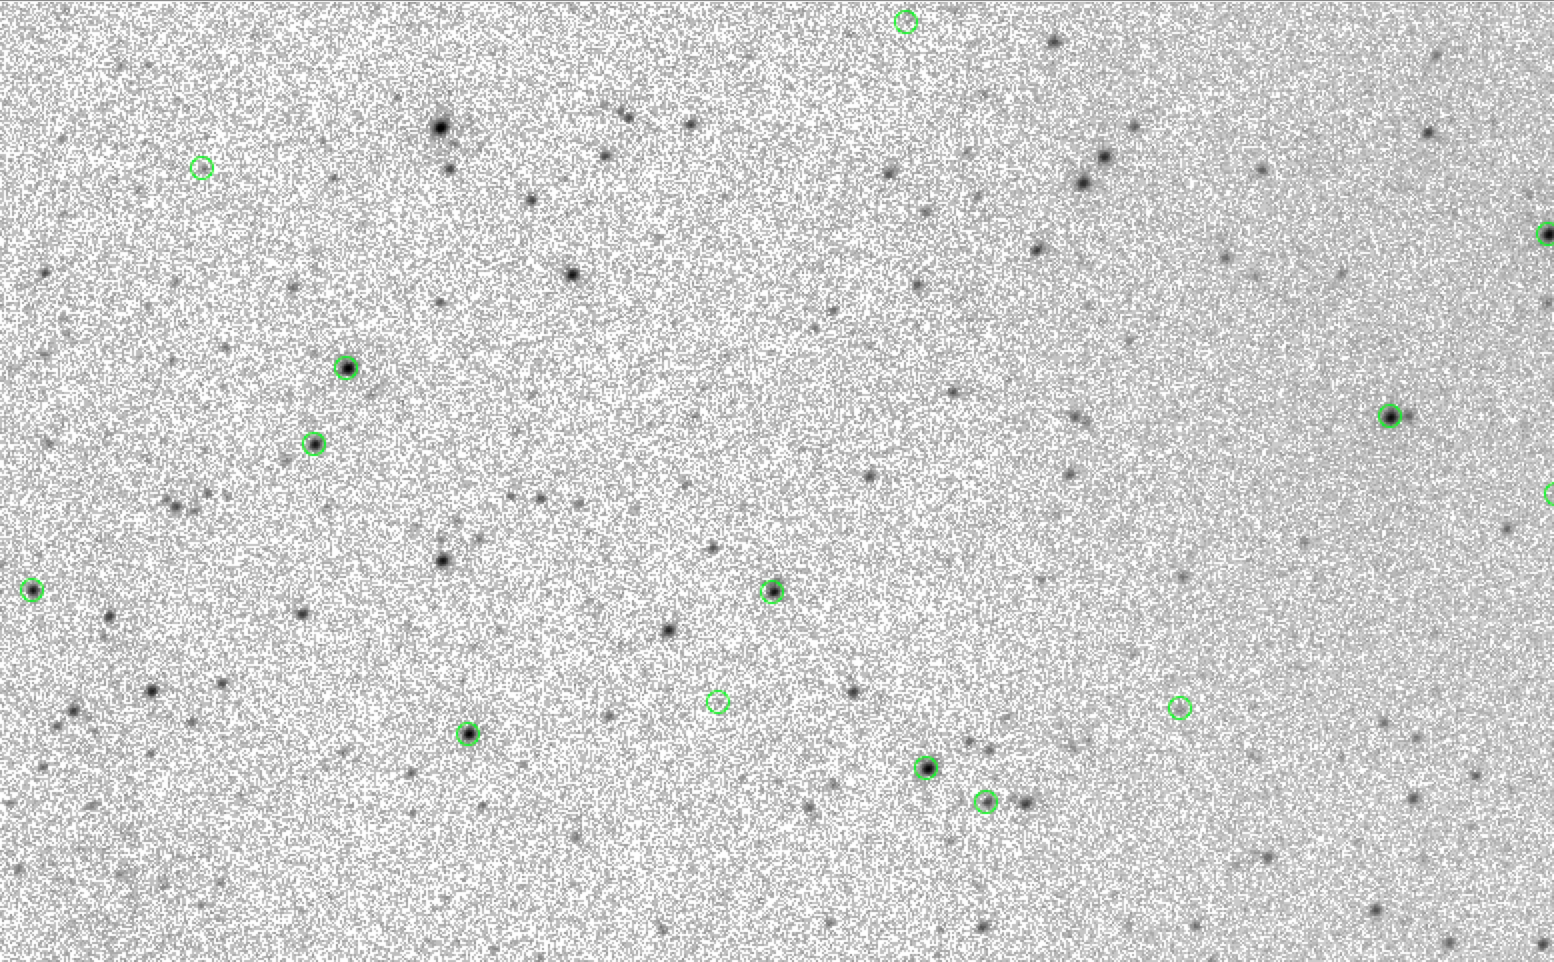
\includegraphics[width=0.49\textwidth]{figures/gs/cal1}
\end{center}
\caption[Comparison with the images generated by the original calibration pipeline]{
  \label{map2}
  Side-by-side comparison with the images generated by the original calibration from the telescope.
  \emph{Left:} images from the orignal pipeline;
  \emph{Right}: images from our pipeline.
  The stars from Tycho 2 catalog are marked by the green circle.
}
\end{figure}

\begin{figure}[p]
\begin{center}
\includegraphics[width=1.\textwidth]{figures/gs/overlap}
\end{center}
\caption[The coverage of \asc, \msc and \scanmode\ data]{
  \label{map3}
  All sky Mollweide projection in Galactic coordinates of the NUV intensity maps.
  The \asc\ data are plot in grey scale.
  The \msc\ data are plot in RdBu scale.
  The \scanmode\ data are in Viridis scale. 
}
\end{figure}

\begin{figure}[p]
\begin{center}
\includegraphics[width=0.99\textwidth]{figures/gs/multi1}
\end{center}
\caption[The Galactic Plane in multi-wavelength]{
  \label{map4}
  The Galactic Plane in multi-wavelength. From top to bottom, the data are from:
  \project{Planck} 100 $GHz$; \project{Wise} 3.4 $\mu m$; H-alpha; \cause.
}
\end{figure}

\section{Discussion}
\label{ds}

In this paper, we have presented a calibration pipeline for the \cause\ data, which performed both high precision astrometric and photometric calibration for this dataset for the first time.
The spacecraft attitude solution is measured by cross-correlating the photons and stars.
The point of the cross-correlation is that we can figure out the spacecraft pointing using stars, but without ever actually running any kind of star detector in the raw data.
The only assumption underlying is that most of the object in the field are nearly point sources.
This avoided any choices about how stars are detected.
It is important especially when the field is crowded (which is true in the Galactic Plane), since source detection and centroid measurement is hard in such field.
However the disadvantage is that by directly using the star catalog, the astrometric calibration precision is limited by the precision of the catalog itself.
One possible improvement is to decouple the relative astrometric calibration from the absolute calibration.
That is to cross-correlate photons within different time slots to first measure the relative attitude solution and then use the star catalog to calibrate the overall absolute pointing in the sky.
By doing this it might be possible to achieve higher precision and maintain the same overall accuracy for the astrometry.

To calibrate the sensitivity map, a self-calibration approach similar to \cite{uber} is adopted, in which the relative sensitivity is measured by assuming that stars are constant over time and the repeated observations of the same stars are utilized. 
The speciality in this paper is that the sensitivity map in different count rate condition is constructed independently to account for the large dynamic range of count rate in this dataset.
However as all relative calibration approach, the absolute scale of the sensitivity map can not be determined without any external information.
For the \cause\ data, the overall photometric zero point can be determined by matching the stars with the original \galex\ catalog and let them agree with each other.
This will be discussed in detail in the catalog paper (Mohammed et al., in prep).

In this paper the photons with $Q<=5$ or $Y_A<2$ are removed to avoid contamination from these highly biased photons as described in \ref{data}.
There are around 70 percent photons remained after the cut.
However, as shown in Fig.~\ref{meta}, the overall offsets of photons with $Q<5$ is not totally randomly distributed.
Therefore, instead of removing these photons, it is possible to measure the average offset of photons as a function of $Q$ and correct the offset.
If this correction could be achieved, there will be additional 30 percent photons available, which could increase the signal to noise of the imaging data by significant amount.

In conclusion, despite all these potential improvements mentioned above, the high precision calibration of NUV imaging data for the Galactic Plane is available for the first time using \galex. 
Research like \cite{redclump} has already shown that the UV-optical color is an unique probe of physical properties for red clump stars.
We expect that by calibrating and making the \cause\ data available, it could make plenty of research opportunities possible in Galactic astronomy.

\section{Chapter acknowledgements}
\galex (Galaxy Evolution Explorer) is a NASA Small Explorer, launched in 2003 April.
This work is based on data from the Tycho 2 catalog (\url{https://www.cosmos.esa.int/web/hipparcos/tycho-2}).
This research made use of Astropy, a community-developed core Python package for Astronomy \citep{astropy}.
The data analysis presented in this article was partially performed on computational resources at NYU HPC.

